
\input{"header.tex"}



%Here is some text, where we use APC.\nomenclature{APC}{antigeen-presenterende cel}

%\printnomenclature

% -----------------------------------------------------------------------------
% Introduction and research problem

\chapter{Introduction to Neutrino Physics}
\label{c:theoryIntro}

\section{Research Goals}
The research in this thesis describes the construction of a prototype Magnetized Iron Neutrino Detector (Baby MIND) at the European Organization for Nuclear Research (CERN) and determine the performance of the detector to reconstruct charged particle tracks at a test beam at CERN and neutrino interactions with our collaborators in the WAGASCI collaboration at a neutrino beam at the JPARC facility in Japan. This is discussed further in chapter~\ref{c:WAGASCI}.

%This research aims to construct a prototype Magnetized Iron Neutrino Detector (Baby MIND) at the European Organization for Nuclear Research (CERN) and understand the performance of the detector to reconstruct charged particle tracks at a test beam at CERN and neutrino interactions with our collaborators in the WAGASCI collaboration at a neutrino beam at the JPARC facility in Japan. This is discussed further in chapter~\ref{c:WAGASCI}.

\section{Neutrino discovery}\label{section:Theory}
While measuring radioactive beta decay, from bombarding beryllium with alpha particles from polonium, in the first two decades of the 20th century, physicists discovered what was then an anomaly. At the time it was thought that beta decay occurred as a two body process in which a neutron ($n$) decays to a proton ($p$) and electron ($e^-$). If this were the case, the energy of the proton and electron should be discrete and add up to the energy of the neutron. However experiments showed that the electron had a continuous spectrum of energy values, violating the energy conservation law, as seen in \FigRef{fig:betaeng}. In order to solve this anomaly, a third particle, the neutrino ($\nu$), was postulated by Wolfgang Pauli \cite{4Pauli:Online} and then incorporated into the beta decay by Enrico Fermi \cite{5Wilson}. The neutrino was postulated as a neutral particle with mass of less than 1\% of the proton mass and a spin of 1/2. For consistency, the particle produced in the beta decay is relabelled as the electron antineutrino, $\bar{\nu_e}$, in order to conserve lepton number. The addition of another particle changed the decay to $n \rightarrow p + e^- + \bar{\nu_e}$ and introduced the weak interaction model, as seen in \FigRef{fig:beta}. 

\begin{figure}[h!]
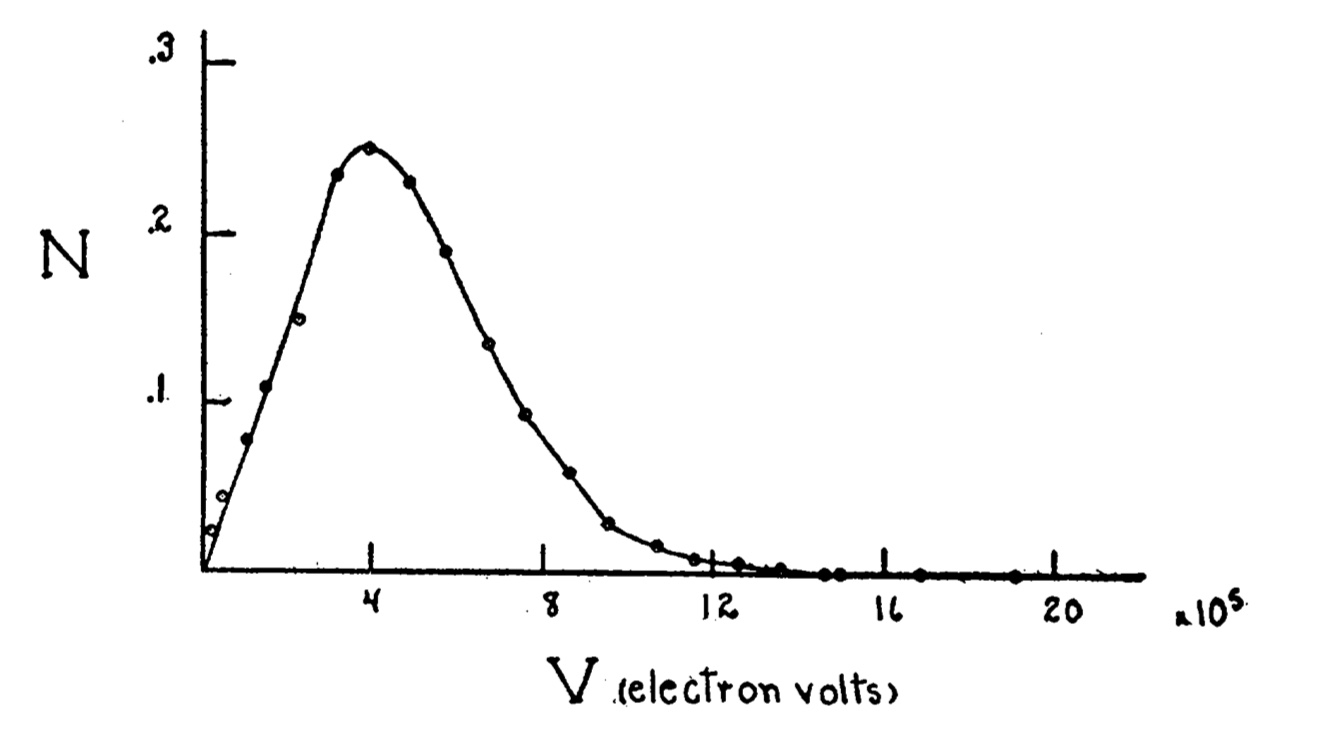
\includegraphics[width=\textwidth]{figures/betaRadium.jpeg}
\caption{The kinetic energy spectrum of the emitted electron from beta decay from a Radium-E source~\cite{RadiumE}. If no anti-neutrino were emitted a single electron volt(s) value would be expected.}
\label{fig:betaeng}
\end{figure}

\begin{figure}[h!]
\centering
\begin{subfigure}{.5\textwidth}
  \centering
  \begin{fmffile}{badBeta}
\begin{fmfgraph*}(120,80)
\fmfstraight
\fmfleft{i1,i2,o1}
\fmfright{o2}

\fmf{fermion}{i1,v1}
\fmf{fermion}{v1,o1}

%fmf{boson}{v1,v2}
\fmf{fermion}{v1,o2}

\fmflabel{n}{i1}
\fmflabel{p}{o1}
\fmflabel{$e^{-}$}{o2}
\end{fmfgraph*}
\end{fmffile}
\vspace{2mm}
  \caption{The initially assumed beta decay}
  %\label{fig:sub1}
\end{subfigure}%
\begin{subfigure}{.5\textwidth}
  \centering
  \begin{fmffile}{beta}
\begin{fmfgraph*}(120,80)
\fmfstraight
\fmfleft{i1,i2,o1}
\fmfright{o2,o3}

\fmf{fermion}{i1,v1}
\fmf{fermion}{v1,o1}

\fmf{boson}{v1,v2}
\fmf{fermion}{v2,o2}
\fmf{fermion}{o3,v2}

\fmflabel{n}{i1}
\fmflabel{p}{o1}
\fmflabel{$e^{-}$}{o2}
\fmflabel{$\bar{\nu}_e$}{o3}
\end{fmfgraph*}
\end{fmffile}
\vspace{2mm}
  \caption{Correct beta decay}
  %\label{fig:sub2}
\end{subfigure}
\vspace{2mm}
\caption{Feynman diagrams showing beta decay.}
\label{fig:beta}
\end{figure}

It would take another twenty years until the neutrino was experimentally discovered by the Savannah river reactor experiment in 1956~\cite{6Reines} where neutrinos from a nuclear reactor were detected in 300 litres of liquid scintillator and cadmium. The experiment was awarded the Nobel prize in 1995.

After the discovery of the electron neutrino ($\nu_e$), several neutrino experiments were performed and led to the discovery of two other neutrino types/flavours, the muon neutrino ($\nu_\mu$) and the tau neutrino ($\nu_\tau$)~\cite{7Danby, 8Perl, Fix1}.

\if{0}
\textbf{Put in V-A theory here? weak interaction model. Fermi theory?}
\textbf{Expand with parity violation etc etc?}

Explain QED, use this plus experiments (chirality etc) to introduce a modified QED for weak interactions, V-A theory. Using this find neutral current experiment which is not in V-A theory leading to electroweak unification.
Start with dirac lagrangian, impose local gauge invariance produces a massless vector field A, set A as the photon field and we are done! 
Very few details, more in Peskin and Schroeder and other books.
\textbf{Mix in experiments!}
\fi

To describe the neutrino interactions it is worth building a theory to try to describe the interactions. 

Starting with the generalized and relativistic version of the Schro\"{o}dinger equation, the Dirac equation:
\begin{equation}
\sum_\mu (i\gamma^\mu \partial_\mu - m)\psi(x) = 0
\end{equation}
where $\gamma$ are the so called Dirac matrices and the sum over $\mu$ is often removed using the Einstein notation requiring any free index to be summed over.

As with all quantum mechanical equations this allows us to define $\psi(x)$ as a quantum field/state.

After taking Lorentz-invariance into account the Dirac Lagrangian can be written as:
\begin{equation}
\mathcal{L} = \bar{\psi}(i\gamma^\mu\partial_\mu-m)\psi
\end{equation}
where the Euler-Lagrange equation for $\bar{\psi}$ reproduces the Dirac equation.

The Lagrangian is so far correct, however from a physical point of view the equation also needs to be invariant under a phase shift, so called gauge transformation $\psi \rightarrow e^{i\theta(x)}\psi$. This requires the addition of an extra term to remove the terms which prevent gauge invariance providing the full Dirac Lagrangian as:

\begin{equation}
\mathcal{L} = \bar{\psi}(i\gamma^\mu\partial_\mu-m)\psi -q\bar{\psi}\gamma^\mu\psi\epsilon_\mu \equiv \mathcal{L}_{Dirac}
\end{equation}
with $\epsilon_\mu$ being a new field which must gauge invariant and q conserved quantity, a numerical constant.

There is now a mathematical framework to describe quantum states or particles in a vacuum. It is now possible to create a framework for a particle interacting with a electromagnetic field by combining $\mathcal{L}_{Dirac}$ with the classical $\mathcal{L}_{Maxwell} = \frac{-1}{4}F_{\mu\nu}F^{\mu\nu} $ with $F^{\mu\nu} = \partial^\mu A^\nu - \partial^\nu A^\mu$ where $A_\mu$ is the electromagnetic vector potential, a 4-vector combined of the electric potential and magnetic potential. 

This produces the following Lagrangian:
\begin{equation}
\mathcal{L} = \mathcal{L}_{Dirac} + \mathcal{L}_{Maxwell} = \bar{\psi}(i\gamma^\mu\partial_\mu-m)\psi -q\bar{\psi}\gamma^\mu\psi\epsilon_\mu - \frac{1}{4}F_{\mu\nu}F^{\mu\nu}
\end{equation}

There is nothing preventing us from choosing our previous field $\epsilon$ as the electromagnetic vector potential $A$ and choosing $q$ as the electron charge $e$ to produce the experimentally verified Lagrangian for quantum and electromagnetic interactions or Quantum ElectroDynamics (QED):

\begin{equation}
\mathcal{L}_{QED} \equiv \bar{\psi}(i\gamma^\mu\partial_\mu-m)\psi -e\bar{\psi}\gamma^\mu\psi A\mu - \frac{1}{4}F_{\mu\nu}F^{\mu\nu}
\end{equation}
This can be simplified by introducing the gauge covariant derivative $D_\mu \equiv \partial_\mu + ieA_\mu$ and the slash notation as $\displaystyle{\not} D = \gamma^\mu D_\mu$. This produces the simplified QED Lagrangian as:
\begin{equation}
\mathcal{L}_{QED} = \bar{\psi}(i\gamma^\mu \displaystyle{\not} D_\mu-m)\psi - \frac{1}{4}F_{\mu\nu}F^{\mu\nu}
\end{equation}

%\textbf{Add example of interaction?} 
%\textbf{electron muon scattering? and introducing Feynman diagrams}

Based on the experiments relating to $\beta$-decay, Fermi hypothesised that the Lagrangian for weak interactions should be similar to the QED Lagrangian. To handle the observed differences, a constant is added $G_F$ to replace the electron charge, and mass removed. QED contains $\gamma^\mu$ meaning that it transforms as a vector which was confirmed by experiments. For weak interactions anything could be mathematically possibly. The absence of Fierz interference terms, parity violation and the Goldhaber helicity experiment made it clear that the interactions had to transform as vectors and axial vectors giving the term $\gamma^\mu - \gamma^\mu \gamma^5 =  \gamma^\mu (1- \gamma^5)$ and also providing the theory with its name: V-A theory. 

This produced a Lagrangian in the form of 
\begin{equation}
\mathcal{L} = \frac{G_F}{\sqrt{2}}J_L \cdot J_H
\end{equation}
with $J_L$ as the current describing interactions with leptons and $J_H$ describing interactions with hadrons (up and down quarks instead of protons and neutrinos). The Fermi constant $G_F$ was also added to substitute the electron charge. The currents were initially of the form:
\begin{equation}
J_L = \bar{\psi}_e(x)\gamma^\mu (1-\gamma_5) \psi_\nu(x)
\end{equation}
containing only the electron, and then expanded by adding more terms containing future particles. For the hadrons it could either be written for quarks as:
\begin{equation}
J_H = \bar{\psi}_u(x)\gamma^\mu (1-\gamma_5) \psi_d(x)
\end{equation}
or for protons and neutrons as:
\begin{equation}
J_H = \bar{\psi}_p(x)\gamma^\mu (g_\nu-g_A\gamma_5) \psi_n(x)
\end{equation}
where $g_\nu$ and $g_A$ are constants relating to strong interactions and have to be determined experimentally along with $G_F$.

\pagebreak
\section{Standard Model neutrino}\label{subsection:SMN}
V-A theory works well in practice but does not create a Gauge theory connecting to an underlying field, such as QED does. Is is also based on the interacting particles not having a mass which does not explain the observed masses of the weak interaction particles, W bosons. There is also no explanation for any neutral interactions which were observed and introduced a massive Z boson. Group theory describes that any unitary group U(N) has $N^2 -1$ generators this is also the case for groups with the determinant 1 denoted special S. Based on the SU(1) group from QED, the easiest group to handle the other bosons becomes SU(2). 

Glashow-Weinberg-Salam (GWS) took the success of the V-A theory and modified it to make a Gauge theory out of it, Quantum Flavour Dynamics (QFD) with  massive W:s and Z basing it on the SU(2) group. It was also easy to see that QFD and QED could be unified as an SU(2) group can be made invariant under U(1) by adding extra term. By choosing this constant term correctly QFD and QED were unified into the Electro-weak theory.

The experiment by \citeauthor{1Helicity} concluded that neutrinos only exist in a left handed chiral state, meaning that momentum and spin are oppositely aligned. They also concluded that anti-neutrinos only exists in the right handed state \cite{1Helicity}. In the initial or unexpanded SM, \cite{34doi:10.1142/9789812562203_0002}, only fermions which have both chiral states have mass through the Brout\hyp{}Englert\hyp{}Higgs mechanism~\cite{35Higgs}. At the time this led to the definition of the neutrino as a massless particle, however in \SubSectionRef{subsection:Neutrinomassandoscillation} it will be shown that neutrino oscillations require at least one of the neutrinos to have mass. This indicates that the SM needs to be extended to account for this new physics.

%\textbf{Glashow-Weinberg-Salam (GWS) took the success of the V-A theory and modified it to make a Gauge theory out of it. Massive Ws and Z. Add left/right doublets and singlets? Required for no experimental right-handed neutrinos. Higgs is a SU(2) Left doublet. Properly write in that we are creating an SU(2) because U(2) makes no sense? but U(1) Aha! U(1) in QED could be SU(1), but U(1) is more general and explains it well. For QFD, require SU since basing it on Pauli matrices.}

The work by GWS will now be briefly detailed. Since experiments require 3 bosons and interaction modes, one can start with a simple field and make it SU(2). Initially the Lagrangian can naively be taken as that of a complex scalar field coupled to the electromagnetic field (and itself) as:
\begin{equation}
\mathcal{L} = - \frac{1}{4} F_{\mu\nu}F^{\mu\nu} + |D_\mu \phi |^2  -V(\phi)
\end{equation}
where $D_\mu$ is the covariant derivative from QED, $D_\mu = \partial_\mu +ieA_\mu$ and a potential V will be discussed shortly as a way of adding mass to the theory.

Following the procedure done to produce QED and requiring gauge invariance requires the covariant derivative to be changed, requiring a field for each of the so called generators or each of the Bosons. This requires 3 new fields aside from the QED/photon field. This changes the covariant derivative in the following way.
\begin{equation}
D_\mu = \partial_\mu - ig S^a_\mu \frac{\sigma^a}{2} - \frac{1}{2}g' A_\mu
\end{equation}
where $g'$ is now the new coupling to the photon field and $g$ is the coupling to our new fields $S$, $a$ takes the values ${1,2,3}$ and $\sigma$ are the Pauli matrices.

At this stage there are enough fields to produce the Bosons required, however there needs to be a way of making them all but the photon field massive.

V is chosen in a way such that it is a produces a massive Goldstone Boson~\cite{80Goldstone} and so that it is also gauge invariant. This gives V as:
\begin{equation}
V(\phi) = - \mu^2 \phi^{*}\phi + \frac{\lambda}{2}(\phi^{*}\phi)^2
\end{equation}
where $\mu$ is a parameter.
If $\mu^2 <0$ it will produce a massive Boson, this is also a way of producing a massive photon in QED, however if $\mu^2 >0$ then we produce a  spontaneously symmetry breaking and $\phi$ can be split into a real and complex part where there real part will have mass but the complex will not. Essentially this breaks down the $SU(2) \times U(1)$ to a $U(1)$ theory. Therefore it produces 1 massless vector boson (the photon field $A$) and three massive vectors bosons fields (the $S$ fields) and one physical Higgs scalar $v$. 

The potential can be chosen, within the symmetry breaking as the Higgs potential~\cite{35Higgs}:
\begin{equation}
\langle \phi \rangle = \frac{1}{\sqrt{2}}
\begin{pmatrix}
    0\\
    v
\end{pmatrix}
\end{equation}

The mass related to each of these fields arrives from the $|D_\mu \phi |^2$ term in the Lagrangian. This can be explicitly seen, using the Higgs potential and $\phi^* |D_\mu \phi |^2 \phi$. Using the fact that the potential is a constant and cancelling signs produces:
\begin{equation}
\begin{pmatrix}
    0 & v
\end{pmatrix}
(
g S^a_\mu \frac{\sigma^a}{2} + \frac{1}{2}g' A_\mu
)
(
g S^{b\mu} \frac{\sigma^b}{2} + \frac{1}{2}g' A^\mu
)
\begin{pmatrix}
    0\\
    v
\end{pmatrix}
\end{equation}
Using the properties of Pauli matrices this can be rewritten as:
\begin{equation}
\frac{1}{2}\frac{v^2}{4}\lbrace g^2 (S_\mu^1)^2 + g^2 (S_\mu^2)^2 + (-gS^3_\mu+g' A_\mu)^2 \rbrace
\end{equation}
These results can be modified to show how mass is added to fermions as well and will be discussed slightly in neutrino mass.

Using this note how the factors $g$ and $g'$ will produce different mass terms. To create a massless contribution combinations of these fields can be used to produce 4 different fields required for the bosons with 3 massive and one massless as follows:
\begin{align}
W^\pm &= \frac{1}{\sqrt{2}}(S_\mu^1 \mp S_\mu^2)\\
Z_\mu &= \frac{1}{\sqrt{g^2+g'^2}}(gS_\mu^3 - g' A_\mu)\\
\gamma_\mu &= \frac{1}{\sqrt{g^2+g'^2}}(g'S_\mu^3 + g A_\mu)
\end{align}
with different masses, $m_W = g\frac{v}{2}$, $m_Z = \sqrt{g^2+g'^2}\frac{v}{2}$ and $m_\gamma = 0$. By defining a weak mixing angle, the Wienberg angle a relationship between these fields can be defined as:
\begin{equation}
\begin{pmatrix}
    Z\\
 \gamma
\end{pmatrix}
=
\begin{pmatrix}
    \cos(\theta_W) & -\sin(\theta_W)\\
    \sin(\theta_W) & \cos(\theta_W)\\
\end{pmatrix}
\begin{pmatrix}
    S^3\\
  A
\end{pmatrix}
\end{equation}
where $\cos(\theta_W) = \frac{g}{\sqrt{g^2+g'^2}}$ and $\sin(\theta_W) = \frac{g'}{\sqrt{g^2+g'^2}}$. This also provides a relationship using the above masses for W and Z as $m_W = m_Z \cos(\theta_W)$. To also ensure that QED is properly included in this theory the terms in front of the $\gamma$-field must be equal to the electron charge providing the following relationship:
$e = g \sin(\theta_W) = g' \cos(\theta_W)$

This allows the final interaction Lagrangian to be written as:
\begin{align}
\mathcal{L}_{int}&=i\frac{g}{\sqrt{2}}[j_\mu^{(+)}W^{\mu-}+j_\mu^{(-)}W^{\mu+}]\\ \nonumber
&+i[g\cos\theta_Wj_\mu^{(3)}-g'\sin\theta_Wj_\mu^{(Y/2)}]Z^\mu\\ \nonumber
&+i[g\sin\theta_Wj_\mu^{(3)}+g'\cos\theta_Wj_\mu^{(Y/2)}]\gamma^\mu
\end{align}
or simplified as 
\begin{align}
\mathcal{L}_{int}&=i\frac{g}{\sqrt{2}}[j_\mu^{(+)}W^{\mu-}+j_\mu^{(-)}W^{\mu+}]\\ \nonumber
&+i[g\cos\theta_Wj_\mu^{(3)}-g'\sin\theta_Wj_\mu^{(Y/2)}]Z^\mu\\ \nonumber
&+ie[j_\mu^{(3)}+j_\mu^{(Y/2)}]\gamma^\mu
\end{align}
where j are the different currents for each of the interactions. As an example, for the interaction between an electron and a neutrino, an interaction without any electromagnetic interaction, the currents are written as:
\begin{align}
j_\mu^{(W+)}&=\frac{1}{2}\bar{\nu}_e\gamma_\mu(1-\gamma_5)e\\
j_\mu^{(W-)}&=\frac{1}{2}\bar{e}\gamma_\mu(1-\gamma_5)\nu_e\\
j_\mu^{(Z)}&=\frac{1}{2}\bar{\nu}_e\gamma_\mu(1-\gamma_5)\nu_e-\frac{1}{2}\bar{e}\gamma_\mu(1-\gamma_5)e+2\sin^2\theta_W\bar{e}\gamma_\mu e\\
j_\mu^{(3)}&=0\\
j_\mu^{(Y/2)}&=0
\end{align}
Comparing the formula for $j_\mu^{(Z)}$ from the electroweak theory above, and from V-A theory, $j_\mu^{(Z)}=\frac{1}{2}\bar{\nu}_e\gamma_\mu(1-\gamma_5)\nu_e+\bar{e}\gamma_\mu(g_\nu-g_A\gamma_5)e$, provides a relation between the $g_\nu$ and $g_A$ and the Weinberg angles as $g_\nu=-\frac{1}{2}+2\sin^2\theta_W$ and $g_A = -\frac{1}{2}$ Given that both the currents for both W and Z are non-zero means that electrons and neutrinos should have interaction through all three bosons. Looking in detail it can be seen that both of the W currents couple (anti-)neutrino to electron or vice-versa but the Z current only couples the particles to themselves. This means that the W currents carry charge and gives them the name charge-current interactions compared to the Z current where this is not the case and has the name neutral-current interaction.

%The final resulting theory has added massive bosons, explains and provides a framework for electro-weak interactions and mass.

%Interactions, probabilities. CC, other interaction types, NC, QE. Define and explain cross-sections and probabilities. What does the theory predict?

Finally to produce the full standard model requires the strong interaction QCD which will not be described in this thesis, and details can be found in~\cite{13PDG} among others. 

The Standard Model of particle physics (SM) categorizes all the fundamental particles that have been discovered experimentally and the mathematics of their properties and how they interact \cite{32Burchan:1995, 38griffiths}. 

The particles in SM, seen in \FigRef{fig:standardModel}, can be split into two different types, fermions and gauge bosons, characterised by their half-integer and integer spin. Fermions can be further split depending on their charge, quarks with fractional charge and leptons with integer charge. Gauge bosons are the force mediators for the particle interactions containing the Higgs boson, the only scalar, spin 0, particle in the SM~\cite{35Higgs}.

\begin{figure}[h!]
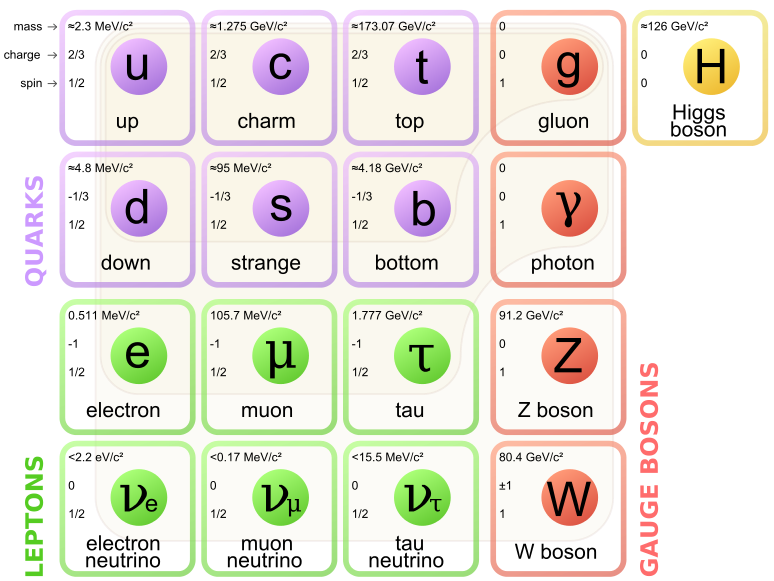
\includegraphics[width=0.7\textwidth]{figures/Standard_Model_of_Elementary_Particles.png}
\caption{The standard model of particle physics where the three first columns represent the so called generations, starting with the first. \cite{33wiki1:Online}}
\label{fig:standardModel}
\end{figure}

\if{0}
Made it su2  because? SM is based on it but why? Number of particles?

Why only left doublets and right singlets? Did they know? Massless particles? From isospin in strong?

The elementary particles are arranged as doublets for chiral left-handed fields and singlets for right-handed fields in the form.

\begin{equation}
\begin{pmatrix}
    u\\
    d'
\end{pmatrix}_L
\begin{pmatrix}
    c\\
    s'
\end{pmatrix}_L
\begin{pmatrix}
    t\\
    b'
\end{pmatrix}_L
\begin{pmatrix}
    e\\
    \nu_e
\end{pmatrix}_L
\begin{pmatrix}
    \mu\\
    \nu_\mu
\end{pmatrix}_L
\begin{pmatrix}
    \tau\\
    \nu_\tau
\end{pmatrix}_L
\end{equation}
and $u_R$,  $d_R$, $s_R$, $c_R$, $b_R$, $t_R$, $e_R$, $\mu_R$, $\tau_R$. 
Note how the neutrino is not modelled with a right handed component as the existence of right handed neutrinos was ruled out by \textbf{EXPERIMENT} before this theory was designed.

More details
\fi

\pagebreak

\section{Neutrino interactions}\label{subsection:Neutrino interactions}
The described theory can be used to describe how neutrinos interact and with what.

Neutrino interactions are split into two different types depending on which boson mediates the interaction.
Charge Current (CC) interactions change the final state quarks or leptons by one unit of electric charge and are mediated by the $W^+$ and $W^-$ bosons while Neutral Current (NC) interactions do not change the charge and are mediated by a $Z^0$ boson. 
To look at possible interactions of neutrinos described in the Standard Model of particle physics, one needs to look at the quantum field theory description of the interactions\cite{3Peskin, 2Hallsjo}.  The further subsections have been split depending on what interaction particle is involved.

\subsection{Neutrino-electron interactions}

%\textbf{New material}

Through the theory it is clear that neutrinos should interact with electrons. Electrons are a fundamental particle meaning that the interaction can be seen as pointlike interactions.

When it comes to neutrino and electron interactions, experimentally only the following have been observed:

Lagrangian for NC scattering, $\nu_x y \rightarrow \nu_x y$:
\begin{equation}
\mathcal{L}=-\frac{G_F}{\sqrt{2}} \left[ \bar{\nu_x}\gamma_\alpha (1-\gamma_5)\nu_x \right] \left[ \bar{y} \gamma_\alpha (g_V-g_A \gamma_5)y \right]
\end{equation}

with the constants as defined previously. The Fermi constant $G_F$, the Wienberg angle $\theta_W$ and where $g_\nu$ and $g_A$ are constants relating to strong interactions from v-a theory.

Lagrangian for CC scattering, $\nu_x y \rightarrow \nu_y x$:
\begin{equation}
\mathcal{L}=-\frac{G_F}{\sqrt{2}} \left[ \bar{\nu_x}\gamma_\alpha (1-\gamma_5)x\right] \left[ \bar{\nu_y}\gamma_\alpha (1-\gamma_5)y \right]
\end{equation}

From the Lagrangian the cross-sections are calculated by first calculating the  interaction amplitude by using the initial and final states to evaluate the Lagrangian. This amplitude can then be related to a derivative of the cross-section with can be integrated to provide the final cross-section. The details can be found in~\cite{3Peskin}.

The various processes involving an electron as an initial state with their calculated cross-sections can be seen in table~\ref{tab:electronproc} where the variable $s$ is the mandelstam variable, $s=(p_{\nu_\mu} + p_e)^2 = 2m_e E_{\nu_\mu}$

\begin{table}[h!]
\centering
\caption{Neutrino interactions with electrons}
\label{tab:electronproc}
\begin{tabular}{|l|l|l|}
 \hline
Type & Process & Cross-section \\
 \hline
CC interaction & $\nu_\mu + e^- \rightarrow \mu^- + \nu_e$  & $\frac{G_F^2 s}{\pi}$\\
CC+NC Scattering & $\nu_e + e^- \rightarrow \nu_e + e^-$ & $\frac{G_F^2 s}{4\pi} \left[ (2\sin^2 \theta_W -1){}^2 +\frac{4}{3}\sin^2 \theta_W \right]$\\ 
CC+NC Scattering & $\bar{\nu_e} + e^- \rightarrow \bar{\nu_e} + e^-$ & $\frac{G_F^2 s}{4\pi} \left[ \frac{1}{3}(2\sin^2 \theta_W +1){}^2 +4\sin^2 \theta_W \right]$ \\
NC Scattering & $\nu_\mu + e^- \rightarrow \nu_\mu + e^-$ & $\frac{G_F^2 s}{4\pi} \left[ (2\sin^2 \theta_W -1){}^2 +\frac{4}{3}\sin^2 \theta_W \right]$ \\
NC Scattering & $\bar{\nu_\mu} + e^- \rightarrow \bar{\nu_\mu} + e^-$ &$\frac{G_F^2 s}{4\pi} \left[ \frac{1}{3}(2\sin^2 \theta_W -1){}^2 +4\sin^2 \theta_W \right]$ \\
Neutrino pair production & $e^+ + e^- \rightarrow \nu_e + \bar{\nu_e}$ & $\frac{G_F^2 s}{12\pi} \left[ \frac{1}{2} + 2\sin^2 \theta_W + 4\sin^4 \theta_W \right]$ \\
Neutrino pair production & $e^+ + e^- \rightarrow \nu_\mu + \bar{\nu_\mu}$ & $\frac{G_F^2 s}{12\pi} \left[ \frac{1}{2} - 2\sin^2 \theta_W + 4\sin^4 \theta_W \right]$ \\
 \hline
\end{tabular}
\end{table}

To make it simpler for calculations and visualization these interactions have been plotted as Feynman diagrams in~\FigRef{fig:einteractions1}, \FigRef{fig:einteractions2} and \FigRef{fig:einteractions3}.

\begin{figure}[h!]
\vspace{2mm}
\centering
\begin{subfigure}{.5\textwidth}
  \centering
  \begin{fmffile}{TEST}
\begin{fmfgraph*}(120,80)
\fmfstraight
\fmfleft{i1,i2}
\fmfright{o1,o2}

\fmf{fermion}{i1,v1,o1}
%\fmf{fermion}{v1,o1}
\fmf{fermion}{i2,v2,o2}
\fmf{boson,label=$W^-$}{v1,v2}
%\fmf{fermion}{o2,v2}
%\fmf{fermion}{v2,o3}
\fmflabel{$e^{-}$}{i1}
\fmflabel{$\nu_{\mu}/\nu_{e}/\nu_{\mu}$}{i2}
\fmflabel{$\nu_{e}/\nu_{\mu}/\nu_{\mu}$}{o1}
\fmflabel{$\mu^-/e^-/e^-$}{o2}
\end{fmfgraph*}
\end{fmffile}
\end{subfigure}%
\begin{subfigure}{.5\textwidth}
  \centering
  \begin{fmffile}{TEST2}
\begin{fmfgraph*}(120,80)
\fmfstraight
\fmfleft{i1,o1}
\fmfright{i2,o2}

\fmf{fermion}{v1,o1}
\fmf{fermion}{i1,v1}

\fmf{boson,label=$W^+$}{v1,v2}
\fmf{fermion}{i2,v2}
\fmf{fermion}{v2,o2}

\fmflabel{$e^{-}$}{i1}
\fmflabel{$\bar{\nu_e}$}{o1}
\fmflabel{$\bar{\nu_e}$}{i2}
\fmflabel{$e^{-}$}{o2}
\end{fmfgraph*}
\end{fmffile}
\end{subfigure}
\vspace{2mm}
\caption{Charge interaction between neutrinos and electrons}
\label{fig:einteractions1}
\end{figure}

\begin{figure}[h!]
\centering
\begin{subfigure}{.5\textwidth}
  \centering
  \begin{fmffile}{TEST3}
\begin{fmfgraph*}(120,80)
\fmfstraight
\fmfleft{i1,i2}
\fmfright{o1,o2}

\fmf{fermion}{i1,v1,o1}
%\fmf{fermion}{v1,o1}
\fmf{fermion}{i2,v2,o2}
\fmf{boson,label=$Z^0$}{v1,v2}
%\fmf{fermion}{o2,v2}
%\fmf{fermion}{v2,o3}
\fmflabel{$e^{-}$}{i1}
\fmflabel{$\nu_{e}/\nu_{\mu}$}{i2}
\fmflabel{$\nu_{e}/\nu_{\mu}$}{o2}
\fmflabel{$e^-$}{o1}
\end{fmfgraph*}
\end{fmffile}
\end{subfigure}%
\begin{subfigure}{.5\textwidth}
  \centering
  \begin{fmffile}{TEST4}
\begin{fmfgraph*}(120,80)
\fmfstraight
\fmfleft{i1,i2}
\fmfright{o1,o2}

\fmf{phantom}{i1,v1,o1}
\fmf{phantom}{i2,v2,o2}
\fmf{fermion}{i1,v1}
\fmf{fermion}{o1,v1}
\fmf{fermion}{i2,v2}
\fmf{fermion}{v2,o2}

\fmf{boson,label=$Z^0$}{v1,v2}
%\fmf{fermion}{o2,v2}
%\fmf{fermion}{v2,o3}
\fmflabel{$e^{-}$}{i1}
\fmflabel{$\bar{\nu_{\mu}}/\bar{\nu_{e}}$}{i2}
\fmflabel{$\bar{\nu_{\mu}}/\bar{\nu_{e}}$}{o2}
\fmflabel{$e^{-}$}{o1}
\end{fmfgraph*}
\end{fmffile}
\end{subfigure}
\vspace{2mm}
\caption{Neutral interaction between neutrinos and electrons}
\label{fig:einteractions2}
\end{figure}

\begin{figure}[h!]
\centering
\begin{subfigure}{.5\textwidth}
  \centering
  \begin{fmffile}{TEST5}
\begin{fmfgraph*}(120,80)
\fmfstraight
\fmfleft{i1,i2}
\fmfright{o1,o2}


\fmf{phantom}{i1,v1,o1}
\fmf{phantom}{i2,v2,o2}
\fmf{fermion}{i1,v1}
\fmf{fermion}{v1,o1}
\fmf{fermion}{v2,i2}
\fmf{fermion}{o2,v2}

%\fmf{fermion}{i1,v1,o1}
%\fmf{fermion}{v1,o1}
%\fmf{fermion}{i2,v2,o2}
\fmf{boson,label=$W^\pm$}{v1,v2}
%\fmf{fermion}{o2,v2}
%\fmf{fermion}{v2,o3}
\fmflabel{$e^{-}$}{i1}
\fmflabel{$e^+$}{i2}
\fmflabel{$\bar{\nu_{e}}$}{o2}
\fmflabel{$\nu_e$}{o1}
\end{fmfgraph*}
\end{fmffile}
\end{subfigure}%
\begin{subfigure}{.5\textwidth}
  \centering
  \begin{fmffile}{TEST6}
\begin{fmfgraph*}(120,80)
\fmfstraight
\fmfleft{i1,o1}
\fmfright{i2,o2}

\fmf{fermion}{v1,o1}
\fmf{fermion}{i1,v1}

\fmf{boson,label=$Z^0$}{v1,v2}
\fmf{fermion}{i2,v2}
\fmf{fermion}{v2,o2}

\fmflabel{$e^{-}$}{i1}
\fmflabel{$e^+$}{o1}
\fmflabel{$\bar{\nu_e}$}{i2}
\fmflabel{$\nu_e$}{o2}
\end{fmfgraph*}
\end{fmffile}
\end{subfigure}
\vspace{2mm}
\caption{Neutrino pair production}
\label{fig:einteractions3}
\end{figure}


\if{0}
\begin{figure}[h!]
  \centering
  \begin{fmffile}{TEST2}
\begin{fmfgraph*}(120,80)
\fmfstraight
\fmfleft{i1,i2}
\fmfright{o1,o2}


\fmf{phantom}{i1,v1,o1}
\fmf{phantom}{i2,v2,o2}
\fmf{fermion}{i1,v1}
\fmf{fermion}{o1,v1}
\fmf{fermion}{v2,i2}
\fmf{fermion}{v2,o2}

%\fmf{fermion}{i1,v1,o1}
%\fmf{fermion}{v1,o1}
%\fmf{fermion}{i2,v2,o2}
\fmf{boson,label=$Z^+$}{v1,v2}
%\fmf{fermion}{o2,v2}
%\fmf{fermion}{v2,o3}
\fmflabel{$e^{-}$}{i1}
\fmflabel{$\bar{\nu_{\mu}}/\bar{\nu_{e}}$}{i2}
\fmflabel{$\bar{\nu_{\mu}}/\bar{\nu_{e}}$}{o1}
\fmflabel{$e^-/e^-$}{o2}
\end{fmfgraph*}
\end{fmffile}
\vspace{2mm}
\caption{TEST2}
\label{fig:test2}
\end{figure}
\fi

\subsection{Neutrino-quark scattering}
Moving away from electrons into quarks one has to take into account that quarks are always bound in a hadron, and thus do not exist in a free state. 

Neutrino-quark interactions can be understood in two different ways. Starting with inverse beta-decay where a proton interacts with an anti-neutrino producing a positron and neutrino, $\bar{\nu_e}+p \rightarrow e^+ + n$, can be seen as an interaction where the full hadron interacts and only changes its weak charge instead of seeing each quark interact separately. The interacting particle, proton changes into another baryon the neutron. However at higher energies it is possible for the quark to become ejected from the proton and the interaction changing the proton from a baryon into a meson.

%Could use muon neutrino instead? $\nu_\mu + n \rightarrow \mu^- + p$

\subsubsection{Quasi-elastic interactions}
Quasi-elastic relates to when the neutrino interacts with the proton as a whole. 
This however requires some factors for modelling the nucleus as a whole, compared to the electron which was seen as point-like. The cross section is given as:
\begin{equation}
\sigma(\bar{\nu_e} + p \rightarrow e^+ + n) = \frac{G_Fs}{\pi} \times \cos^2 \theta_C \times \xi_{mass} \times (g^2_v + 3 g^2_A)
\end{equation}
with corrections for charge-current quark mixing transition from u to d quark $( \cos^2 \theta_C)$, a mass suppression factor $\xi_{mass}$ and proton form factors $g^2_v + 3 g^2_A$ ~\cite{47Soler}.

It is also interesting to note that apart from inverse beta-decay which is a CC interaction, an Quasi-elastic NC interaction can also happen $\nu_\mu + p \rightarrow \nu_\mu + p$ which knocks on the proton but does not change it.

%Inverse beta decay. Details of how we model the proton as similar to an electron with magnetic moment, 
%Both charge current and neutral current. relate to electron scattering and explain 2p2h and other resent models.
%No longer point like, no free quarks, require parton models etc etc. nu N Elastic scattering
%Can do beta decay without to many changes. Still nucleus after interaction.
%Plot showing that this is interesting below or around 1 GeV? Write about transition region.Also neutral CCQE!$\nu_\mu + p \rightarrow \nu_\mu + p$

\subsubsection{Deep inelastic scattering}
If the neutrino has an energy of around or above 1 GeV there is enough energy that the neutrino can break up the nucleon and interact with the quarks as if they were free particles. It becomes quite difficult to calculate the cross-section for these interactions as it depends on the final particle(s) as well as understanding the so called form factors relating the quarks to the proton. 
DIS comes with both a charge current and neutral current modes as $\nu_\mu + p \rightarrow \mu^- + X$ or $\nu_\mu + p \rightarrow \nu_\mu + X$.

More details can be found in~\cite{47Soler}.

\subsubsection{Resonant interactions}
Between the elastic and inelastic region is an area associated with pion production through the excitation of baryon resonances, $\nu_i + N \rightarrow l + N*$ where the nucleus further decays $N* \rightarrow \pi + N'$. Two examples with delta particles can be seen below.
\begin{align}
\nu_\mu + N &\rightarrow \mu^- + \Delta^{++} \rightarrow \mu^- + p + \pi^+\\
\nu_\mu + N &\rightarrow \mu^- + \Delta^{+} \rightarrow \mu^- + n + \pi^+
\end{align}

\subsection{Comparing neutrino interactions to QED}
%Bitten of too much?Quickly introduce the different parts, center of mass energy, fermi coupling, weinbarg angle and their importance for the comparison.
\if{0}
As discussed previously, neutrino interactions in the SM are described by the weak interaction model. Through initial experimental studies, the model was thought to not have any gauge boson and be described by the Lagrangian density $\mathscr{L} = -\frac{G_F}{\sqrt{2}} j_\mu ^\dagger j^\mu$ where $G_F$ is the Fermi constant $\approx 1.17 \times 10^{-5} GeV^{-2}$ and $j_\mu$ is the weak V-A current \cite{47Soler}. This gives a good approximation for rates in weak processes but is a non-renormalizable theory. The solution for this is to introduce a massive vector boson drawn in \FigRef{fig:beta} but not yet named as a W boson. Introducing these massive vector bosons leads to some interesting consequences since at this time only Quantum ElectroDynamics (QED) had been described with a non-massive boson, the photon. Introducing the photon into this theory and producing a unified electroweak theory, coupling isospin $g$ and weak hypercharge $g^\prime$, as well as providing the problem of describing how bosons can have mass. It was this unification which was one of the bases of SM and the problem of masses introduces spontaneous symmetry breaking which is part of the Higgs mechanism. In electroweak theory there are in total four bosons, two massive and charged, one massive chargeless and one massless and chargeless. these are denoted as $W^+, W^-, Z^0, \gamma$. The theoretical relationship between the mass of $W$ and $Z^0$ is $m_W = m_Z \cos \theta_W$ where $\theta_W$ is the Weinberg angle.

Neutrino interactions are split into two different types depending on which boson mediates the interaction.
Charge Current (CC) interactions change the final state quarks or leptons by one unit of electric charge and are mediated by the $W^+$ and $W^-$ bosons while Neutral Current (NC) interactions do not change the charge and are mediated by a $Z^0$ boson. 
To look at possible interactions of neutrinos described in the Standard Model of particle physics, one needs to look at the quantum field theory description of the interactions\cite{3Peskin, 2Hallsjo}. Sample Feynman diagrams showing these interactions can be seen in \FigRef{fig:CC} and \FigRef{fig:NC}.

\begin{figure}[h!]
\centering
\begin{subfigure}{.5\textwidth}
  \centering
  \begin{fmffile}{W+}
\begin{fmfgraph*}(120,80)
\fmfstraight
\fmfleft{i1,i2,o1}
\fmfright{o2,o3}

\fmf{fermion}{v1,i1}
\fmf{fermion}{o1,v1}

\fmf{boson,label=$W^{+}$}{v1,v2}
\fmf{fermion}{o2,v2}
\fmf{fermion}{v2,o3}

\fmflabel{$\bar{d}$}{i1}
\fmflabel{u}{o1}
\fmflabel{$e^{+}$}{o2}
\fmflabel{$\nu_e$}{o3}
\end{fmfgraph*}
\end{fmffile}
  %\caption{A subfigure}
  %\label{fig:sub1}
\end{subfigure}%
\begin{subfigure}{.5\textwidth}
  \centering
  \begin{fmffile}{W-}
\begin{fmfgraph*}(120,80)
\fmfstraight
\fmfleft{i1,i2,o1}
\fmfright{o2,o3}

\fmf{fermion}{i1,v1}
\fmf{fermion}{v1,o1}

\fmf{boson,label=$W^{-}$}{v1,v2}
\fmf{fermion}{v2,o2}
\fmf{fermion}{o3,v2}

\fmflabel{d}{i1}
\fmflabel{$\bar{u}$}{o1}
\fmflabel{$e^{-}$}{o2}
\fmflabel{$\bar{\nu}_e$}{o3}
\end{fmfgraph*}
\end{fmffile}
  %\caption{A subfigure}
  %\label{fig:sub2}
\end{subfigure}
\vspace{2mm}
\caption{Feynman diagrams showing an example of a charge current interaction.}
\label{fig:CC}
\end{figure}

\begin{figure}[h!]
\centering
  \begin{fmffile}{Z}
\begin{fmfgraph*}(120,80)
\fmfstraight
\fmfleft{i1,i2}
\fmfright{o1,o2}

\fmf{fermion}{i1,v1,o1}
%\fmf{fermion}{v1,o1}

\fmf{fermion}{i2,v2,o2}

\fmf{boson,label=$Z^{0}$}{v1,v2}
%\fmf{fermion}{o2,v2}
%\fmf{fermion}{v2,o3}

\fmflabel{$e^{-}$}{i1}
\fmflabel{$\nu_{\mu}$}{i2}
\fmflabel{$e^{-}$}{o1}
\fmflabel{$\nu_{\mu}$}{o2}
\end{fmfgraph*}
\end{fmffile}
  %\caption{A subfigure}
  %\label{fig:sub1}

\vspace{2mm}
\caption{Feynman diagram showing an example of a neutral current interaction.}
\label{fig:NC}
\end{figure}

From the Feynman diagrams one can calculate the probability of the interaction occurring, details can be found in \cite{3Peskin} among others.

\fi

It is interesting to compare the probability for Charge Current and Neutral Current interactions with the equivalent QED or electromagnetic interactions. In  \FigRef{fig:weakQED} a comparison is made between QED and a weak interaction with the same initial and final states. Calculating the cross-sections when $E<<M_Z$ the following quotient is produced: $\frac{\sigma_{Weak}}{\sigma_{QED}} \approx (\frac{s}{M_Z^2})^2$ where s is the square of the center of mass energy, $M_Z$ is the mass of the Z-boson. Currently the Z-boson mass is $91.1876 GeV$~\cite{13PDG} but since s varies it is hard to give a value to the quotient. For the energy range where $E<<M_Z$ this quotient varies from $0.01 \rightarrow 0.1225$. With the current values QED is approximately 100 times more likely to occur than a weak interaction..

\begin{figure}[h!]
\centering
\begin{subfigure}{.5\textwidth}
  \centering
  \begin{fmffile}{QED}
\begin{fmfgraph*}(120,80)
\fmfstraight
\fmfleft{i1,i2,o1}
\fmfright{o2,o3}

\fmf{fermion}{v1,i1}
\fmf{fermion}{o1,v1}

\fmf{boson,label=$\gamma$}{v1,v2}
\fmf{fermion}{o2,v2}
\fmf{fermion}{v2,o3}

\fmflabel{$e^{+}$}{i1}
\fmflabel{$e^{-}$}{o1}
\fmflabel{$\bar{f}$}{o2}
\fmflabel{$f$}{o3}
\end{fmfgraph*}
\end{fmffile}
  %\caption{A subfigure}
  %\label{fig:sub1}
\end{subfigure}%
\begin{subfigure}{.5\textwidth}
  \centering
  \begin{fmffile}{Weak}
\begin{fmfgraph*}(120,80)
\fmfstraight
\fmfleft{i1,i2,o1}
\fmfright{o2,o3}

\fmf{fermion}{v1,i1}
\fmf{fermion}{o1,v1}

\fmf{boson,label=$Z^0$}{v1,v2}
\fmf{fermion}{o2,v2}
\fmf{fermion}{v2,o3}

\fmflabel{$e^{+}$}{i1}
\fmflabel{$e^{-}$}{o1}
\fmflabel{$\bar{f}$}{o2}
\fmflabel{$f$}{o3}
\end{fmfgraph*}
\end{fmffile}
  %\caption{A subfigure}
  %\label{fig:sub2}
\end{subfigure}
\vspace{2mm}
\caption{The QED and the weak contributions to the scattering electron-positron to any quark or lepton pair.\protect\footnotemark}
\label{fig:weakQED}
\end{figure}
\footnotetext{If $f=e^-$ a T-channel diagram has to be added as well} 

The CC and NC examples in  \FigRef{fig:CMPNCCC} with electrons and muon neutrinos, so that the final states can be distinguished, the cross sections of both can be written as $\sigma_{CC} (\nu_\mu e^-) \approx \frac{G_F^2 s}{\pi} $ and $\sigma_{NC} (\nu_\mu e^-) \approx \frac{G_F^2 s}{\pi} \left[ (-\frac{1}{2} + \sin^2 \theta_W)^2 + \frac{1}{3}\sin^4 \theta_W\right] $ where $G_F$ and $\theta_W$ are defined above. This gives a relation CC and NC as $\frac{\sigma_{CC}}{\sigma_{NC}} = 1/\left[ (-\frac{1}{2} + \sin^2 \theta_W)^2 + \frac{1}{3}\sin^4 \theta_W\right] \approx 11$. With the current values CC is approximately 11 times more likely to occur than NC.

\begin{figure}[h!]
\centering
\begin{subfigure}{.5\textwidth}
  \centering
  \begin{fmffile}{ECC}
\begin{fmfgraph*}(120,80)
\fmfstraight
\fmfleft{i1,i2}
\fmfright{o1,o2}

\fmf{fermion}{i1,v1,o1}
%\fmf{fermion}{v1,o1}

\fmf{fermion}{i2,v2,o2}

\fmf{boson,label=$W^-$}{v1,v2}
%\fmf{fermion}{o2,v2}
%\fmf{fermion}{v2,o3}

\fmflabel{$e^{-}$}{i1}
\fmflabel{$\nu_{\mu}$}{i2}
\fmflabel{$\nu_{e}$}{o1}
\fmflabel{$\mu^-$}{o2}
\end{fmfgraph*}
\end{fmffile}
  %\caption{A subfigure}
  %\label{fig:sub1}
\end{subfigure}%
\begin{subfigure}{.5\textwidth}
  \centering
  \begin{fmffile}{ENC}
\begin{fmfgraph*}(120,80)
\fmfstraight
\fmfleft{i1,i2}
\fmfright{o1,o2}

\fmf{fermion}{i1,v1,o1}
%\fmf{fermion}{v1,o1}

\fmf{fermion}{i2,v2,o2}

\fmf{boson,label=$Z^{0}$}{v1,v2}
%\fmf{fermion}{o2,v2}
%\fmf{fermion}{v2,o3}

\fmflabel{$e^{-}$}{i1}
\fmflabel{$\nu_{\mu}$}{i2}
\fmflabel{$e^-$}{o1}
\fmflabel{$\nu_{\mu}$}{o2}
\end{fmfgraph*}
\end{fmffile}
  %\caption{A subfigure}
  %\label{fig:sub2}
\end{subfigure}
\vspace{2mm}
\caption{Feynman diagrams, CC(Left) and NC(Right) with the same initial states.}
\label{fig:CMPNCCC}
\end{figure}

\pagebreak
\section{Missing neutrinos}\label{subsection:Missing}

The sun generate energy principally through the proton-proton chain reaction~\cite{48Solar}. In this chain electron neutrino are produced through proton-proton interactions and beta decay processes. 
\begin{equation}
\label{eq:ppreaction}
\ce{H^+ + H^+ ->  ^{2}H + e^+ + $\nu_e$  }
\end{equation}
The proton-proton interaction has the highest flux, $6.1 \times 10^{10} cm^{-2} sec^{-1}$ but produces neutrinos at very low energies  ($<0.4 MeV$) making them difficult to detect. 
Further on in this chain a Boron decay,
% {}^8_5B \rightarrow {}^9_4 Be + e^+ + \nu_e
\begin{equation}
\label{eq:BoronDecay}
\ce{^8B -> ^4He + ^4He + $\nu_e$}
\end{equation}
produces electron neutrinos with energies up to 18 MeV, however the fluxes are much lower than proton-proton interactions, $3.2 \times 10^6 cm^{-2} sec^{-1}$. Neutrinos in this energy can be used in inverse-beta decay transforming chlorine into argon.
%\nu_e + {}^{37} Cl \rightarrow {}^{37} Ar + e^-
\begin{equation}
\ce{$\nu_e$ + ^{37}Cl -> ^{37}Ar + $e^{-}$ }
\end{equation}
The amount of argon can then be counted by measuring x-rays comming from the decaying argon isotope and related to the neutrino flux. The Homestake experiment used this technique ran from 1970 until 1994 with a goal to measure the flux of electron neutrinos. They measured the flux of electron neutrinos and found only around 1/3, (1.75/4.7), of the expected value from the theoretical model of the nuclear reactions in the core of the sun \cite{9Davis}. 

This results shock the whole neutrino field by suggesting something fundamentally wrong in the understanding of the neutrino, either in the interactions or in the solar model. There were various solar experiments which confirmed the solar neutrino model~\cite{48Solar} implying something wrong in the interaction model. At the same time measurements were performed at several other detectors, Sudbury Neutrino Observatory (SNO)~\cite{Fix6}, Kamiokande~\cite{55Kamiokande} and Super-Kamiokande~\cite{10Fukuda} all in agreement with a lesser flux. Further information from the measurement at SNO hinted at the fact that additional neutrino flavours may be produced, contradicting the verified solar neutrino model. One of the possible explanations for the deficit was neutrino oscillations proposed by Bruno Pontecorvo~\cite{11Pontecorvo}. 

The oscillation model is in good agreement with experimental values and was verified at SNO and Super-Kamiokande awarding the neutrino flavour oscillation measurements with Nobel prizes in 2015 and paved the way for physics beyond the Standard Model. %\textbf{REFERENCE TO MENTIONING THEM IN CHAP 2}

\pagebreak
\section{Neutrino mass and oscillation in vacuum}\label{subsection:Neutrinomassandoscillation}
While looking at an analog of neutral kaon mixing for neutrinos Bruno Pontecorvo, in 1957, developed the concept of neutrino-antineutrino transitions~\cite{11Pontecorvo}. Even though to date no matter-antimatter oscillation had been observed, the concept formed the foundation of lepton mixing, which was developed by Maki, Nakagawa, and Sakata~\cite{12Maki} and refined into a neutrino flavour oscillation model by Bruno Pontecorvo. They managed to show that neutrino mixing is a natural outcome of adding neutrino mass to a gauge theory~\cite{11Pontecorvo}

The relation between the flavour and mass eigenstates can be expressed as,
\begin{equation}
\label{eq:eigenstates}
 \left| \nu_\alpha \right\rangle = \sum_{i} U^{*}_{\alpha i} \left| \nu_i \right\rangle,
 \left| \bar{\nu_\alpha} \right\rangle = \sum_{i} U_{\alpha i} \left| \bar{\nu_i} \right\rangle\
 \end{equation}
where
 $\left| \nu_\alpha \right\rangle $ is a neutrino with a fixed flavour, $\alpha$ is one of \{e,$\mu$,$\tau$\} and  $\left| \nu_i \right\rangle$ is a neutrino with a fixed mass.
$U$ is the Pontecorvo-Maki-Nagawa-Sakata (PMNS) matrix in \eqref{PMNS},
\begin{equation}
\label{PMNS}
\begin{aligned}
U ={} & 
 \begin{pmatrix}
 c_{12} & s_{12} & 0\\
  -s_{12} & c_{12} & 0\\
  0 & 0 & 1\\
 \end{pmatrix} 
  \begin{pmatrix}
 1 & 0 & 0\\
  0 & c_{23} & s_{23}\\
  0 & -s_{23} & c_{23}\\
 \end{pmatrix} 
   \begin{pmatrix}
 c_{13} & 0 & s_{13}e^{i\delta_{CP}}\\
  0 & 1 & 0\\
  -s_{13}e^{-i\delta_{CP}} & 0 & c_{13}\\
 \end{pmatrix} 
 \\
 & \times
  \begin{pmatrix}
1 & 0& 0\\
  0 & e^{i\phi_2} & 0\\
  0 & 0 & e^{i\phi_3}\\
 \end{pmatrix} 
 \end{aligned}
\end{equation}
where $s_{ij} = \sin\theta_{ij}$ and $c_{ij} = \cos\theta_{ij}$ with $\theta_{ij}$ the three mixing angles and $\delta_{CP}$, $\phi_2$ and $\phi_3$ are complex phases. The parameters $\phi_2$ and $\phi_3$ are only non-zero if neutrinos are their own antiparticles, denoted as Majorana, which is still unknown at the time of writing this~\cite{13PDG}. This would be an interesting result as it would imply a splitting with the relation to the Higgs field. The three first matrices are denoted the Dirac part of the PMNS matrix and the final forth matrix is the Majorana term which is non-identity only if neutrinos are Majorana.

The probability of finding a neutrino in a specific time-dependent state is related to the mass states through the PMNS matrix elements and the time-evolution operator. The PMNS introduces a rotation in the space of mass eigenstates. The derivations of the oscillation probability for two-neutrino and three-neutrino oscillations can be found in the literature \cite{34doi:10.1142/9789812562203_0002}. The three neutrino flavour state shown in equation \ref{eq:eigenstates} evolves as a function of time as:
%The interpretation is similar to that of a time-dependent quantum state, the probability of finding a neutrino in a specific state is related to the mass states through the PMNS matrix in which the elements are time dependent.
%It can also be thought of as a rotation in space. The derivations of the oscillation probability for assuming only two neutrinos and also for three neutrinos are often given in literature for instance it is given in . The three neutrino flavour state \ref{eq:eigenstates} in an initial beam evolves in time as:

\begin{equation}
\label{eq:eigenstatesTime}
 \left| \nu_\alpha (t) \right\rangle = \sum_{i} e^{-i E_i t} U_{\alpha i} \left| \nu_i \right\rangle\,
 \end{equation}

which gives the probability of flavour evolution as 
\begin{equation}
\begin{aligned}
P_{\nu_\alpha \rightarrow \nu_\beta} (t) &= \left|  \langle \nu_\beta \left| \nu_\alpha     \right\rangle  \right|^2
& = \sum_{i,j} \left| U_{\alpha i} U_{\beta i}^* U{\alpha j}^* U_{\beta j} \right| \cos[(E_i - E_j)t -arg(U_{\alpha i} U_{\beta i}^* U{\alpha j}^* U_{\beta j} ) ]
\end{aligned}
\end{equation}

\begin{equation}
\label{eq:Energy-momentum}
E_\alpha = \sqrt{\vec{p}^2 + m_i^2} \approx \left| \vec{p} \right| + \frac{m_i^2}{2\left| \vec{p} \right|}
\end{equation}

If one has a beam of neutrinos in an initial flavour state $|\nu_\alpha \rangle$, the probability to find the neutrinos changing to flavour state $|\nu_\beta \rangle$, after a distance $x$, is given by
%Which can then be rewritten to depend on distance travelled by the beam (x) if using a relativistic approximation of the   as

\begin{equation}
\label{eq:Problength}
\begin{aligned}
P_{\nu_\alpha \rightarrow \nu_\beta} (x) &= \left|  \langle \nu_\beta \left| \nu_\alpha     \right\rangle  \right|^2
& = \sum_{i,j} \left| U_{\alpha i} U_{\beta i}^* U{\alpha j}^* U_{\beta j} \right| \cos\left[\frac{2\pi x}{L_{ij}} -arg(U_{\alpha i} U_{\beta i}^* U_{\alpha j}^* U_{\beta j} ) \right],
\end{aligned}
\end{equation}
where the approximate energy-momentum relationship of equation \ref{eq:Energy-momentum} has been taken into account, where the oscillation length is given by $L_{ij} = \frac{4\pi  \left| \vec{p} \right| }{\left| m_i^2 - m_j^2 \right|}=\frac{4\pi  \left| \vec{p} \right| }{\left| \Delta m_{ij}^2 \right|} $ and $\vec{p}$ is the 3-momentum of the neutrinos in the initial beam.

If is worth noting that the equation can be simplified assuming only oscillation into one flavour:
\begin{equation}
P_{\nu_\mu \rightarrow \nu_y} (x) = \sin^2(2\theta_{\mu y})\sin^2 \left( \frac{1.27\Delta m_{\mu y}^2 x}{E_\nu} \right)
\label{eq:twoPNeutrinoosc}
\end{equation}
where $1.27$ is a unit constant which comes when $\Delta m^2$ is given in units of $eV^2$, $x$ in meters and $E_\nu$ is $MeV$.

The mass-squared difference between neutrino mass states $\left|m_i^2 - m_j^2\right|$ has to be different from zero for there to be neutrino oscillations, so at least one of the neutrinos must have non-zero mass which currently is not explained through the Standard Model. Furthermore, if the elements of the PMNS matrix $U_{\alpha i}$ are all real then $arg(U_{\alpha i} U^*_{\beta i} U^*_{\alpha j}  U_{\beta i} ) = 0$ and the CP-violating phase $\delta_{CP} =0$. The current experimental focus lies with trying to measure values for all these parameters. Current values of the neutrino masses can be found in table \ref{table:UpperNMass}

Looking at the oscillation probability \eqref{eq:Problength} two main classes of experiments for neutrino oscillations can be devised. Finding a distance $x$ to the source where $P_{\nu_\alpha \rightarrow \nu_\alpha} (x) < 1$, it is possible to look at so called disappearance of the beam by comparing the expected neutrino flux to the observed. For the disappearing flavour there must be a probability, $P_{\nu_\alpha \rightarrow \nu_\beta} (x) > 0, \alpha=\beta$ for another flavour to appear. The second kind of experiment, denoted as appearance, is based on looking for interaction products which are impossible without oscillations.  An example of this would be to see a positron from a muon neutrino beam. More on this can be found well described in~\cite{34doi:10.1142/9789812562203_0002} and examples of different detectors will be discussed in chapter~\ref{c:expIntro}. As a rule of thumb this L has to be on the order of km for energy ranges between MeV to GeV. This means that oscillations will have a small effect on short scale neutrino interactions measured close to the source.

Charge conjugation and parity (C and P, CP) symmetry states that physics should be the same for particles and anti-particles while the spatial coordinates are inverted. If $\delta_{CP}$ is non-zero it would imply CP symmetry is violated it would imply a difference between the rate of neutrino and anti-neutrino oscillations and could be responsible for the matter-antimatter asymmetry of the early universe. Current best-fit values (at 90\% confidence limit) have $\delta_{CP} = -1.79\pm 1.42$ for normal mass ordering and $\delta_{CP} = -1.41\pm 0.68$ for inverted mass ordering both rejecting the null hypothesis for $\delta_{CP}$ at around $3\sigma$\cite{T2KResults}.

%\textbf{ How does the formula look like and what changes in both orderings?} 

%Also that if $U_{\alpha i}$ is real, which is related to $\delta_{CP} = 0$, then $arg(U_{\alpha i} U_{\beta i}^* U_{\alpha j}^* U_{\beta j} ) = 0$.
%It can be seen that if $m_i^2 - m_j^2 = 0 $ this probability becomes $0$ which contradicts the experimental results. This means that atleast one of the neutrinos 

%and one of the most interesting for understanding more about the Big Bang theory is the complex phase $\delta_{CP}$. This is known as the CP-violating phase which, if non-zero, would state that there is a difference between how normal and anti-neutrinos oscillate. \textbf{Experimental value so far of CP}

Table \ref{table:UpperNMass} provides the current mass limits for neutrinos, note that currently there is no lower limit since it is only known that at least two of the neutrinos must have mass.

\begin {table}[H]
\begin{center}
\begin{tabular}{ |c|c|c| } 
 \hline
 Particle & 95\% CL Mass limit (MeV) & 95\% CL Anti-particle mass limit (MeV) \\ 
  \hline
 $\nu_e$ & $<0.225$ & $<2 \cdot 10^{-3}$ \\ 
 $\nu_\mu$ & $<0.19$ & No Data \\ 
  $\nu_\tau$ & $< 18.2$ & No Data \\ 
 \hline

\end{tabular}
\end{center}
\caption{Current upper neutrino mass limits ~\cite{13PDG}}
\label{table:UpperNMass}
\end {table}

\pagebreak
\section{CP-violation, baryogenesis and leptogenesis}
According to the Big Bang theory, matter and anti-matter were created in equal amounts\cite{14Berry}. Through observations of the universe, much more matter has been found compared to anti-matter. This constitutes one of the major unsolved problems in physics, where is all the anti-matter? There has currently not been any sign of an annihilation horizon, where matter and anti-matter interact nor has there been any sign of this in the cosmic background radiation\cite{14Berry}. One direct measurement was AMS-01, (Alpha Magnetic Spectrometer),which measured the ratio of anti-helium to helium in the universe to be of the order of $10^{-6}$~\cite{15AMS1}. 

The follow-up experiment, AMS-02, which is operational in the International Space Station, confirmed these results and measured the antibaryon component of the universe to be $\sim 10^{-9}$ less that of baryons~\cite{16AMS2}. As of now our current models account this difference to be $O(1)$ thus a factor of $10^9$ too small\cite{49Matter}. This implies that there must be a yet unknown process to account for the difference.

There exist two approaches to explain the matter asymmetry of the universe. The first is baryogenesis which studies possible mechanisms to enhance the baryon-antibaryon asymmetry, and the second is leptogenesis, in which CP violation in leptons translates into a baryon asymmetry. Leptogenesis will be covered in this thesis as it relates to neutrinos also it should be added that there are theories which explain baryogenesis through leptogenesis.

If neutrinos violate CP by their oscillations being different for neutrinos and anti-neutrinos, this could explain the matter anti-matter imbalance that has been observed. CP-violation exists in the Standard Model but it cannot explain the observed difference~\cite{3Peskin}, and measurements of the CP-violation in neutrino oscillations have not yet been able to show any conclusive results~\cite{17Gonzalez}.

\subsection{Current theory of leptogenesis}
Andrei Sakharov proposed three necessary conditions that any baryon-generating interaction, which would produce matter antimatter imbalance, must satisfy~\cite{37Sakharov}. These conditions are:
\begin{itemize}
\item Baryon number violation.
\item C-and CP-violation.
\item Deviation from thermal equilibrium.
\end{itemize}

The first condition is very important in that it related cosmological models with models in particle physics. It also gives us a way to produce an excess of baryons over anti-baryons, as long as there is no reverse interaction, hence requiring the C violation. CP-violation is needed to counteract the balancing as well and finally out of thermal equilibrium to get around CPT-symmetry. As briefly mentioned previously the second condition is fulfilled in the SM, but not enough, and the third can always be satisfied.

In \cite{36CRC} a number of viable scenarios for baryogenesis are briefly discussed, for instance Grand Unified theories, heavy Majorana neutrinos and supersymmetry.

\pagebreak
\section{Current Theories to explain neutrino mass}
The problem with neutrino masses is that we only see left-handed neutrinos. The standard way for fermions to obtain a mass through interaction with the Higgs field is through a three point interaction involving a left-handed fermion, a right-handed fermion, and the Higgs field. With no right handed neutrinos, there is no way to form such interactions, which lead to a mass term after symmetry breaking. This leaves the exact mechanism by which neutrinos acquire mass a mystery. When SM was created neutrinos were assumed to be massless since they were only left-handed. There are three main reasons to why the neutrino mass must be zero in the SM:
\begin{itemize}
\item There is no renormalizable operator which allows for a neutrino mass without introducing either an additional Higgs particle or by introducing right-handed neutrinos, neither of which have currently been observed.

\item The current Higgs is an $SU(2)_L$ doublet, thus it requires fermions to have both chiral states to provide mass. It could be possible to introduce further Higgs particles which do not require this.

\item There are no right-handed neutrinos. Right-handed neutrinos could be introduces which would allow the current Higgs or any other current mechanism to provide mass. This is because the right-handed neutrino will be modeled as a singlet state in the extended-SM.
\end{itemize}

There are different ongoing searches to find all categories of solutions, higher-order operators (non-renormalizable), other Higgs particles (Non $SU(2)_L $ doublets) and right-handed neutrinos.

In this thesis the focus will be on introducing right-handed neutrinos. There are two main mass terms both related to the Higgs mechanism, the so called Dirac term and the Majorana term.

\subsection{Dirac neutrinos}
Naively introducing right-handed neutrinos makes an assumptions that neutrinos and anti-neutrinos are distinct particles, however since the neutrino is electrically neutral, this does not have to be the case.
 
Introducing right-handed neutrinos introduces particles which will not interact in the SM since the electroweak interaction model only couples to left handed neutrinos. Thus right-handed neutrinos are often denoted sterile neutrinos and only interact through gravity. This introduces sterile neutrinos as a possible candidate as dark matter. \cite{SterileDark, SUSYdark}

The main problems with this description is both that no right-handed neutrinos have been detected and that the observed neutrino mass measurement requires a weaker coupling for neutrinos compared to the other leptons.

Dirac neutrinos could be experimentally verified by finding neutrino being different to anti-neutrinos or by finding both right-handed neutrinos and left-handed neutrinos as different particles.

\subsection{Majorana neutrinos}
Removing the assumption that neutrinos and anti-neutrinos are distinct allows for a simplified model. Right handed neutrinos have to be produces to conserve lepton number conservation but not to introduce a mass mechanism. Majorana mass also has no equivalent for other leptons and could explain the the neutrino mass is so small. Majorana neutrinos would allow neutrinoless double beta decay\cite{NeuLess} as an experimental verification.

\subsection{Summary}
In this chapter the theory of neutrino interactions as well as a the history of neutrinos have been introduced. The current issues with neutrinos in the SM and open questions have been presented.

%==============================================================================
%\section{Thesis Statement}
%\label{c:intro:thesisstatement}

%This is a thesis statement. There are many like it, but this one is mine.




\chapter{Neutrino  experiments}
\label{c:expIntro}

\section{Introduction}
Since the discovery of the neutrino in 1956 by Reines and Cowan~\cite{6Reines} a multitude of neutrino experiments have tried to measure the properties of the different neutrino flavours. Since the Homestake experiment many other experiments have been run to measure neutrino oscillations and the mass of the neutrinos. A detailed description of these experiments is outside of the scope of this thesis, in this section a description into the main types and milestones will be presented.

Neutrino experiments are split into three different categories based on the primary neutrino source. Each type features its own advantages and issues.
The detector types are:
\begin{itemize}
\item Atmospheric
\item Solar
\item Accelerator
\item Reactor
\end{itemize}
Each will be described briefly before examples are given.

\section{Atmospheric}

As mentioned in section~\ref{subsection:Missing} neutrinos at low energy ranges ($<18 MeV$) are produced through nuclear interactions in stars. There are other cosmological phenomena which produce these neutrinos, and some searches are looking for signs of new physics in these signals. 

The Earth is constantly bombarded by cosmic-ray particles from space. When they hit the atmosphere, these high-energy protons interact with air molecules to produce showers of pions, which subsequently decay to muons and muon-neutrinos. This process is exactly similar to that used to produce neutrino beams from particle accelerators. Early observations of atmospheric neutrinos were contradictory, with some experiments observing approximately the expected ratio while others saw significantly fewer muon-neutrinos than expected, similar to the missing solar neutrinos, the Atmospheric Neutrino Anomaly. This was a measurement done by Super-Kamiokande and confirmed, together with the Homestake experiment, the existence of neutrino oscillations.

The atmosperhic neutrinos are produced from cosmic-rays interacting through nuclear interactions producing pions which decay into muons and producing neutrons through the following interactions:
\begin{align}
\pi^{\pm} &\rightarrow \mu^{\pm}  \nu_\mu (\bar{\nu_\mu}) \\
\mu^{\pm} &\rightarrow e^{\pm} \bar{\nu_e}  \nu_\mu  (\nu_e \bar{\nu_\mu})
\end{align}

producing neutrinos with energy that can be in the GeV to PeV range. However, it is impossible to control the source and difficult to get many events due to the low fluxes expected from cosmic rays. 

\begin{equation}
P_{\nu_\mu \rightarrow \nu_y} (x) = \sin^2(2\theta_{\mu y})\sin^2 \frac{1.27\Delta m_{\mu y}^2 x}{E_\nu}
%\label{eq:twoPNeutrinoosc}
\end{equation}
Also given in theory.

Mention that this oscillation is looking for the specific $\theta$ for a given $\Delta m^2$ from the two oscillation formula starting with $\nu_\mu$ going to $\tau$ or $e$ as $P_{\nu_\mu \rightarrow \nu_x} = \sin^2(2\theta)\sin^2 \frac{1.27\Delta m^2 D}{E_\nu}$ with $\theta$ the mixing angle between states, $\delta m^2$ the difference of the neutrino masses squared, D is the distance from the creation point (km) and $E_\nu$  the energy of the neutrino in GeV. Equation above based on theory section.

Also mention that these experiments are looking for oscillations! Not just neutrinos! 


Essentially best to look for $\theta_23$ and $|\Delta m_{32}^2 |$ why best? Mentioned above in theory? Mention best values and different hierarchy?

\textbf{Mixed answer}
For these experiments either solar, or other cosmological sources are used to provide the neutrinos. The main advantages are that the energy can be very high, GeV to PeV range, and it is possible to use the earth to remove all background providing an extremely clean signal. However, it is impossible to control the source and difficult to get many events due to the low fluxes expected from astrophysical objects. 


%In most cases the detectors are based on detecting Cerenkov light being emitted in a medium. Cerenkov light is emitted when a particle travels faster than the speed of light inside a medium. This creates a shock wave similar to the sonic boom that is visible in nuclear reactors as a bluish light.


\subsection{Historical experiments}
In early 1960 the Kolar Gold Fields (KGF) experiment, in a mine in the Kolar rock,was the first experiment to record an atmospheric neutrino by detecting an inelastic neutrino event in the large amount of rock covering the experiment producing two distinct muon track through charge current interaction and muon decay through $\nu + N \rightarrow N' + \mu _ W$ with $W \rightarrow \mu + \nu$~\cite{55Narasimham}. This lead to estimating the neutrino induced muon interaction flux. It was also the first usage of a Cherenkov detector. Cerenkov light is emitted when a particle travels faster than the speed of light inside a medium. This creates a shock wave similar to the sonic boom that is visible in nuclear reactors as a bluish light.

At the same time a similar experiment in the E.R.P. Mines in South Africa reproduced the results and improved some of the measurements~\cite{55Narasimham}.


\subsection{NUSEX}
The NUSEX detector, installed in the Mont Blanc tunnel, collected data between June 1982 and 1988 and was a cube $3.5m^3$ consisting of 134 iron plates with plastic streamer tubes interlaced between the different iron plates providing 150 tons of instrumented mass~\FigRef{fig:nusex}. One of the main results from NUSEX was that they could not measure any difference between electron and muon neutrino interaction probabilities, \FigRef{fig:nusexres}, as then expected from the Kamiokande experiment.

\begin{figure}[h!]
\centering
  \centering
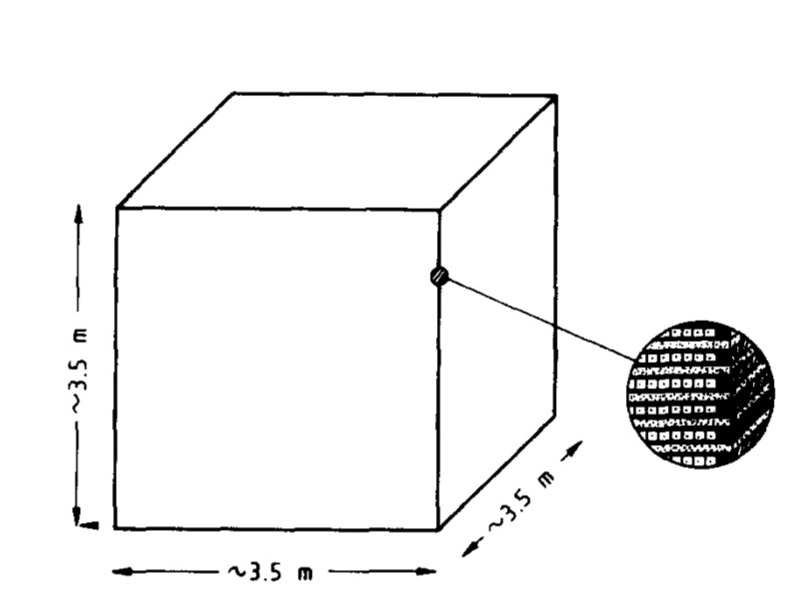
\includegraphics[width=0.49\textwidth]{figures/nusex1.jpeg}
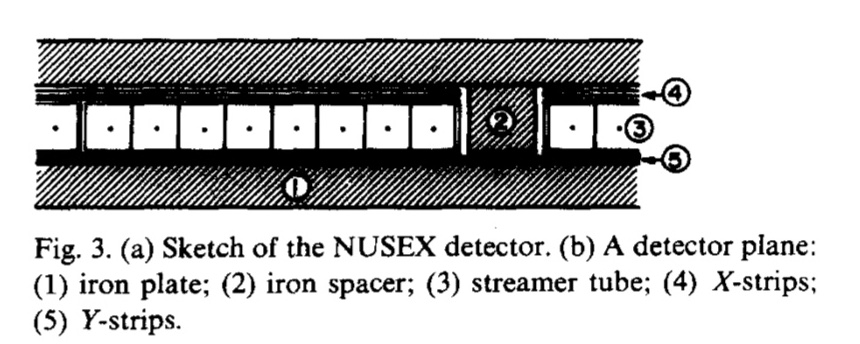
\includegraphics[width=0.49\textwidth]{figures/nusex2.jpeg}
\vspace{2mm}
\caption{A sketch of the NUSEX detector with various parts highlighted~\cite{56NUSEX}.}
\label{fig:nusex}
\end{figure}

\begin{figure}[h!]
\centering
  \centering
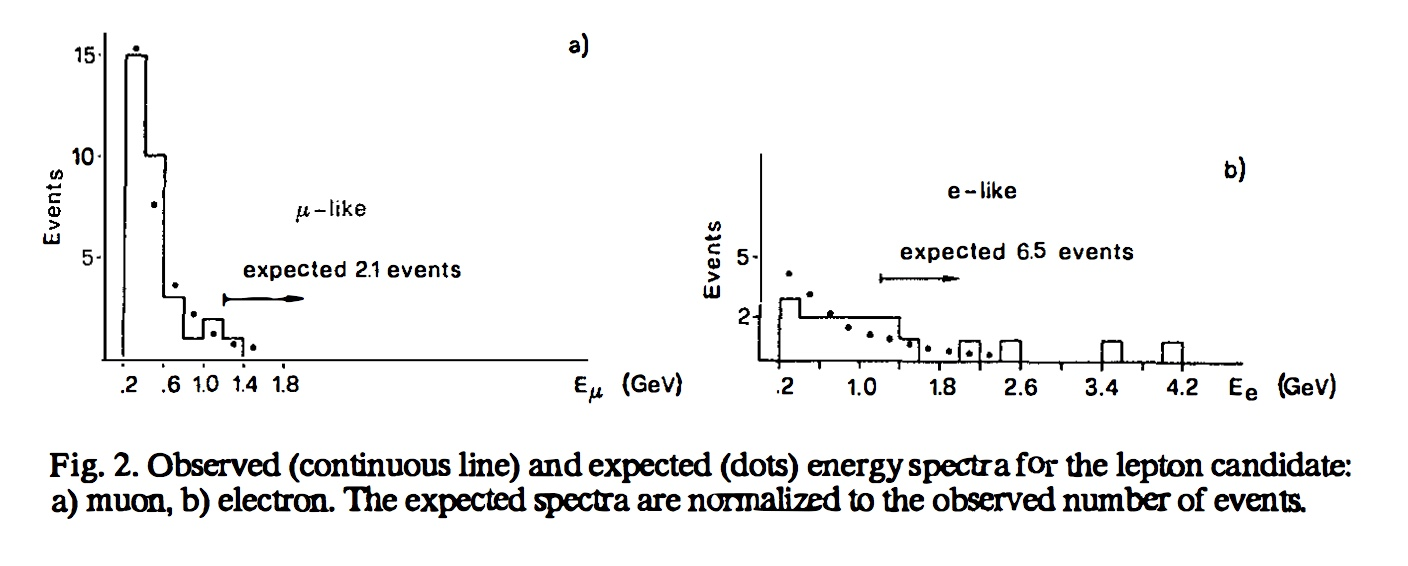
\includegraphics[width=0.5\textwidth]{figures/nusexres.jpeg}
\vspace{2mm}
\caption{Data compared to Monte Carlo for 50 neutrino events in the NUSEX and showing consistency within errors~\cite{57NUSEX}.}
\label{fig:nusexres}
\end{figure}

\subsection{KamiokaNDE}
The Kamioka Nucleon Decay Experiment (KamiokaNDE) is a 3000 ton water Cherenkov detector installed in the Kamioka mine 1000 m under the top of a mountain. The detector has the aim to study and search for nucleon decay which began operation in 1983. The Cherenkov light is detected using 1000 large PhotoMultiplier Tubes (PMTs)~\cite{58KAMIOKA}.


\if{0}
 In Japan, the Kamiokande detector (1983-1996, 3 kiloton) and Super-Kamiokande (in operation since 1996, 50 kiloton) have achieved several important scientific results, notably detection of extraterrestrial neutrinos from the Sun [40] and Supernova 1987a [41, 42], and discovery of neutrino flavor mixing and neutrino mass [6, 43]. In the K2K long baseline neutrino oscillation experiment, Super-K and a one kiloton water Cherenkov detector (1KT) provided indis- pensable data on the neutrino beam flux and its energy spectrum at the neutrino production site (using 1KT) and a location 250 km farther away (using Super-K) [22]. Super-K again is playing the role of the far detector in the ongoing T2K experiment which reported an indication of %νμ → νe oscillations in June 2011 [1].
Good paper for all of this! %https://arxiv.org/pdf/1109.3262.pdf
6, Y. Fukuda et al. (Super-Kamiokande), Phys. Rev. Lett. 81, 1562 (1998), arXiv:hep-ex/9807003.
40, K. S. Hirata et al. (KAMIOKANDE-II), Phys. Rev. Lett. 63, 16 (1989).
41, K. Hirata et al. (KAMIOKANDE-II), Phys. Rev. Lett. 58, 1490 (1987).
42, K. S. Hirata et al. (KAMIOKANDE-II), Phys. Rev. D38, 448 (1988).
43, S. Fukuda et al. (Super-Kamiokande), Phys. Lett. B539, 179 (2002), arXiv:hep-ex/0205075
Kamiokande2 was solar?
\fi
\begin{figure}[h!]
\centering
  \centering
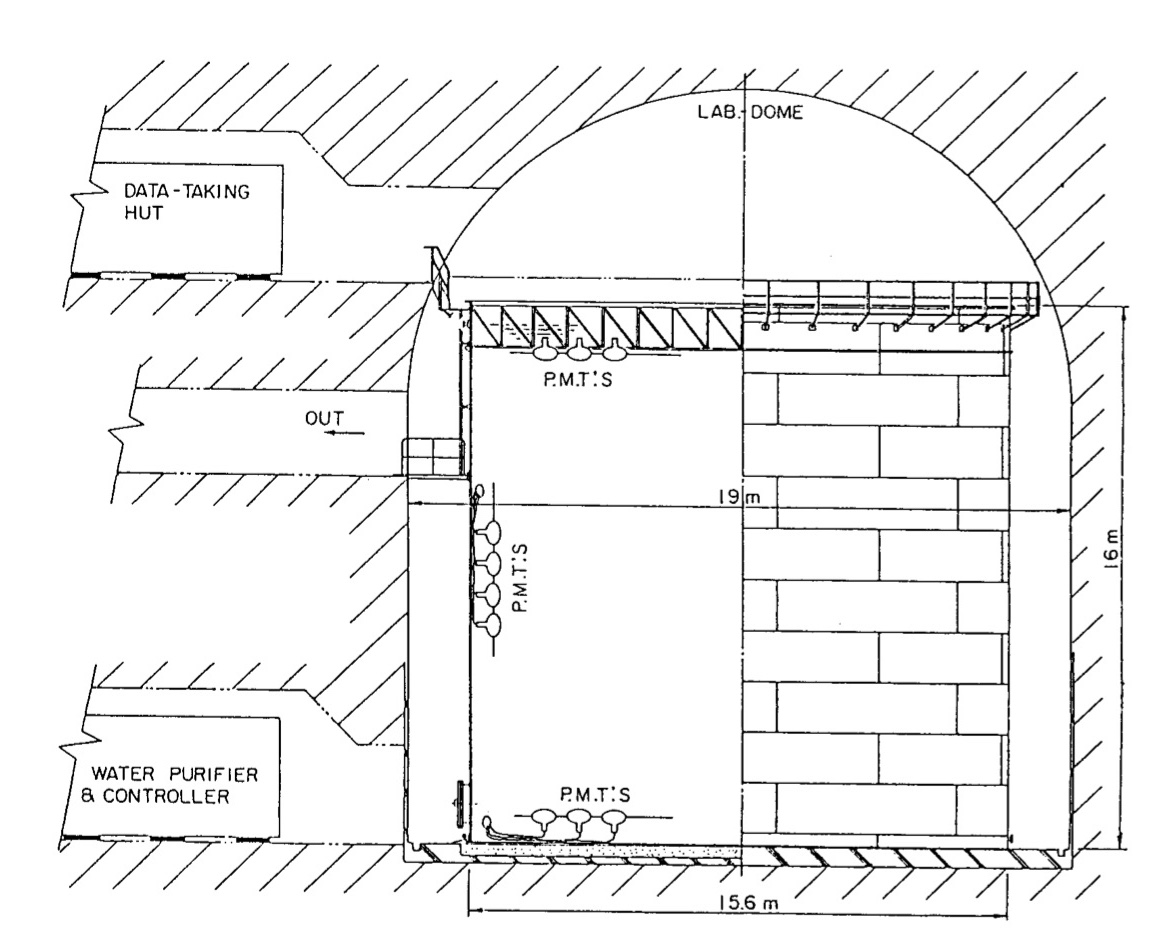
\includegraphics[width=0.5\textwidth]{figures/Kamioka1.jpeg}
\vspace{2mm}
\caption{Schematic image of the KamiokaNDE detector.~\cite{58KAMIOKA}.}
\label{fig:Kam}
\end{figure}

\begin{figure}[h!]
\centering
  \centering
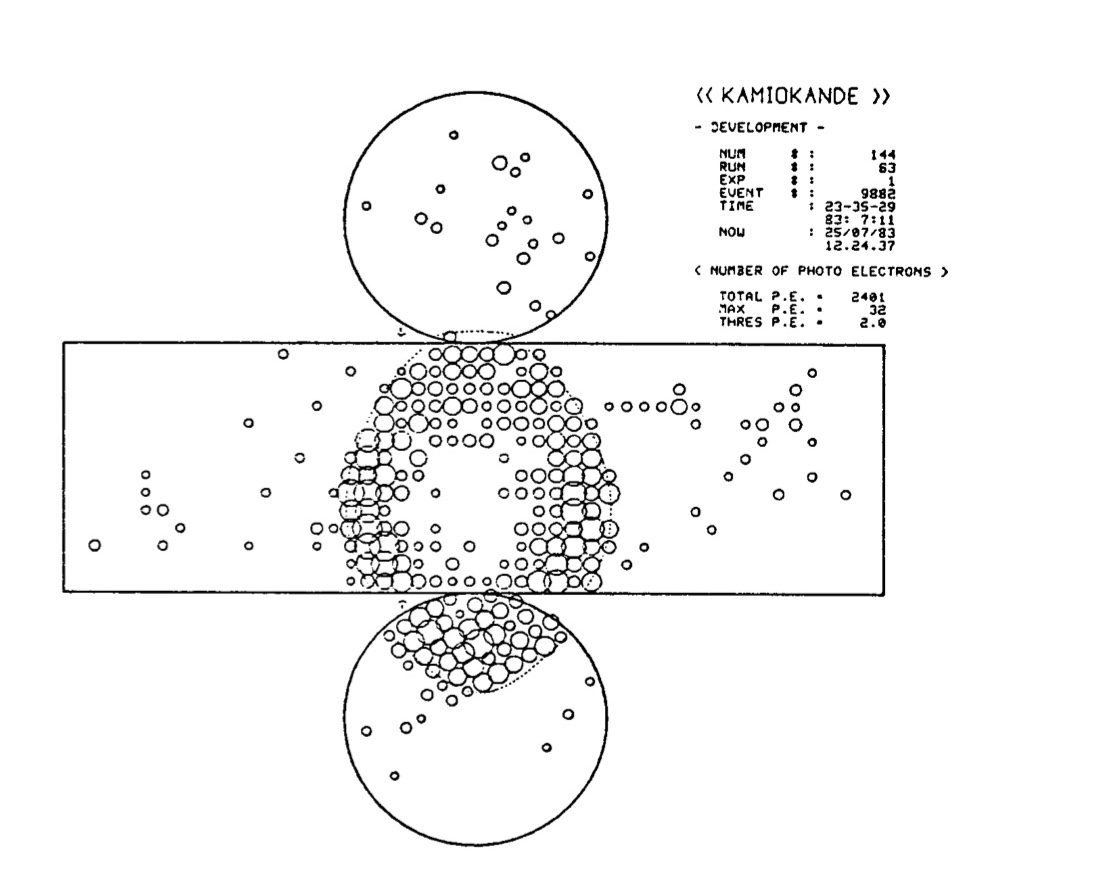
\includegraphics[width=0.49\textwidth]{figures/Kamioka2.jpeg}
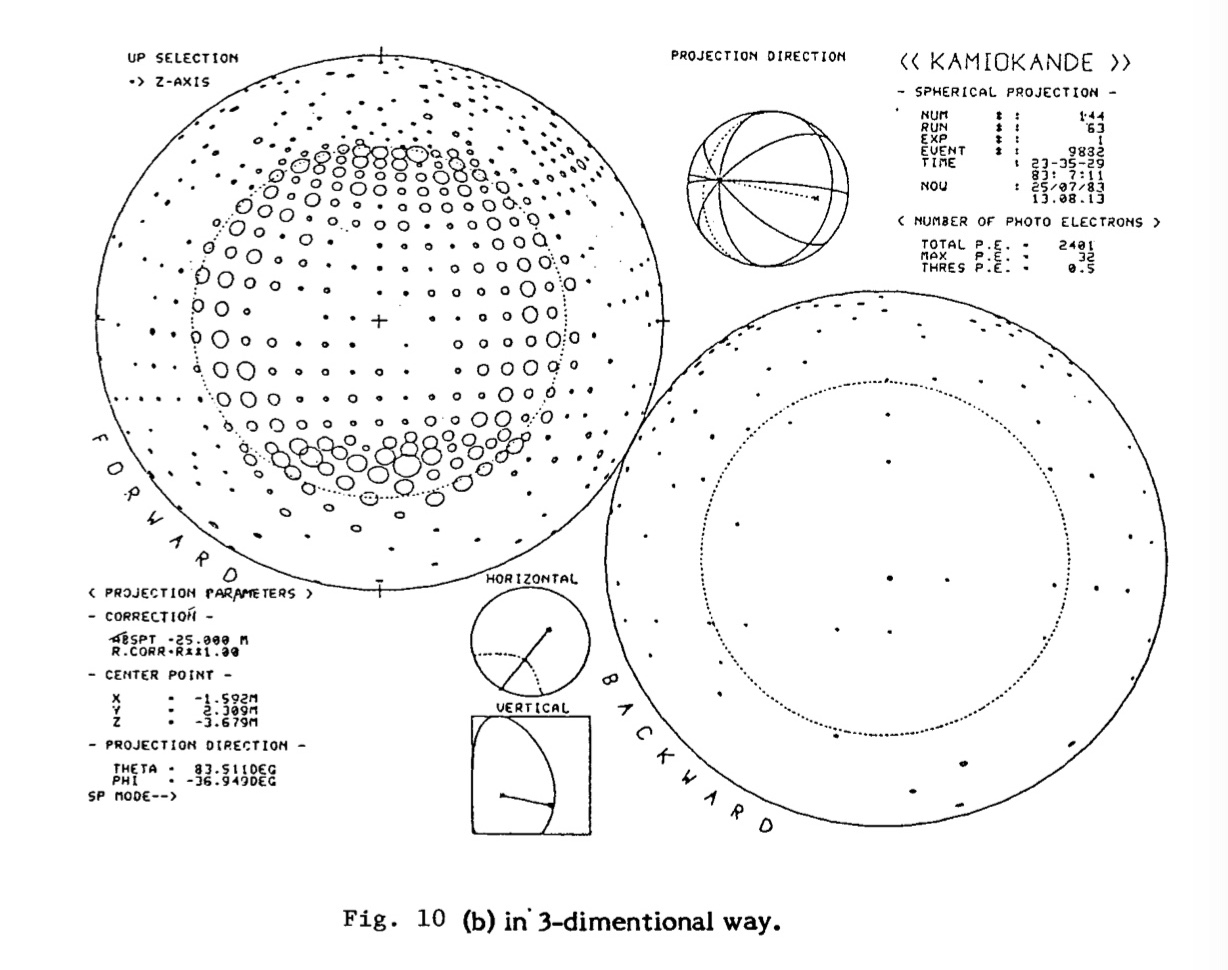
\includegraphics[width=0.49\textwidth]{figures/Kamioka3.jpeg}
\vspace{2mm}
\caption{A sample event showing Cherenkov rings produced by a muon event~\cite{58KAMIOKA}.}
\label{fig:Kam2}
\end{figure}
The main result was finding a slight discrepancy between data and simulations, seen in \FigRef{fig:Kam3}, hinting at at a possibility that atmospheric neutrinos were oscillating.
\begin{figure}[h!]
\centering
  \centering
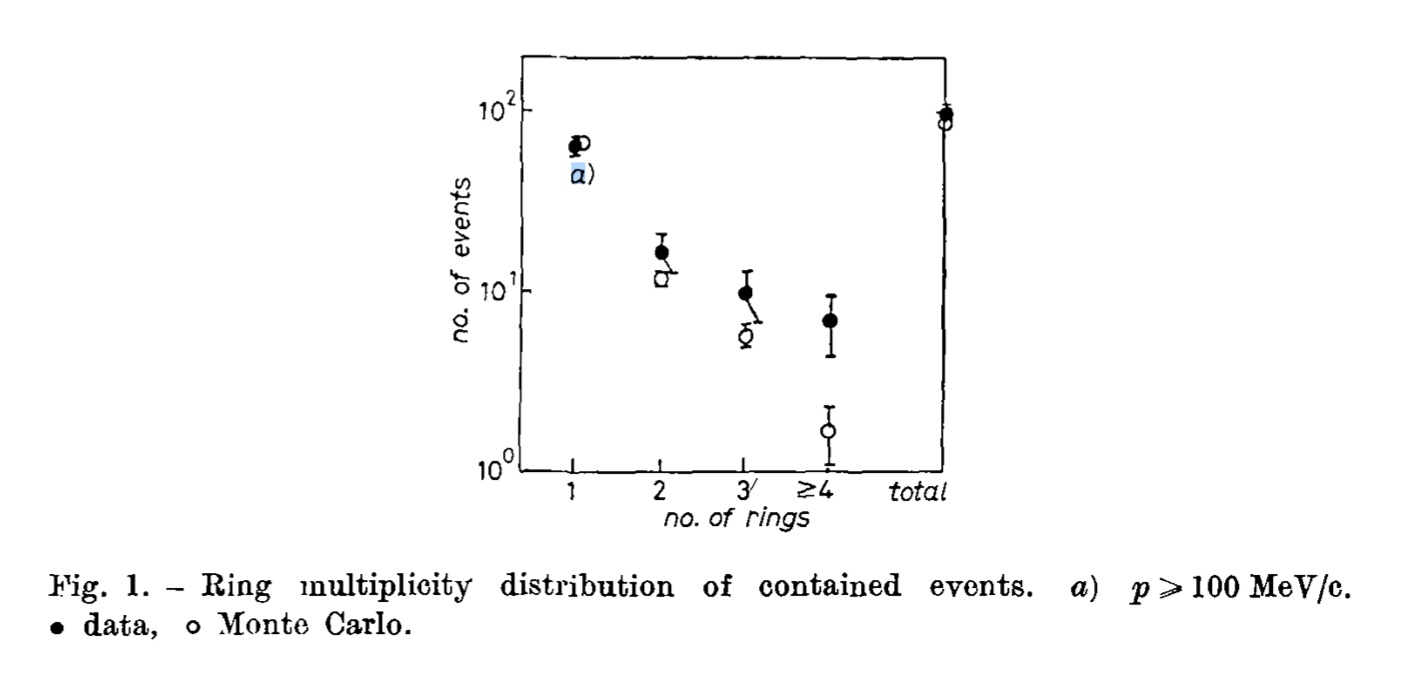
\includegraphics[width=0.49\textwidth]{figures/Kamioka4.jpeg}
\vspace{2mm}
\caption{Comparing ring multiplicity distributions between data and simulations~\cite{59KAMIOKA}.}
\label{fig:Kam3}
\end{figure}

\subsection{IMB}
The Irvine- Michigan-Brookhaven (IMB) groups build a 8 kiloton water Cherenkov detector 600 m under the Morton Salt Mine in Cleveland which began data taking in 1986. The design was similar to KamiokaNDE and managed to improve several results including improving the parameter space of neutrino oscillation~\cite{60IMB}.


\subsection{Super-Kamiokande}
Super-Kamiokande\cite{20SUPERK}, a water Cherenkov detector is located 1 km underground and consists of a cylindrical stainless steel tank holding 50 ktons of ultra-pure water, performed the first experimental observation that the neutrino has non-zero mass\cite{10Fukuda} and also managed to detect strong evidence of muon neutrino oscillation to tau neutrinos from the analysis of atmospheric neutrinos interacting in the water target~\FigRef{fig:SK2}. The deviation from 1 shows the discovery of neutrino oscillations and the lines show the expected shape for oscillation from muon neutrinos to tau neutrinos~\cite{10Fukuda}. It also shows that electron-like events have no significant variation in length over neutrino energy where at large length over neutrino energy muon-like events have come to close to half of the initial rate.

\begin{figure}[h!]
\centering
  \centering
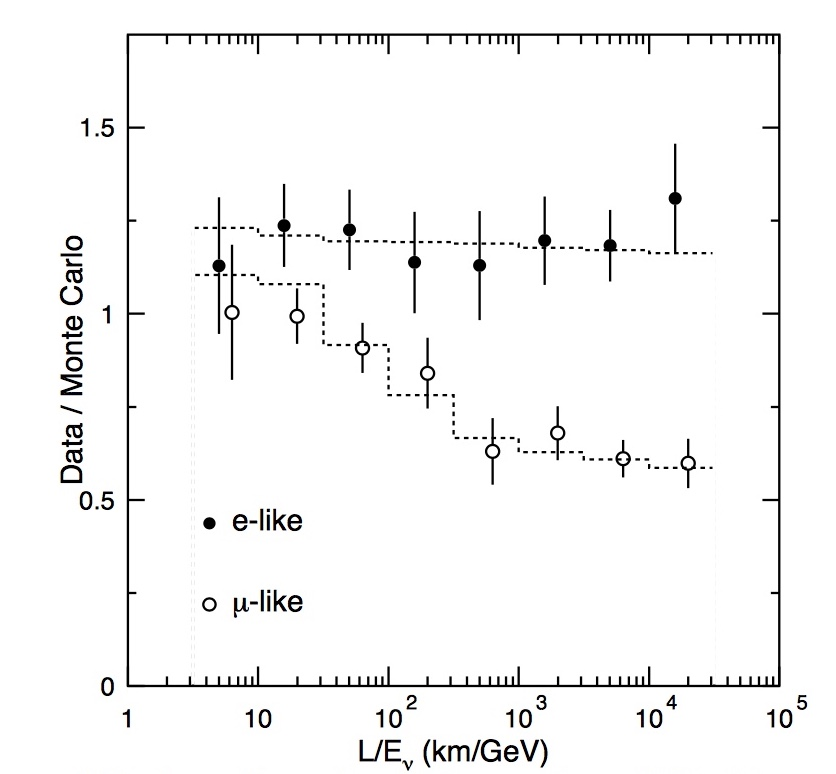
\includegraphics[width=0.49\textwidth]{figures/simuSK2.jpeg}
\vspace{2mm}
\caption{Comparison of the ration of data vs Monte Carlo vs length over neutrino energy for fully contained atmospheric electron-like and muon-like events~\cite{10Fukuda}.}
\label{fig:SK2}
\end{figure}

\begin{figure}[h!]
\centering
\begin{subfigure}{.5\textwidth}
  \centering
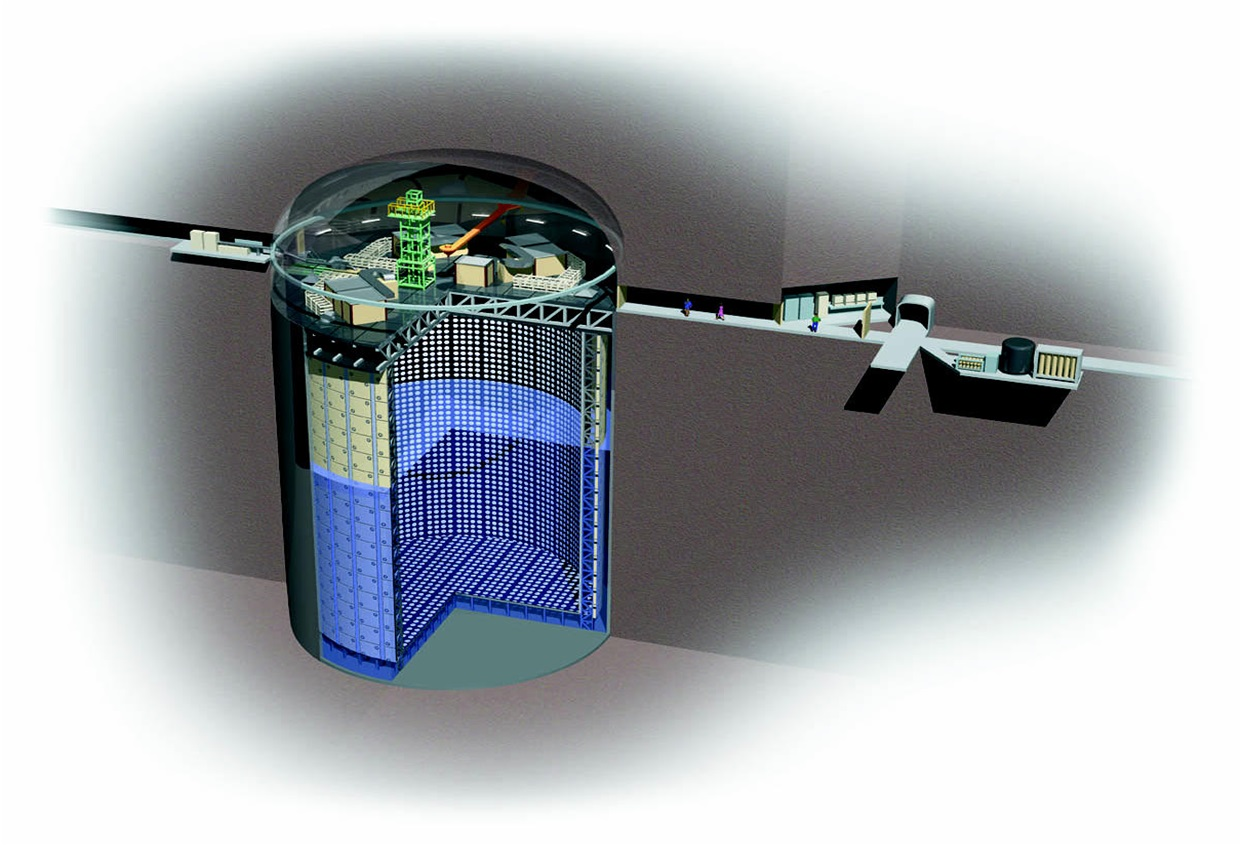
\includegraphics[width=\textwidth]{figures/SK3D.jpg}
\vspace{2mm}
  %\label{fig:sub1}
\end{subfigure}%
\begin{subfigure}{.5\textwidth}
  \centering
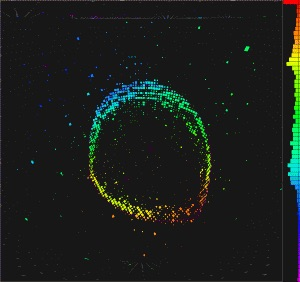
\includegraphics[width=0.7\textwidth]{figures/SuperKMuon-300x282.jpg}
\vspace{2mm}
  %\label{fig:sub2}
\end{subfigure}
\vspace{2mm}
\caption{Left) A schematic of the Super-K detector., Right) Event recorded in Super-K.}
\label{fig:SK}
\end{figure}
% http://t2k-experiment.org

\subsection{MACRO}
The Monopole, Astrophysics and Cosmic Ray Observatory (MACRO) was combined of liquid scintillation counters, limited streamer tubes and nuclear track detectors allowing it to searching for signs of magnetic monopoles, as well as being able to operate as a neutrino detector as well as search for other phenomena. Data was taken between 1995 until 2000 and by measuring neutrin induced muons, the MACRO managed to aid in the discovery of atmospheric neutrino oscillation~\cite{62MACRO}

\begin{figure}[h!]
\centering
  \centering
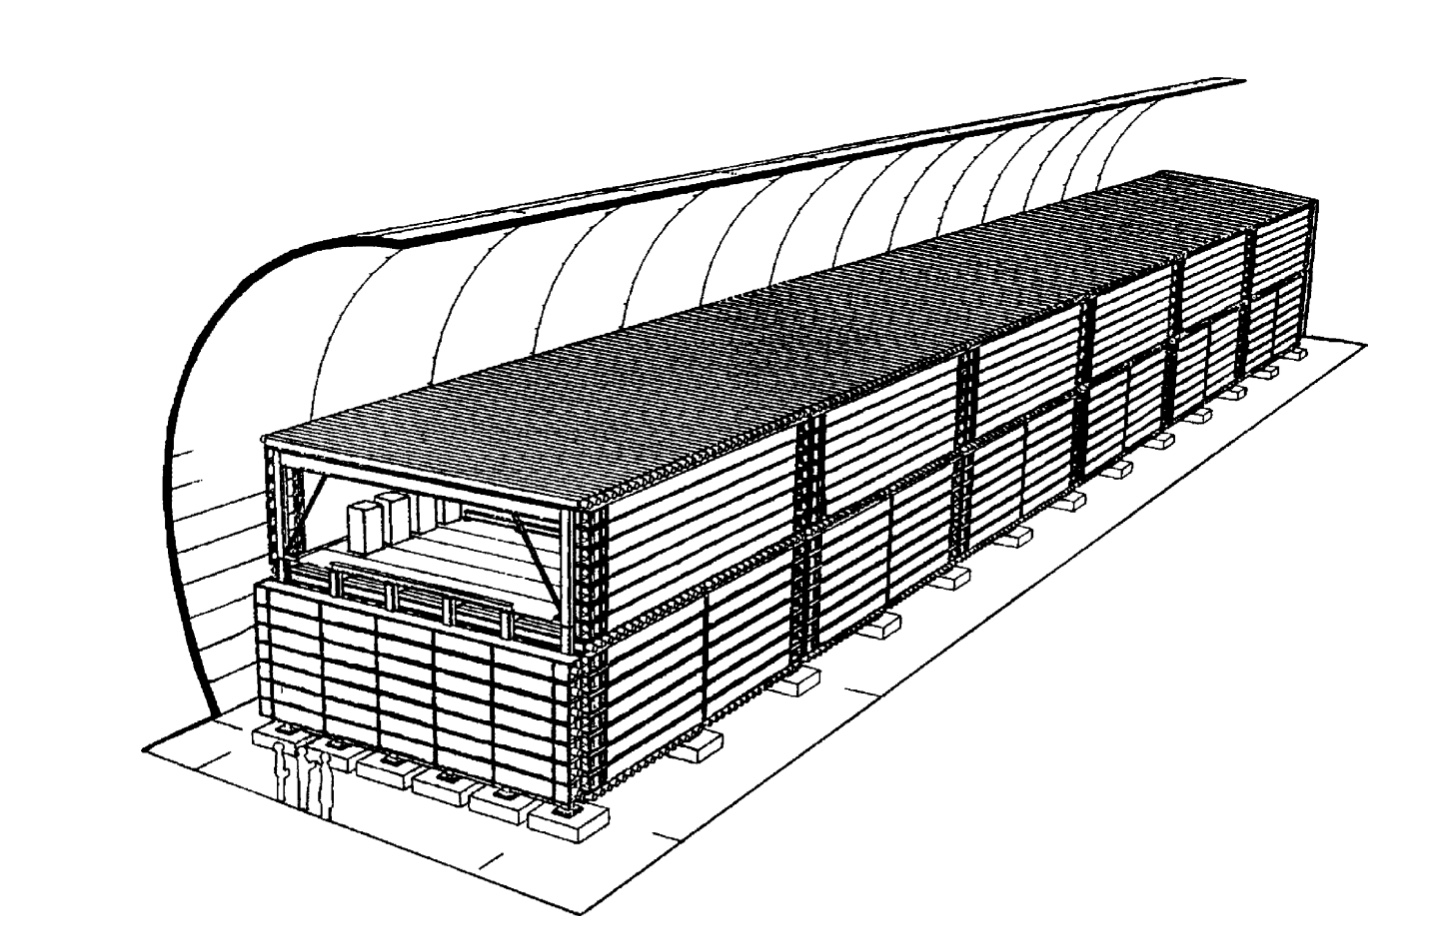
\includegraphics[width=0.49\textwidth]{figures/MACRO.jpeg}
\vspace{2mm}
\caption{Schematic of the MACRO~\cite{61MACRO}.}
\label{fig:Kam3}
\end{figure}

\section{Solar}
The mechanism for neutrino generation in the sun was briefly discussed in subsection~\ref{subsection:Missing}.
Solar neutrinos are interested for both allowing a unique way of probing the internal solar reactions as well as providing a very baseline combined with energies of around $1 MeV/c$ allowing probing of mass differences in the range of $\Delta m^2 \approx 1-^{-10} eV^2$ through neutrino oscillation, see equation~\ref{eq:twoPNeutrinoosc}. Based on current experimental values these experiments are sensitive for $\theta_{12}$ and $\Delta m_{12}^2 $

Mention best values and different hierarchy?

\subsection{Super-Kamiokande}

Super-Kamiokande, as described above, could thanks to its design also be used for solar neutrino studies and extended the neutrino oscillation analysis to lower mass difference values as well as performed solar interaction measurements~\cite{64SuperK}.

\subsection{SNO}
The Sudbury Neutrino Observatory (SNO)~\cite{Fix6} was build to make a definite measurement of solar neutrinos following the measurements taken by the Homestake experiment~\cite{9Davis}. It utilized PMT (Photo Multiplier Tubes) to measure Cherenkov radiation produced by neutrino interactions in the detectors 1000 ton ultra-pure heavy water volume. The whole detector is placed 2 km underground to minimize background interactions. It expanded on looking for a specific energy range for cosmic rays, Boron decay, to becoming a generic neutrino detector meaning that other atmospheric and cosmic neutrinos became background events for measuring solar neutrinos. The experiment has a unique ability to separate the reactions between electron neutrino charge current (CC), neutral current interactions (NC) with all flavours of neutrinos and with electron scattering (ES). With this observed neutrino flux observed through CC reactions could be compared to that of the ES  and NC to provide evidence for a neutrino flavour change regardless of the predictions of solar modes.

The experiment clearly showed a significant difference in flux between CC interactions, only available with electron neutrinos compared to expected and compared to the NC and ES interactions. The result can be seen in \FigRef{SNO2}.

\begin{figure}[h!]
\centering
\begin{subfigure}{.5\textwidth}
  \centering
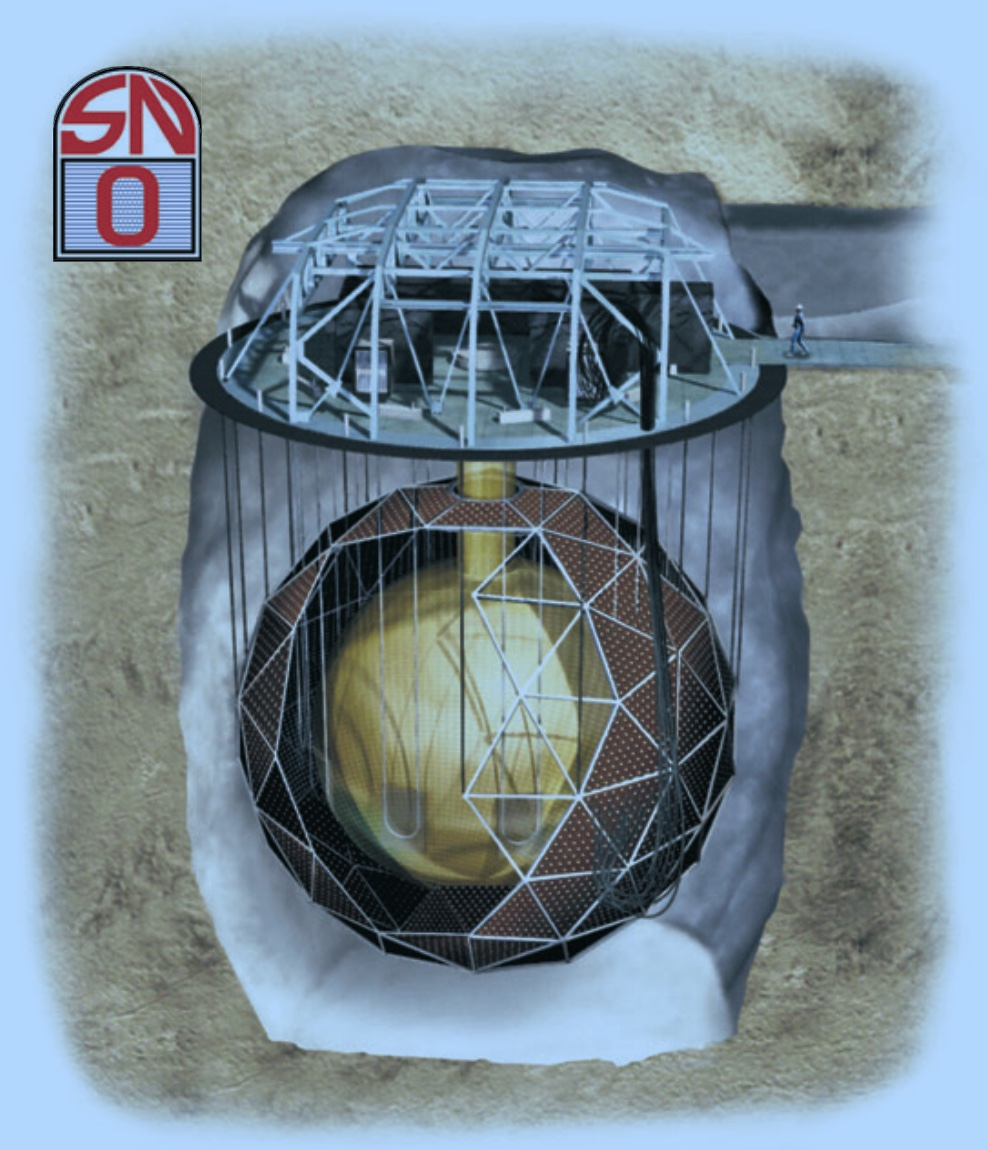
\includegraphics[width=0.7\textwidth]{figures/sno.jpeg}
\vspace{2mm}
  %\label{fig:sub1}
\end{subfigure}%
\begin{subfigure}{.5\textwidth}
  \centering
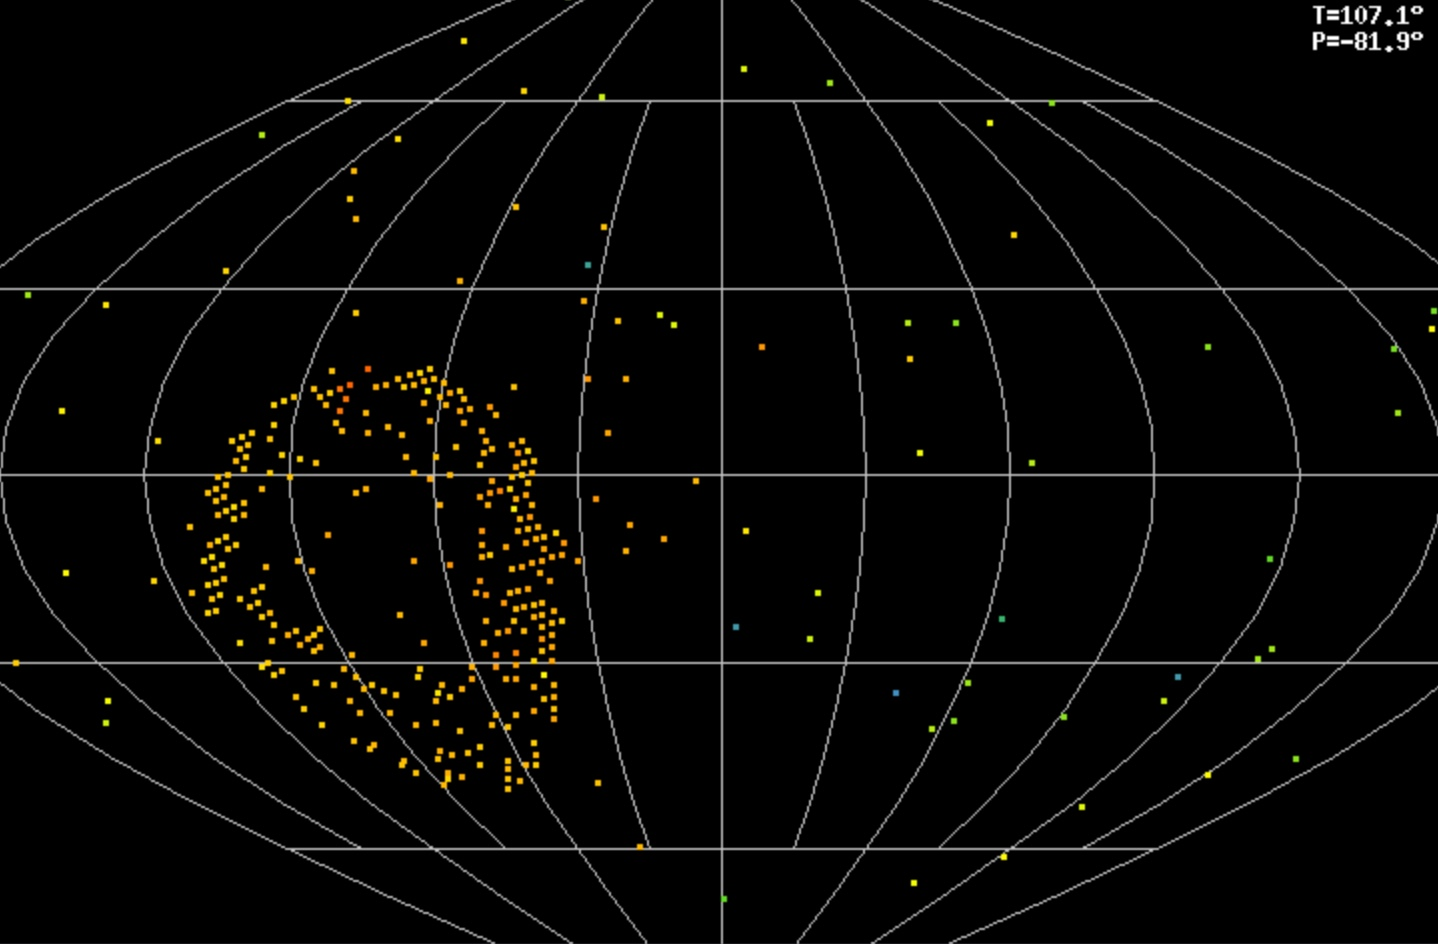
\includegraphics[width=\textwidth]{figures/SNOmuonEvent.jpeg}
\vspace{2mm}
  %\label{fig:sub2}
\end{subfigure}
\vspace{2mm}
\caption{Left) A schematic drawing of the SNO detector~\cite{Fix6}, Right) Cherenkov light recorded from a muon created by interaction of an atmospheric neutrino in the heavy water.}
\label{fig:SNO}
\end{figure}

\begin{figure}[h!]
\centering
  \centering
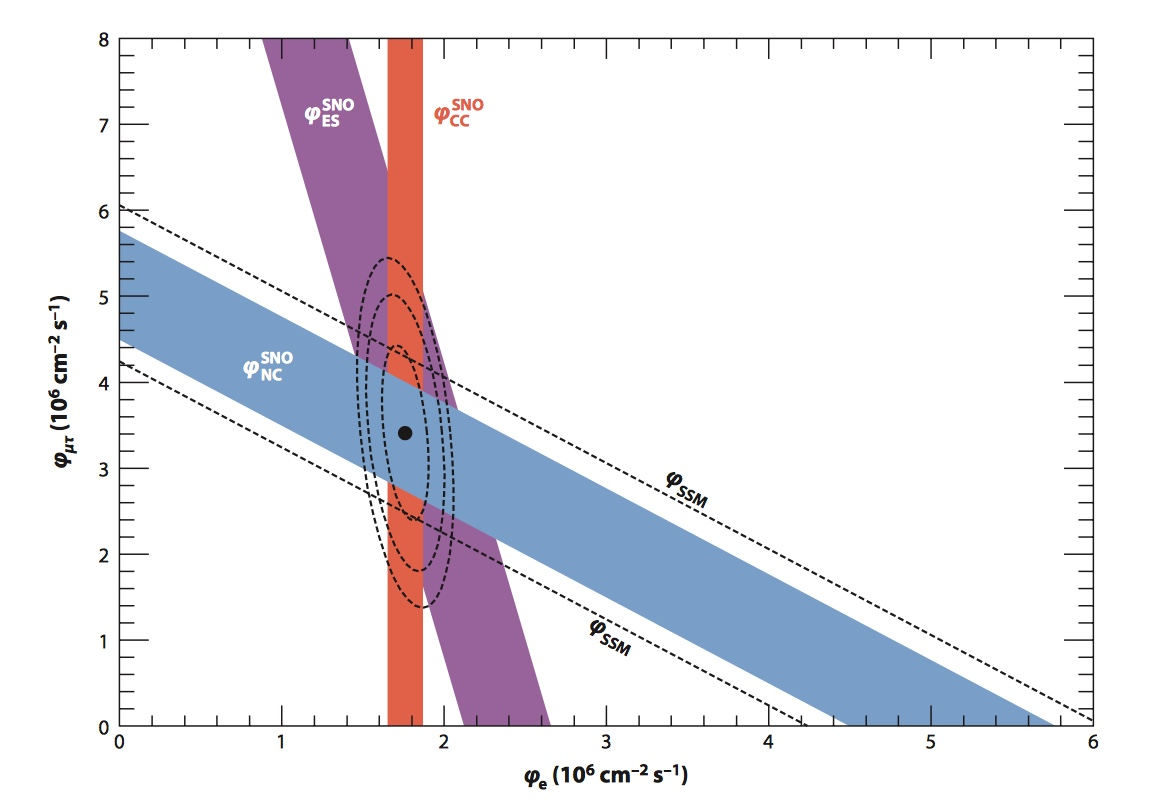
\includegraphics[width=0.49\textwidth]{figures/snoSpec.jpeg}
\vspace{2mm}
\caption{The flux of solar neutrinos of $\mu$ or $\tau$ flavour vs flux of electron neutrinos measured in SNO from the three reactions, CC in red, ES in purple and NC in blue.The diagonal dashed lines show the prediction from the Standard Solar Model. The coloured bands intersect at the fit values for all fluxes indicating that they are consisted with neutrino flavour transformation with no distortion in the solar neutrino energy spectrum. ~\cite{Fix6}.}
\label{fig:SNO2}
\end{figure}

The experiment is currently replacing the heavy water with liquid scintilator and renaming itself as SNO+~\cite{42SNO+}.

\subsection{Borexino}
Started data taking in May 2007. Ongoing. measure solar neutrinos very precise measurements of neutrino fluxes from sun.limits on charge non conservation. limits on sterile neutrinos and geoneutrinos. pep solar neutrinos first measurement.

Borexino is a liquid scintillator detector making it more sensitive, especially to the low energetic solar neutrinos, than Cherenkov techniques but lacks the ability to detect directionality of incoming particles requiring an extremely low radioactive contamination of the scintillator media. This is handled by containing the detector within shielding material and utilizing ultra pure materials~\cite{63Borexino}. The scintillating light is then read out by PMTs uniformly distributed around the active volume seen in \FigRef{fig:borexino}.

\begin{figure}[h!]
\centering
  \centering
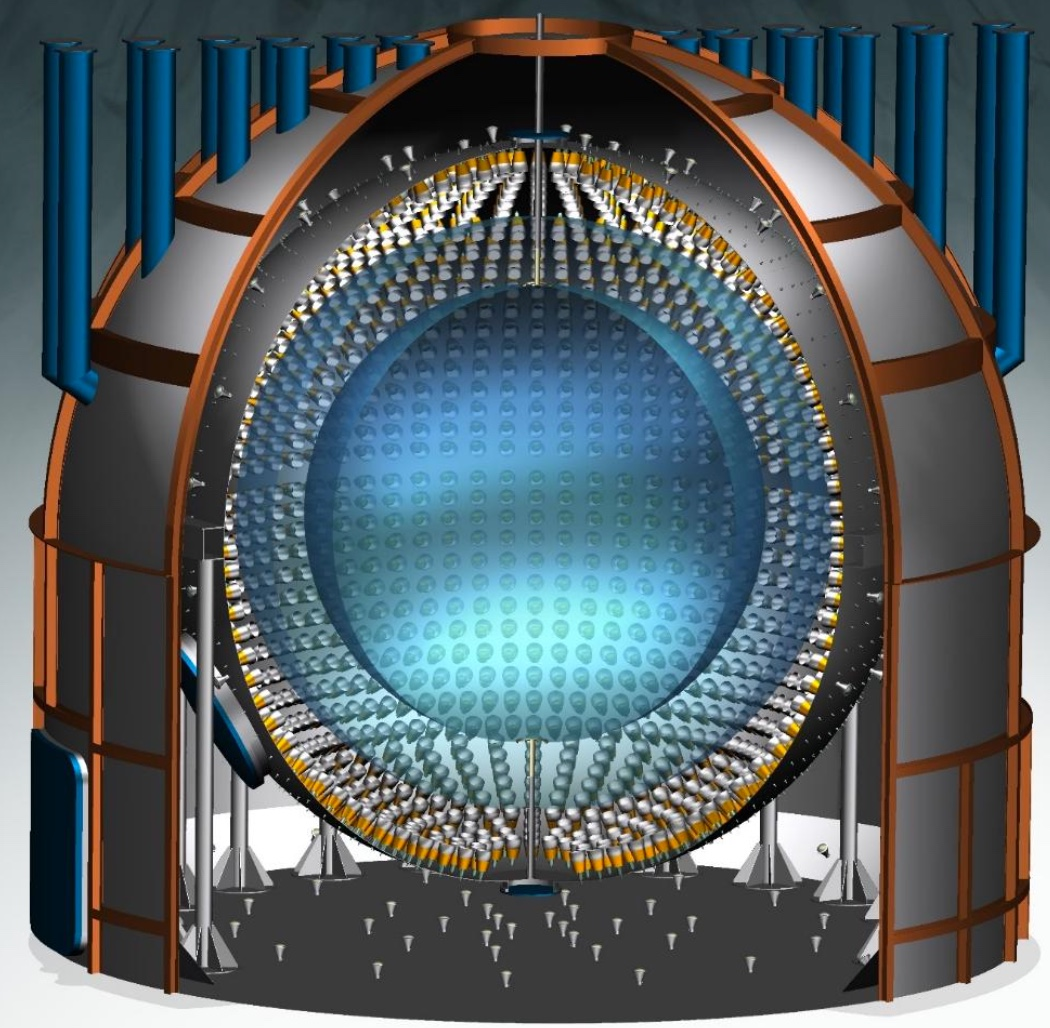
\includegraphics[width=0.49\textwidth]{figures/borexino.jpeg}
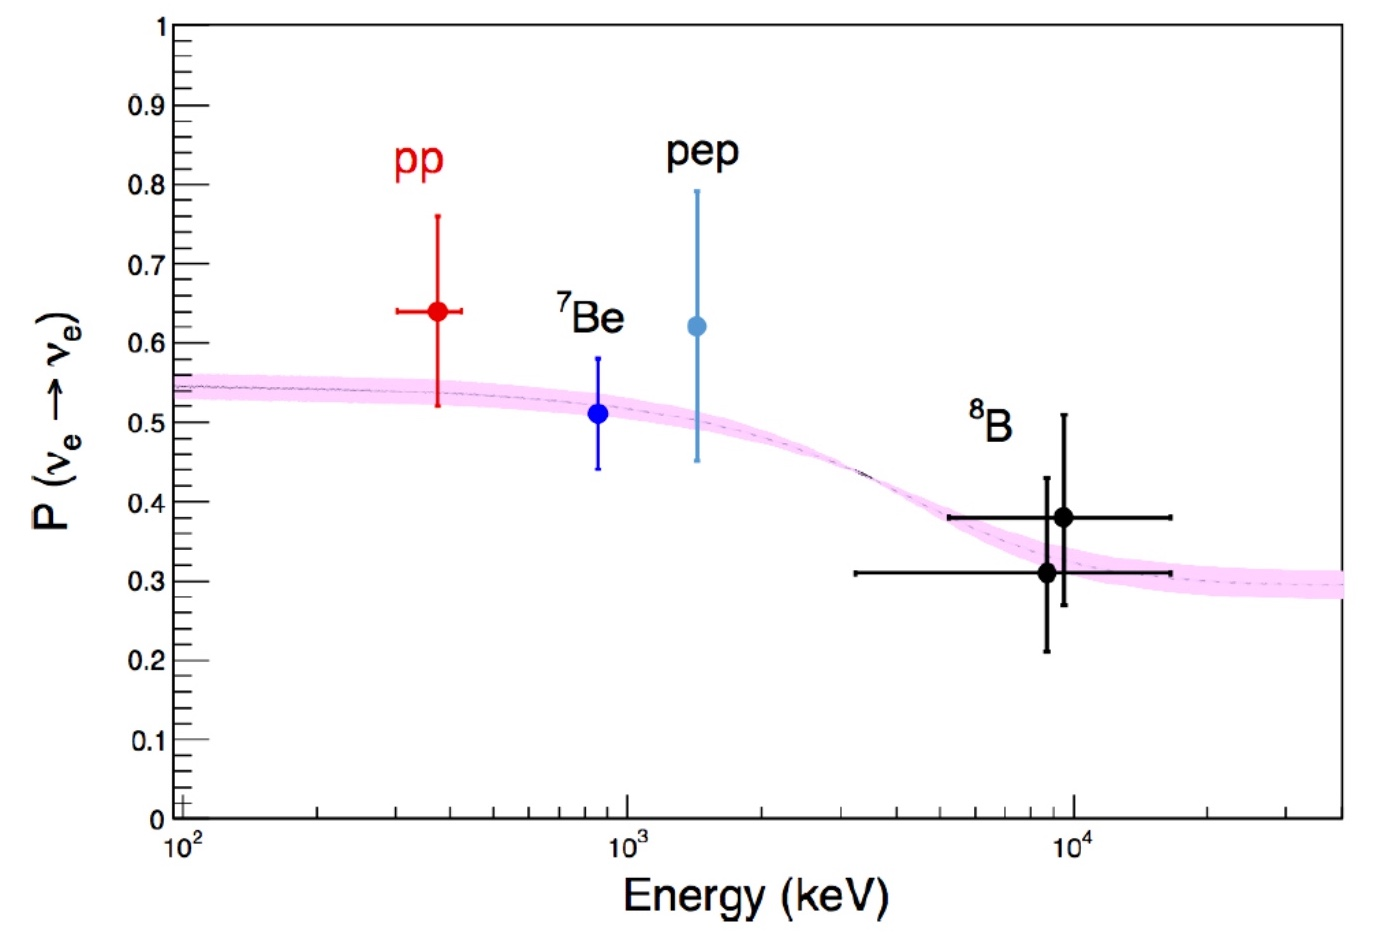
\includegraphics[width=0.49\textwidth]{figures/borexino3.jpeg}
\vspace{2mm}
\caption{(Left) Schematic of the Borexino experiment~\cite{63Borexino}. (Right) Electron neutrino survival probability as a function of neutrino energy according representing different neutrino solar production channels both from the Solar standard model and measurements from the Borexino experiment~\cite{63Borexino}.}
\label{fig:borexino}
\end{figure}

quote!

5. Conclusion
\textbf{The most recent solar and terrestrial neutrino results stemmed from Borexino have further reinforced the ultra-low background achievements of this experiment, an exceptional breakthrough in the field of techniques for rare processes search. The 7Be, 8B, pep and the very recently measured pp components have all been detected (together with a tight upper limit on CNO), leading to the validation of the MSW-LMA oscillation paradigm in the entire energy regime of the solar neutrinos, strengthened also by the determination of the absence of day-night asymmetry in the 7Be flux. Very remarkably, Borexino performed this validation with its own data, without the need to resort to the results of other solar neutrino experiments.
Finally, the highly significant measurement of the terrestrial neutrinos not only complements the physics potentiality of the detector, but points towards a future new direction of research in the studies of the interior of the Earth.}

\section{Accelerator}
Currently accelerator facilities can produce muon and electron neutrinos and anti neutrinos from accelerated protons. Protons are accelerated in a particle accelerator where the energy of the protons is related to the energy of the neutrinos. The proton beam is then directed at a target where the protons interact with the target material, producing a large number of secondary pions (among other particles). Shaped magnetic fields, so called focusing horns, are used to select out pions of the preferred charge (positive for a neutrino beam, negative for an antineutrino beam) in a specific momentum range and focus them into a collimated beam. The beam is directed into a long decay volume, where the pions decay into muons and (anti)neutrinos. At the end of the decay volume there is a large mass of material which absorbs all the particles except the neutrinos. This provides a nearly pure beam of muon-neutrinos (or muon-antineutrinos if negatively charged pions are selected). There is some inevitable contamination from antineutrinos in the neutrino beam or neutrinos in the antineutrinos beam and from electron-neutrinos, mostly because the original pion beam also includes some kaons, which can decay to produce electron-neutrinos as well as from muon interactions. To differentiate between these accelerator-based neutrino experiments, like reactor experiments, generally use a near detector as well as a far detector. This configuration allows comparison of the neutrino beam at the near detector with the far detector to determine if there has been any neutrino oscillation.

The advantage of accelerator neutrinos are that the energy range is well known and can be quite well tailored, the flux is huge compared to other methods. However the energy distribution will be quite wide because of the decay processes involved. It is also hard to produce a clean beam without background, muon neutrinos without electron neutrinos. However, for oscillation experiments this can be a good thing, see subsection \ref{subsec:nuFACT}. Based on current experimental values these experiments are sensitive for $\theta_{23}$ and $\Delta m_{23}^2 $

\subsection{Historical experiments}
%The European Organization for Nuclear Research, (CERN) has had accelerator neutrino experiments and some based around magnetised volumes to provide change identification of particles. 

The European Organization for Nuclear Research (CERN) Dortmund Heilelberg Saclay Warsaw (CDHSW)~\cite{40CDHSW} experiment was designed to study neutrino interactions in iron using the CERN SPS neutrino beam line. The experiment consisted of two similar detectors at different distances from the interaction vertex 130 m and 885 m~\cite{40CDHSW}.The detectors were built designed to combine the functions of a muon spectrometer and a hadron calorimeter. It consisted of 19 toroidal magnetised iron modules, with an average field of 1.65 T, separated from each other by wire drift chambers and had a mass of 1250 tons. In the end of the experiment a liquid hydrogen tank was placed in front of the experiment to study neutrino interactions in hydrogen. This is one of the first MINDs (Magnetised Iron Neutrino Detectors).

The CHARM Collaboration (CERN-Hamburg-Amsterdam-Rome-Moscow Collaboration) proposed to study neutrino-nucleon neutral current interaction as well as muon polarisation. It took data from 1978 to 1991 and  was comprised of a fine-grained target calorimeter made up of 78 subunits each surrounded by a frame of magnetized iron for muon identification and spectrometry~\cite{68CHARM}.

The CCFR (University of Chicago, Columbia University, Fermilab, and the University of Rochester) detector installed at Fermilab consists of an 18 m long 690 ton neutrino target calorimeter and followed by an iron toroid spectrometer. The calorimeter consists of 168 iron plates, each 3m x 3m x 5.1cm, with liquid scintillation counters spaced between every two plates and drift chambers spaced every four plates. It provided among other things, precision measurements fro neutrino-nucleon scattering~\cite{67CCFR}. The experiment was continued through the NuTeV experiment which expanded results using the same detector. CCFR took data from 1979 to 1988, NuTeV started in 1996 and continued until 2003.

\subsection{NOMAD}
The Neutrino Oscillation Magnetic Detector (NOMAD)~\cite{NOMADexp}, also using the CERN SPS neutrino beam line, searched for $\nu_\mu \rightarrow \nu_\tau$ oscillation by detecting $\tau$ appearance. Its goals were to measure the momenta of charged particles and identify and measure electron, photons and muons. By the detector design it was also possible to look for $\nu_\mu \rightarrow \nu_e$ oscillation. Compared to the modular design of CDHS, NOMAD had drift chambers and other subdetectors contained inside a dipole magnet at 0.4 T.

%\textbf{RESULTS?}
\begin{figure}[h!]
\centering
  \centering
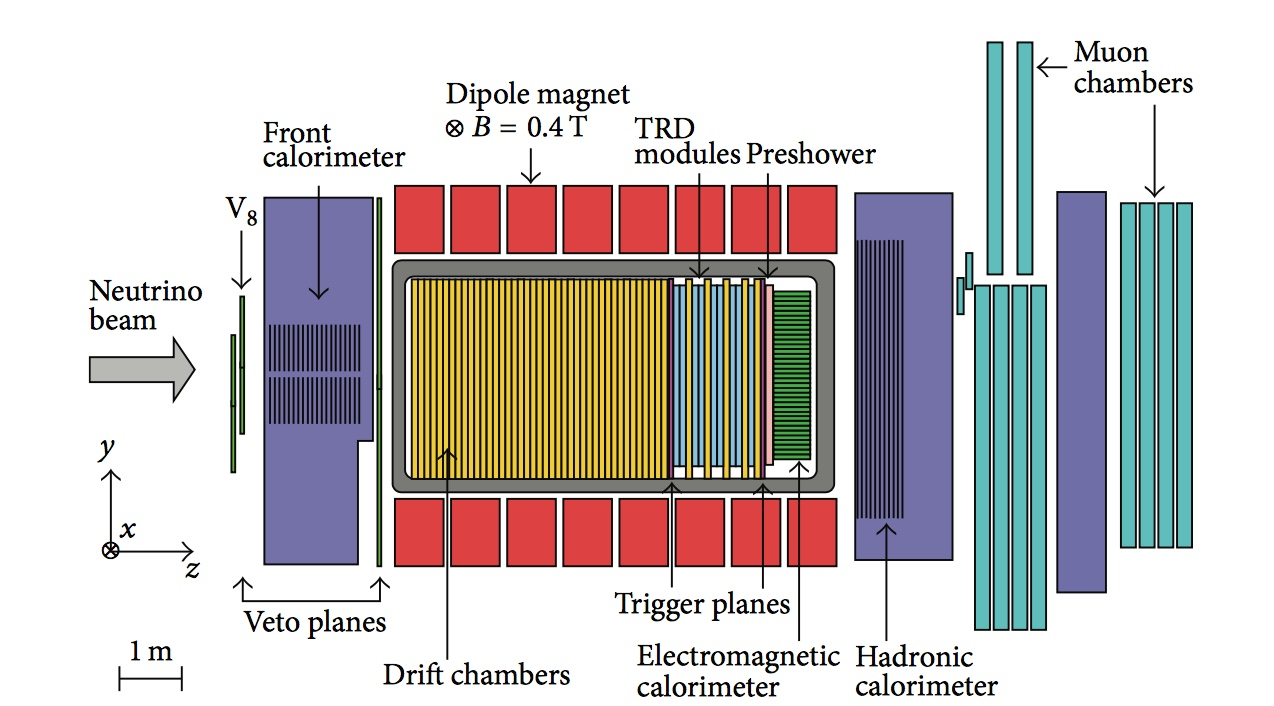
\includegraphics[width=0.7\textwidth]{figures/NOMAD2.jpeg}
\vspace{2mm}
\caption{A sideview of the NOMAD detector~\cite{69NOMAD}.}
\label{fig:NOMAD}
\end{figure}

\subsection{K2K}
After the success of Super-Kamiokande, the KEK to Kamiokande (K2K) experiment\cite{22K2K} was created with the main difference of using a well understood muon neutrino beam pointing at the Super-Kamiokande detector at a distance of 250 km. It was the first neutrino oscillation measurement where both the source and detector were controlled, it observed the disappearance of muon neutrinos into tau neutrinos and found results that were consistent with Super-Kamiokande.

K2K, the set up seen in~\FigRef{fig:K2K} and ran from 1999 to 2004, used a neutrino beam with a wide spectrum peaked at 1 GeV based on a 12 GeV proton synchrotron beam which interacts with an aluminium target and focused through two horns and allowed to decay in a 200 m long decay pipe. This creates a 98\% pure muon neutrino beam with around 1\% contamination of anti muon neutrinos and around 1\% electron and anti-electron neutrinos. Understanding the beam is required for looking at $\nu_\mu \rightarrow \nu_e$ appearance requires a good understanding of the beam composition. To do this a 1-kiloton water Cherenkov near detector,  a scaled-down version of Super-Kamiokande, is used to measure the neutrino spectrum which is then extrapolated using Monte Carlos simulated data to provide a neutrino spectrum at Super-Kamiokande detector.

\begin{figure}[h!]
\centering
  \centering
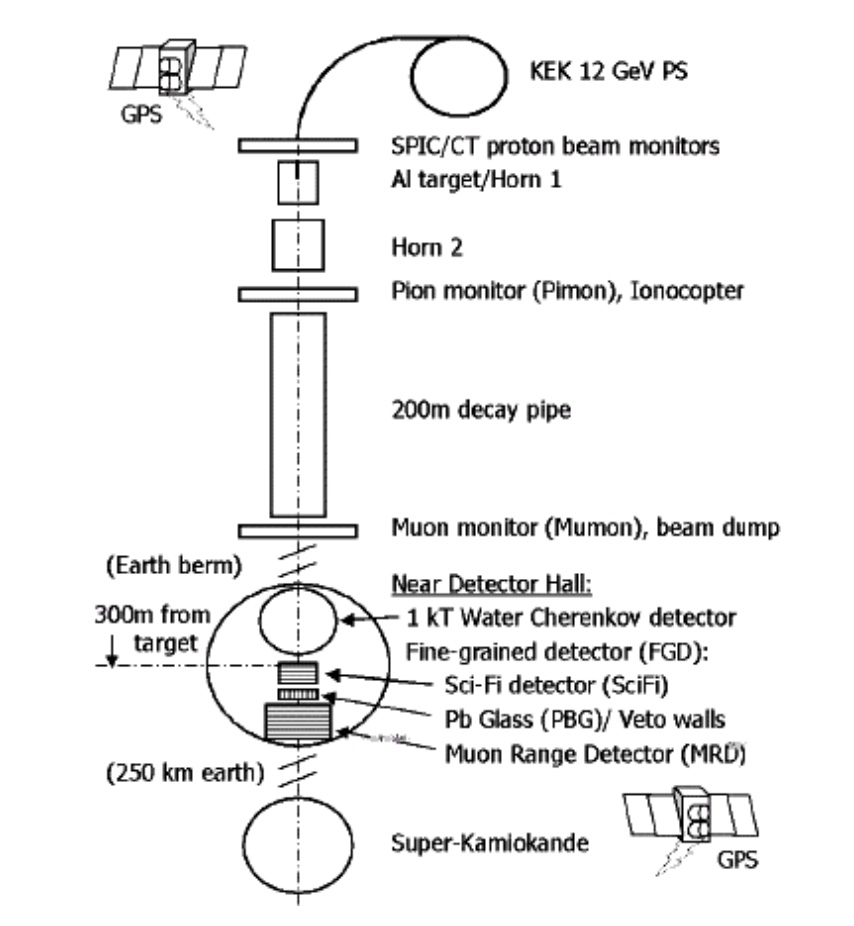
\includegraphics[width=0.5\textwidth]{figures/KEK.jpeg}
\vspace{2mm}
\caption{A schematic view of the K2K experiment Super-K~\cite{70K2K}.}
\label{fig:K2K}
\end{figure}

\subsection{MINOS}
%\url{http://www-numi.fnal.gov/Minos/minospub.txt}

The Main Injector Neutrino Oscillation Search (MINOS)~\cite{MINOS} is a muon neutrino disappearance experiment, consisting of one near (1km from the target) and one far detector (735km from the target) and using the NuMI~\cite{19NuMI} beam at Fermilab. 

The two detectors have been designed to be as similar as possible to minimize any systematic errors in comparing the observed neutrino spectra in the two detectors. They are both constructed of planes with two magnetised steal plates with a layers of scintillator in-between to measure charged particles and allow discrimination and of charge and measurement of the momentum. The far detector is composed of 486 octagonal plates with a diameter of 8 meters and total length of 30 meters providing a total mass of 5400 tons. The near detector contains only 282 planes, slightly squashed octagonal planes at 3.8 meters $\times$ 4.8 meters. MINOS showed results consistent with Super-Kamiokande and the K2K experiments. 

After MINOS the next step using the NuMI~\cite{19NuMI} beam is the NOvA~\cite{18nova} experiment, which is also an electron neutrino appearance experiment and hopes to be able to determine the mass hierarchy of neutrinos.

The MINERvA (Main INjector ExpeRiment $\nu$-A)experiment \cite{39minerva} will also use the NuMI~\cite{19NuMI} beam to study neutrino-nucleus scattering to improve models of neutrino-nucleus scattering to reduce systematic uncertainties in results from oscillation experiments.

MiniBooNE\cite{41MiniBooNE} continued on what was started by MINOS but had the principle aim on improving neutrino mass measurements.

\subsection{T2K}
\textbf{Correct after Pauls comments and add data.}

\textbf{Here or in chap 3?}

After the success of KEK, a similar baseline was constructed with the T2K-experiment\cite{21T2K},  a long-baseline neutrino oscillation experiment with a more powerful beam from the JPARC facility at Tokai to Super-Kamiokande, at a distance of 295 km with a near detector at hall 280 meters, in Tokai, from the target, see figure\ref{fig:T2K}

The neutrino beam comes from an initial 30 GeV/c proton beam which is passed through a horn fired onto a graphite target. After the target the secondary beam is passed through two magnetic horns and focused into a decay volume before passing the beam stopper. From here there is $\approx180$ meters of soil until hitting the near detector hall. This means that the near detector is comprised of only neutrinos with an expected flux as seen in \FigRef{fig:ND280Flux}. 

\begin{figure}[h!]
\centering
  \centering
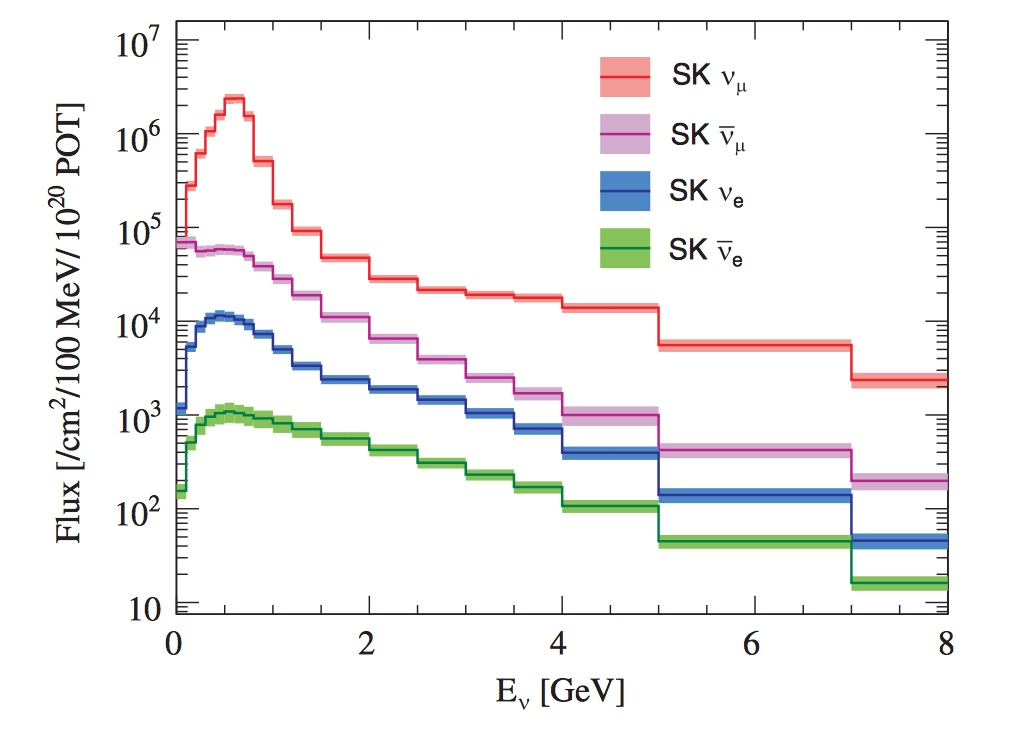
\includegraphics[width=\textwidth]{figures/ND280Flux.jpeg}
\vspace{2mm}
\caption{Simulated unoscillated expected neutrino fluxes for various flavours with expected systematic before applying near detector data plotted as bands. at Super-K~\cite{21T2K}.}
\label{fig:ND280Flux}
\end{figure}

\begin{figure}[h!]
\centering
  \centering
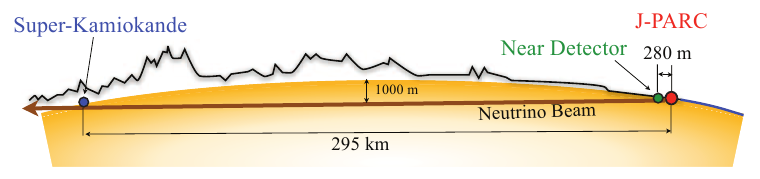
\includegraphics[width=\textwidth]{figures/T2KBeam.png}
\vspace{2mm}
\caption{A schematic view of the T2K experiment, including the near detector site ND280 and Super-K.}
\label{fig:T2K}
\end{figure}

The near detector hall contains two main experiments, an on-axis experiment INGRID and the off-axis ($2.5\deg$) ND280 detector both used to reduce model uncertainty and systematic uncertainty in the Super-Kamiokande analysis. \textbf{More details?}

The experiment wanted to improve the understanding of the neutrino oscillation parameters. T2K was able to successfully observe the appearance of muon to electron neutrino oscillations and find evidence that the third mixing angle $\theta_{13}$ is not zero. This is still an ongoing experiment. 

\begin{figure}[h!]
\centering
  \centering
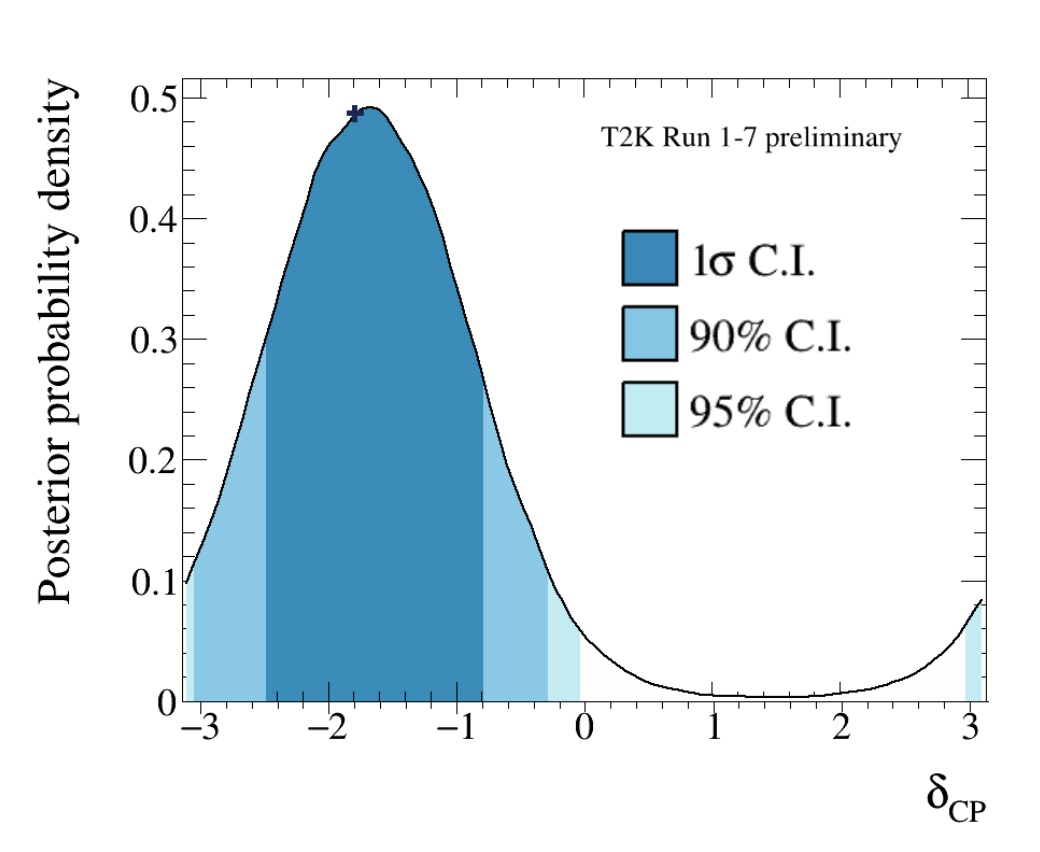
\includegraphics[width=0.7\textwidth]{figures/t2k1.jpeg}
\vspace{2mm}
\caption{Posterior probability density on $\delta$CP, where the cross represent the best-fit~\cite{T2Kfigures}.}
\label{fig:T2KCP}
\end{figure}

\begin{figure}[h!]
\centering
  \centering
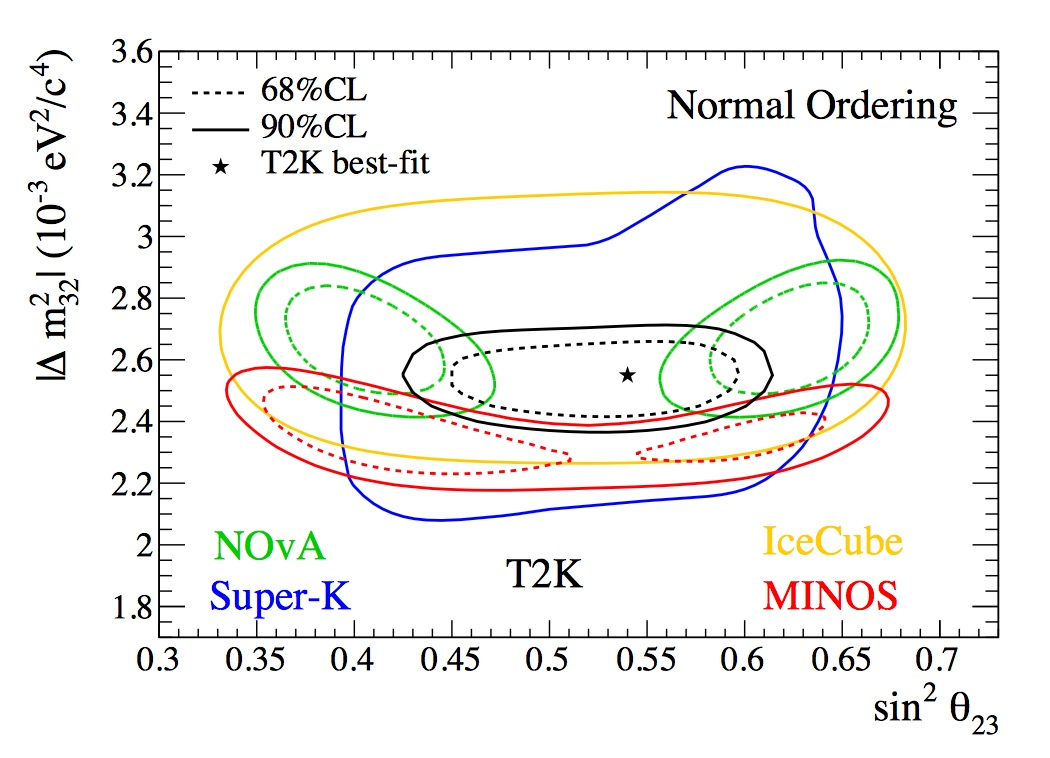
\includegraphics[width=0.7\textwidth]{figures/t2k2.jpeg}
\vspace{2mm}
\caption{The 90\% and 68\% confidence levels in the $\sin ^2 \theta_{23}-\Delta m^2_{32}$ space from T2K compared to other experiments, assuming normal ordering of neutrino masses~\cite{T2Kfigures}.}
\label{fig:T2K23}
\end{figure}

The main source of systematic error for T2K is caused by the difference of the target material and acceptance between the ND280 near detector (hydrocarbon) and the far detector water Cherenkov detector~\cite{T2Kpaper} motivating further studies and upgrades to the ND280 detector.

\section{Reactor}
Nuclear reactors are very intense sources of low energy neutrinos. Through beta-decay channels electron neutrinos are produced with well known energy spectra and low background. Compared to other neutrino sources the energy range is limited to below $9 MeV/c$, see \FigRef{fig:reactor} as well as a sharp cut of at $1.8 MeV/c$ required for inverse beta decay to occur. The low energy range means that oscillation experiments can be performed with a short baseline since equation~\ref{eq:twoPNeutrinoosc} provides the same probability by decreasing both the momentum and baseline.

\textbf{The positron deposits its kinetic energy to the scintillator then annihilates with an electron and generates two photons  which together with the deposited positron kinetic energy cause a so called prompt signal a few nanoseconds after the neutrino event.}


The low energy range also means that experiments based on reactor neutrinos can only search for $\bar{\nu_e}$ disappearance since the produced neutrinos do not have enough energy to produce muons or taus and any neutral current interaction will be very difficult to distinguish form background. Based on the current values neutrino reactor experiments are well suited to determine $\theta_{12}$ and $\Delta m_{12}^2 $ as well as  $\theta_{13}$ and $\Delta m_{13}^2$. Requiring specifically anti-neutrinos, becomes insensitive to $\delta_{CP}$ right?

\begin{figure}[h!]
\centering
  \centering
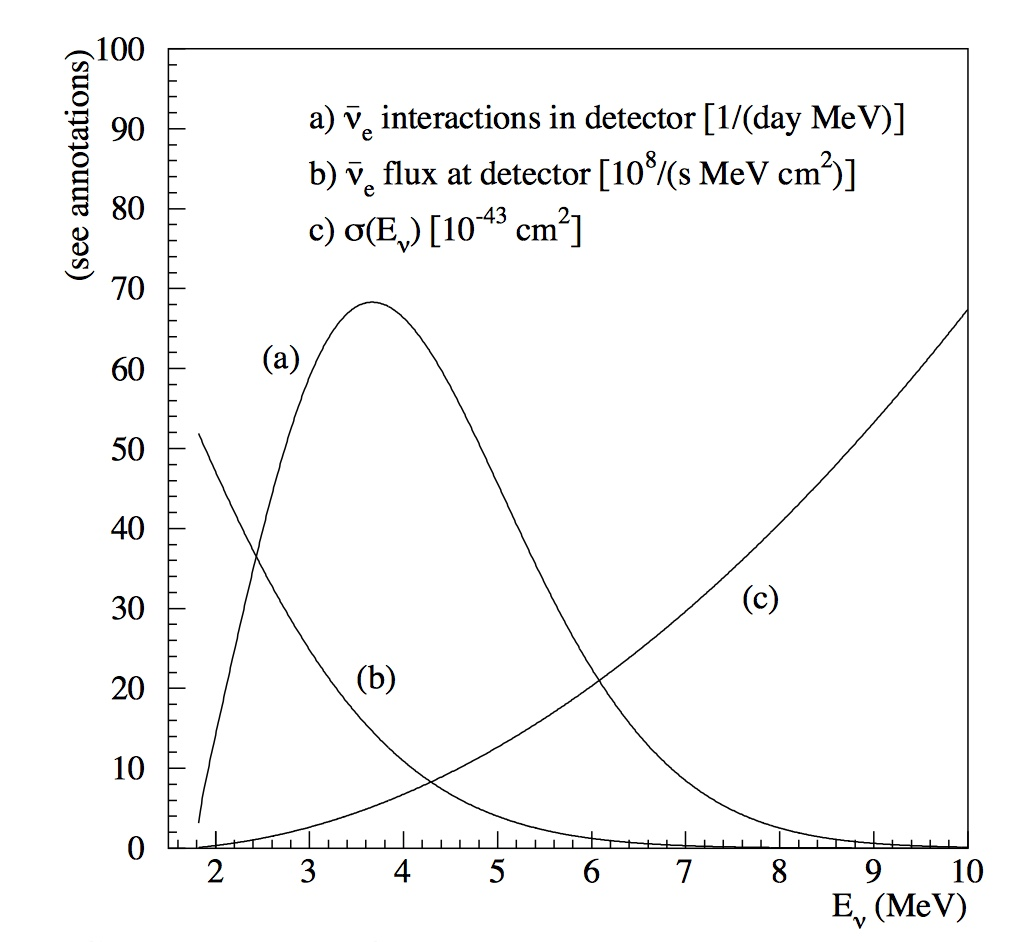
\includegraphics[width=0.7\textwidth]{figures/reactor.jpeg}
\vspace{2mm}
\caption{Energy spectrum of $\bar{\nu_e}$, the inverse beta decay cross section and interaction spectrum of detected inverse beta decay events~\cite{65Reactor}.}
\label{fig:reactor}
\end{figure}

\subsection{KamLAND}
After the completion of the KamiokaNDE experimental run the site used to install the Kamioka Liquid Scintillator Antineutrino Detector (KamLAND) in 2002. KamLAND, seen in \FigRef{fig:KamLAND}, looks specifically for neutrino oscillations by looking at anti electron neutrinos emitted from distant reactors~\cite{46KamLAND} by using a 1 kton liquid scintillator volume encased by oil. If the neutrinos interact with the volume by inverse beta-decay, it will produce positrons which will annihilate and produce two distinct photon signals, known as prompt signal.

The majority of the neutrino events are from 26 reactors within the distance range of 138-214 km providing a good baseline to see oscillations at the energy spectrum. The spectrum and results can be seen in \FigRef{fig:KamLAND2}. 

\begin{figure}[h!]
  \centering
  \begin{minipage}[b]{0.49\textwidth}
    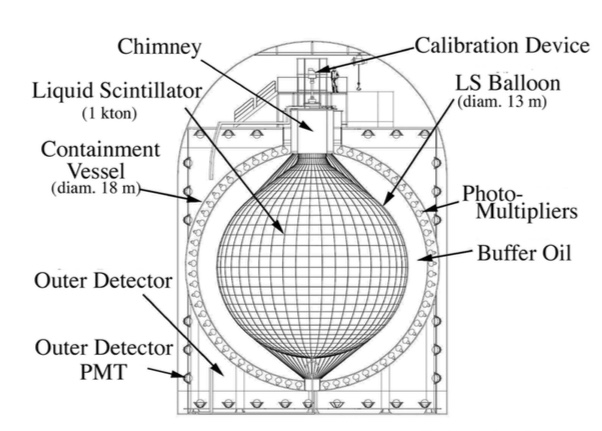
\includegraphics[width=\textwidth]{figures/KamLAND.jpeg}
    \vspace{2mm}
    \caption{Schematic diagram of the KamLAND detector~\cite{46KamLAND}.}
    \label{fig:KamLAND}
  \end{minipage}
  \hfill
  \begin{minipage}[b]{0.49\textwidth}
    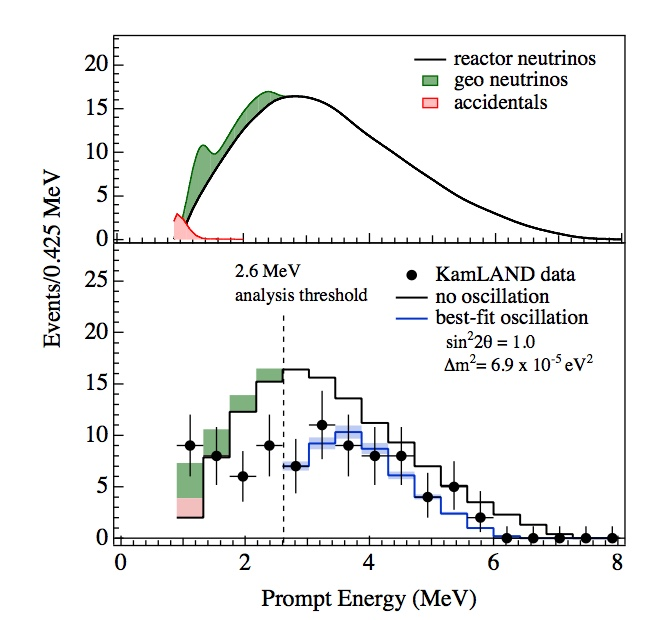
\includegraphics[width=\textwidth]{figures/KamLAND2.jpeg}
       \vspace{2mm}
    \caption{Top panel: Expected reactor $\bar{\nu_e}$ energy spectrum. Lower panel: Energy spectrum of the observed events along with the the no oscillation spectrum and best fit spectrum. }
     \label{fig:KamLAND2}
  \end{minipage}
\end{figure}

\subsection{Double Chooz}
The Double Chooz experiment~\cite{45DoubleChooz} started in 2004, used anti-neutrinos produced two nuclear cores from a nuclear power station to measure the neutrino mixing angle $\theta_{13}$ as well as showed that these detectors can be used to ensure non-proliferation~\cite{45DoubleChooz, 66ReactorNP}. The experiment consisted of two liquid scintillator detectors detectors at a distance of 280m and 1050m both consisted of PMTs inside a scintillating volume shielded from cosmic radiation. 

\begin{figure}[h!]
  \centering
  \begin{minipage}[b]{0.49\textwidth}
    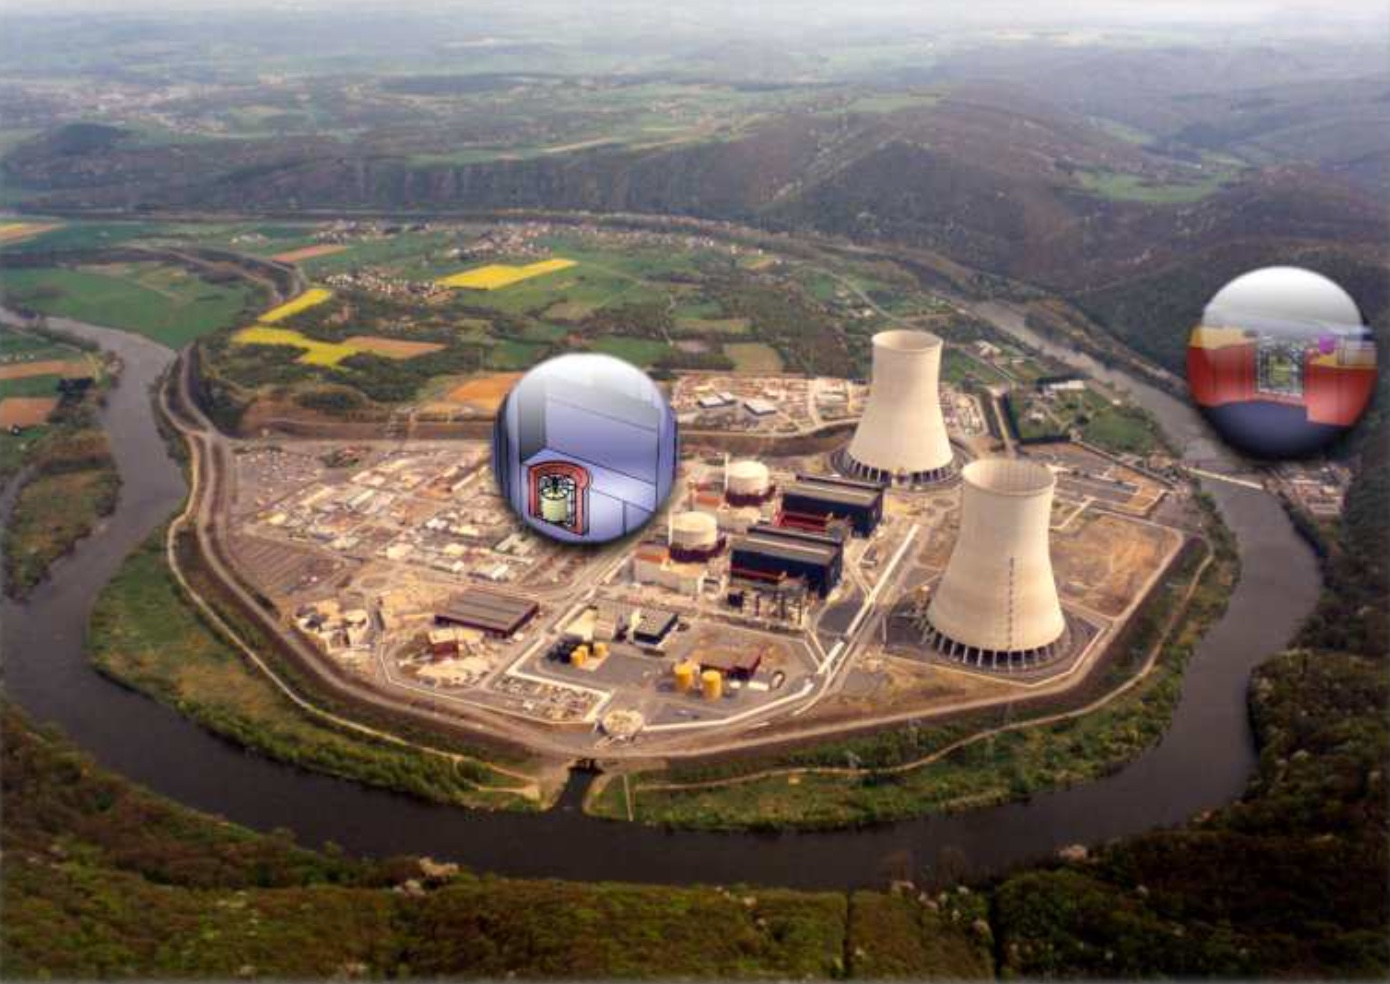
\includegraphics[width=\textwidth]{figures/doubleChooz.jpeg}
    \vspace{2mm}
    \caption{Overview of the Double Chooz experimental site~\cite{45DoubleChooz}.}
    \label{fig:dc}
  \end{minipage}
  \hfill
  \begin{minipage}[b]{0.49\textwidth}
    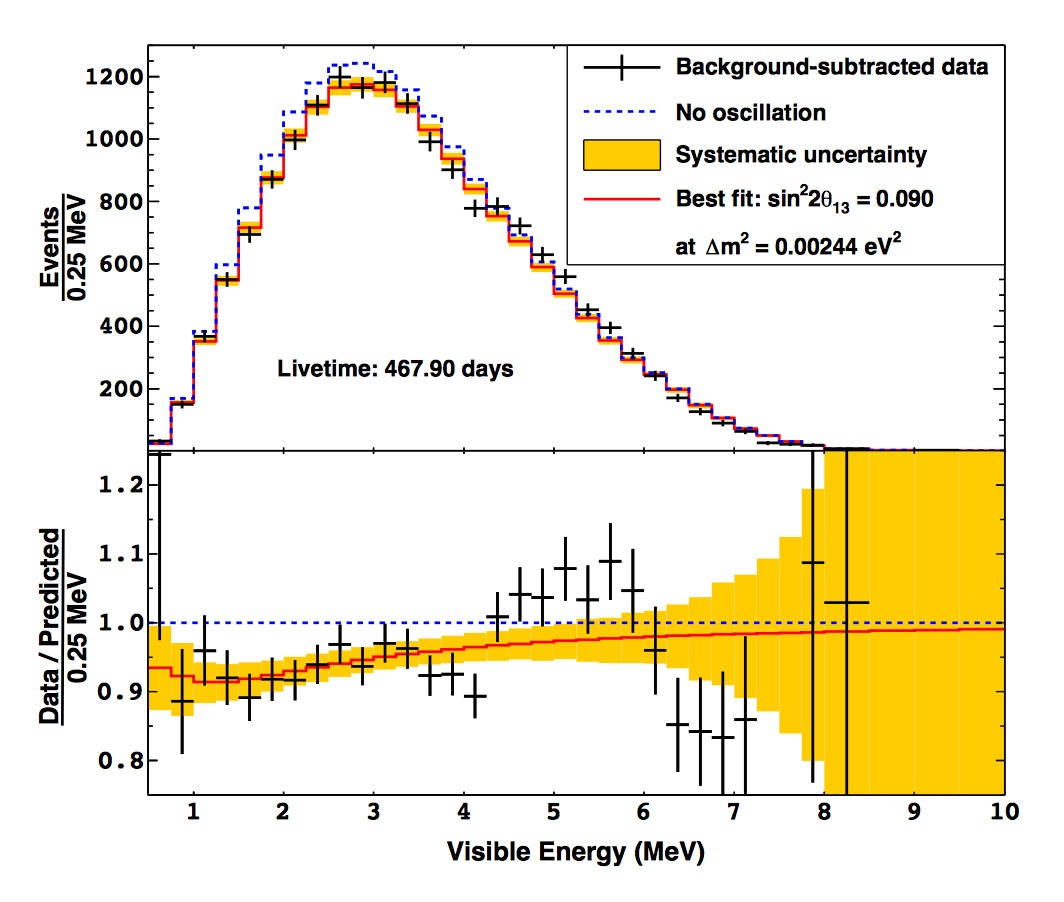
\includegraphics[width=\textwidth]{figures/doubleChooz2.jpeg}
       \vspace{2mm}
    \caption{Top panel: Measured energy spectrum with data on best fit and no oscillation models. Lower panel: Ratio of data over no-oscillation prediction~\cite{72Double}.}
     \label{fig:dc2}
  \end{minipage}
\end{figure}

\subsection{RENO}
The Reactor Experiment for Neutrino Oscillation (RENO), started taking data in 2011 and was the first experiment two use two identical detectors placed at a near and far site. The detectors are liquid scintillator detectors with 16.5 tons of Gadolinium doped scintillator. It measures neutrinos generated by six nuclear reactors each spread out perpendicular from a base line setting the detectors at 294 m and 1383 m from the center of the base line, see~\FigRef{fig:reno1}. Reno measured $|\Delta m^2_{32}| = 2.61 \pm 0.16 \pm 0.09 \times 10^{-3} eV^2$ and $\sin^2(2\theta{13}) = 0.086 \pm 0.006 \pm 0.005$ using the data in~\FigRef{fig:reno2}.

\begin{figure}[h!]
  \centering
  \begin{minipage}[b]{0.49\textwidth}
    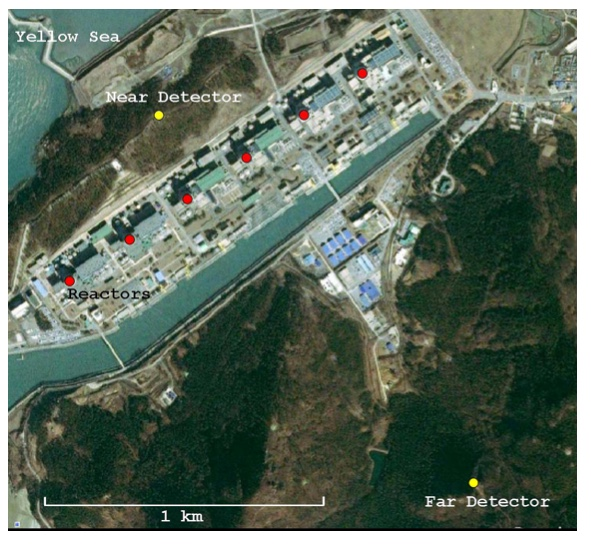
\includegraphics[width=\textwidth]{figures/reno1.jpeg}
    \vspace{2mm}
    \caption{Layout of the RENO detectors, yellow and reactors in red. The six reactors are equally spaced in a 1280 m span~\cite{73Reno}.}
    \label{fig:reno1}
  \end{minipage}
  \hfill
  \begin{minipage}[b]{0.49\textwidth}
    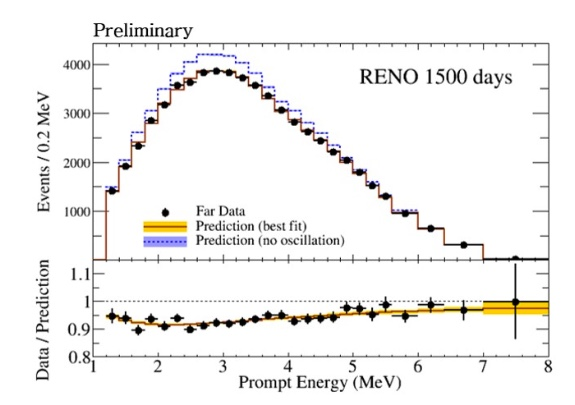
\includegraphics[width=\textwidth]{figures/reno2.jpeg}
       \vspace{2mm}
    \caption{Top panel: Measured energy spectrum with data on best fit and no oscillation models. Lower panel: Ratio of data over no-oscillation prediction~\cite{73Reno}.}
     \label{fig:reno2}
  \end{minipage}
\end{figure}

\subsection{Daya Bay}
\textbf{Correct after Pauls comments and add data.}

The Daya Bay experiments~\cite{44DayaBay} main goal is to improve the measurement of $\theta_{13}$It is improving results from Double Chooz by utilizing eight identical detectors placed at three locations around the Daya Bay area consisting of a total of 6 different nuclear cores. This layout allows for maximum sensitivity and the ability to reduce systimatic uncertainties due to uncertainties in reactor power levels. It also allows for cross-calibration of the detectors since they are all identical. Each detector is a segmented Gadolinium doped liquid scintillator detector using PMTs to read out photons produced through inverse beta-decay and annihilation. The experiment has been taking data since 2011.

\begin{figure}[h!]
  \centering
  \begin{minipage}[b]{0.49\textwidth}
    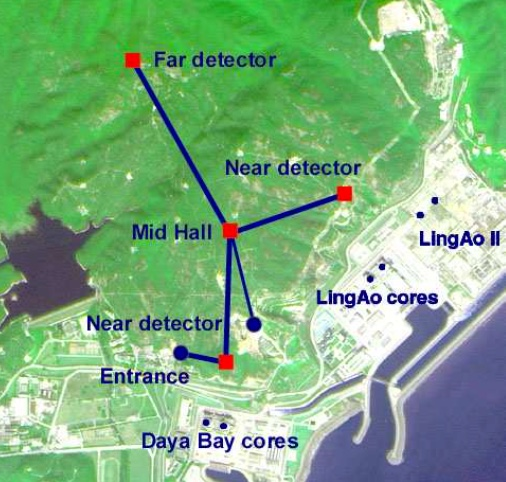
\includegraphics[width=\textwidth]{figures/DayaBay.jpeg}
    \vspace{2mm}
    \caption{Layout of the Daya Bay experiment~\cite{44DayaBay}.}
    \label{fig:DB}
  \end{minipage}
  \hfill
  \begin{minipage}[b]{0.49\textwidth}
    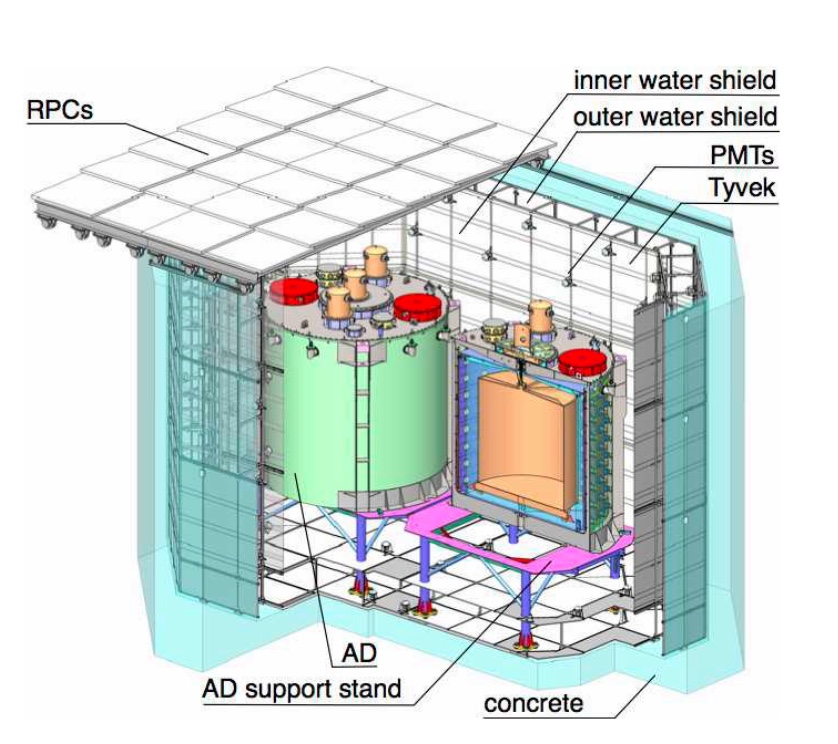
\includegraphics[width=\textwidth]{figures/db2.jpeg}
       \vspace{2mm}
    \caption{Near site layout of the Daya Bay detector with surrounding structure~\cite{74DayaBay}.}
     \label{fig:db2}
  \end{minipage}
\end{figure}

\begin{figure}[h!]
  \centering
  \begin{minipage}[b]{0.49\textwidth}
    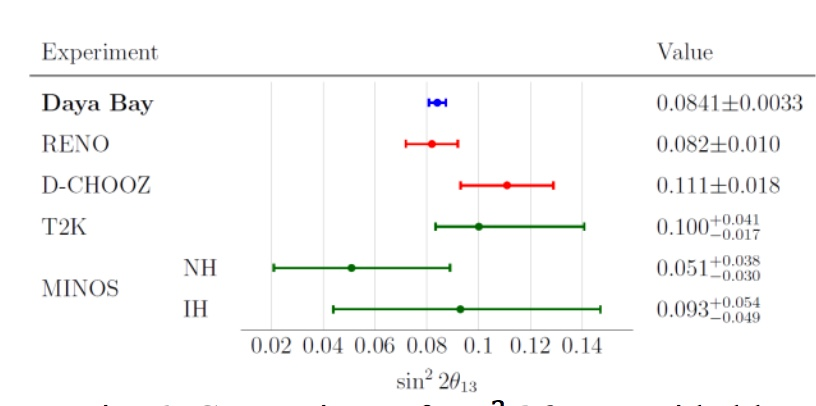
\includegraphics[width=\textwidth]{figures/db3.jpeg}
    \vspace{2mm}
    \caption{Comparison of $\sin^2 2\theta_{13}$ measurements from various experiments, taken from~\cite{74DayaBay}.}
    \label{fig:db3}
  \end{minipage}
  \hfill
  \begin{minipage}[b]{0.49\textwidth}
    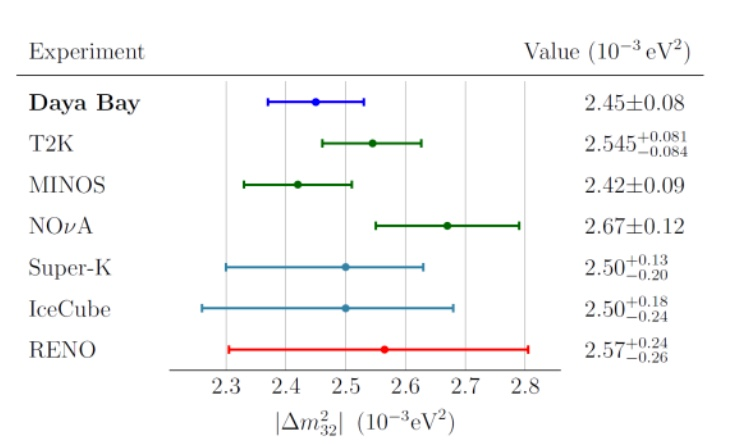
\includegraphics[width=\textwidth]{figures/db4.jpeg}
       \vspace{2mm}
    \caption{Comparison of $|\Delta m^2_{32}|$ measurements from various experiments, taken from~\cite{74DayaBay}.}
     \label{fig:db4}
  \end{minipage}
\end{figure}

\subsection{JUNO}

The Jiangmen Underground Neutrino Observatory (JUNO)~\cite{75Juno} is a 20 kton liquid scintillator detector currently under construction and aiming to start data taking in 2020, seen in both \FigRef{fig:juno1} and \FigRef{fig:juno2}. It has as one if its primary aim to determine the mass hierarchy, sign of the mass splitting, using reactor neutrinos and inverse beta-decay with an improved energy resolution compared to previous experiments~\cite{75Juno}. It uses the Daya Bay reactor as a far reactor and results from the Daya Bay experiment to reduce systematic errors from the reactor.

\begin{figure}[h!]
  \centering
  \begin{minipage}[b]{0.49\textwidth}
    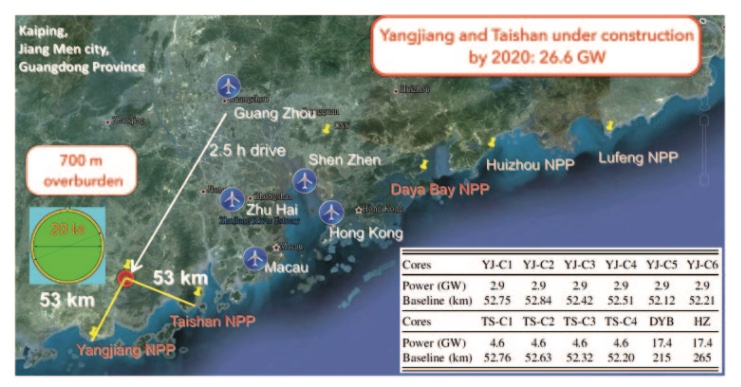
\includegraphics[width=\textwidth]{figures/juno1.jpeg}
    \vspace{2mm}
    \caption{Location of the JUNO site with distances to the near by reactors, Yangjiang and Taishan at both 53km as well as Daya Bay at 215km away.~\cite{75Juno}.}
    \label{fig:juno1}
  \end{minipage}
  \hfill
  \begin{minipage}[b]{0.49\textwidth}
    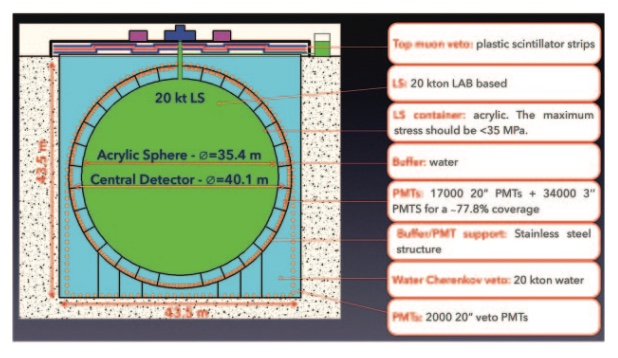
\includegraphics[width=\textwidth]{figures/juno2.jpeg}
       \vspace{2mm}
    \caption{Schematic view of the JUNO detector~\cite{75Juno}.}
     \label{fig:juno2}
  \end{minipage}
\end{figure}


\section{Future neutrino oscillation experiments}

\subsection{DUNE}
LBNF/DUNE\cite{23DUNE}, seen in \FigRef{fig:dune2}, is a new experiment currently under construction aiming at looking at the full range of $\delta_{cp}$ with greater sensitivity than before by improving on the MINOS~\cite{MINOS} experiment, and performing an electron neutrino appearance measurement with a high-powered neutrino beam from Fermilab and a 40 kton liquid argon detector at a distance of 1300 km, in the Homestake mine in South Dakota with a full initial physics study presented in~\cite{76Dune}

The main goals are to perform precision measurements of neutrino oscillation to determine $\delta_{CP}$ within $5\sigma$, determining the neutrino mass ordering, seen in \FigRef{fig:dune1}, and measuring the sign of the mixing angle $\theta_{23}$ all to within new limits. 

\begin{figure}[h!]
  \centering
  \begin{minipage}[b]{0.49\textwidth}
    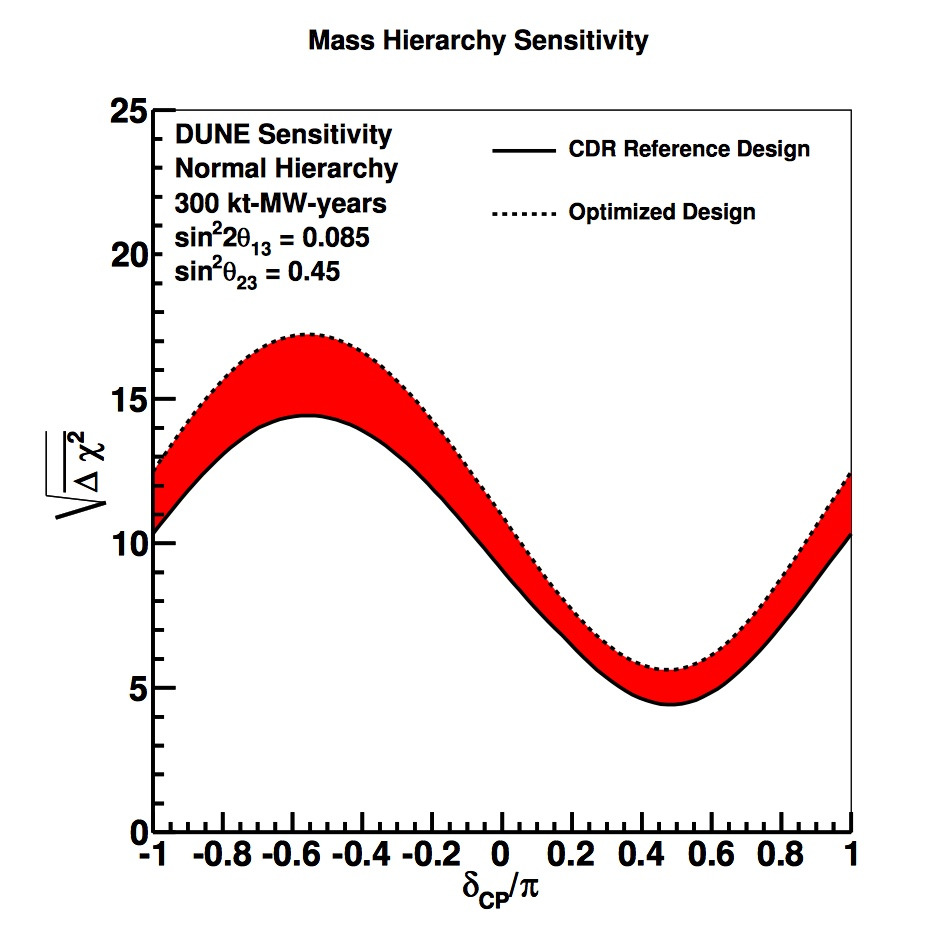
\includegraphics[width=\textwidth]{figures/dune2.jpeg}
    \vspace{2mm}
    \caption{Estimated significance of the mass hierarchy discrimination metric as a function of values for $\delta_{CP}$ ~\cite{23DUNE}.}
    \label{fig:dune1}
  \end{minipage}
  \hfill
  \begin{minipage}[b]{0.49\textwidth}
    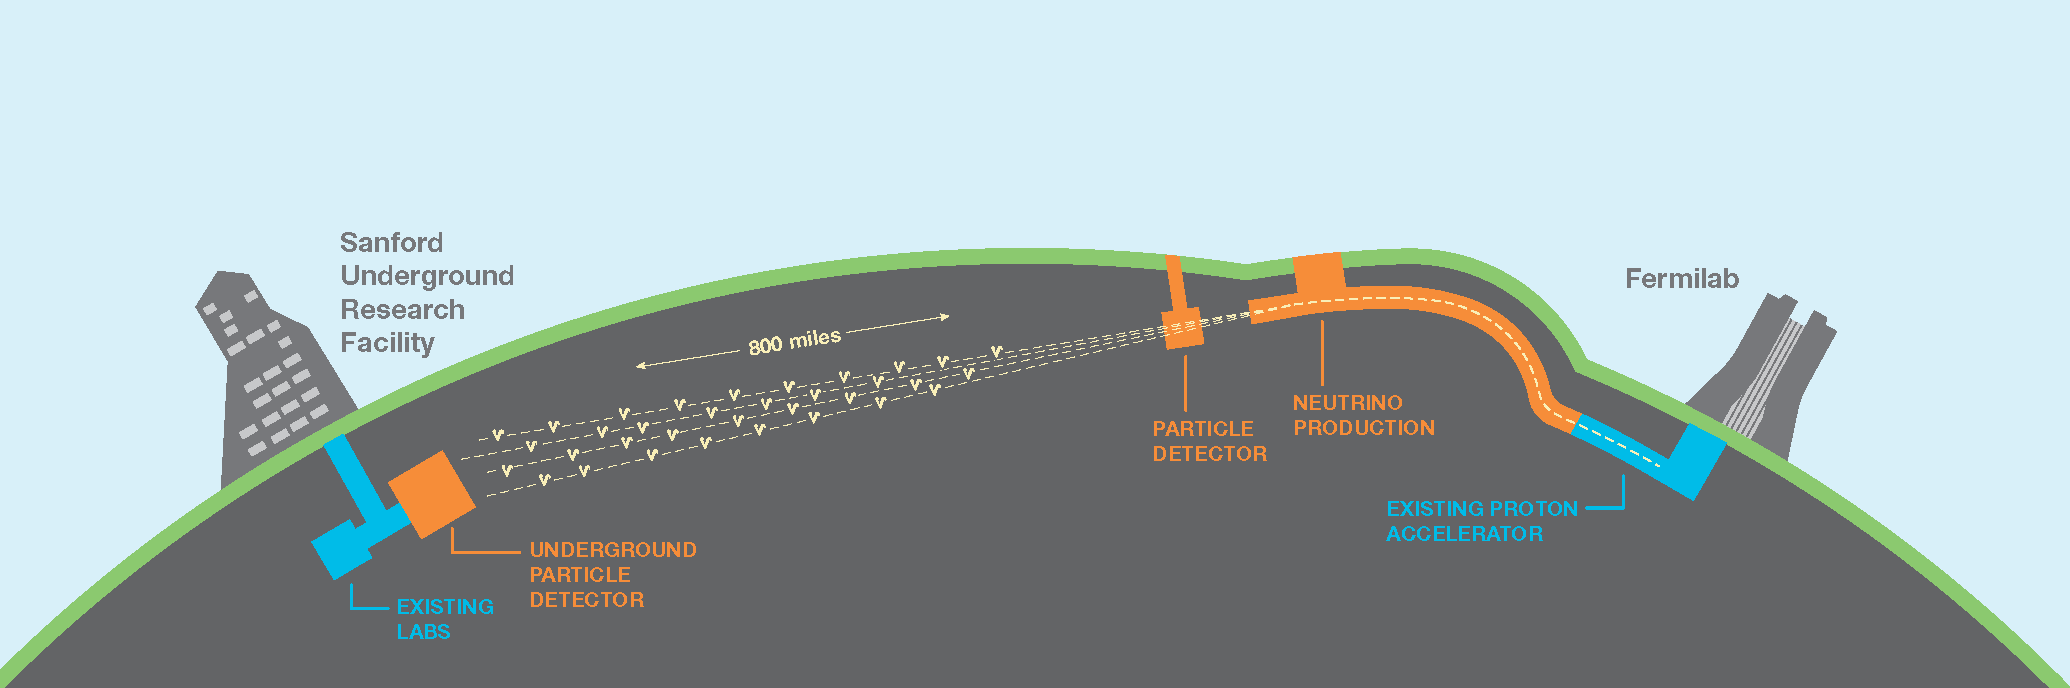
\includegraphics[width=\textwidth]{figures/dune.png}
       \vspace{2mm}
    \caption{Schematic view of the DUNE detectors~\cite{23DUNE}.}
     \label{fig:dune2}
  \end{minipage}
\end{figure}

\subsection{Hyper-K}

The Hyper-Kamiokande Experiment (Hyper-K)\cite{24HyperK}  builds on the T2K-experiment\cite{21T2K} by improving the neutrino beam at JPARC, and expanding the water Cherenkov detector by a factor of 10 to a fiducial volume of 500 ktons, which aims to improve the sensitivity for $\delta_{CP}$ and determine the value within $>3\sigma$, and $<18^\circ$ and determine the mass hierarchy within $>3\sigma$ and the sign of $\theta_{23}$ with a $>90\%$ confidence level.

\begin{figure}[h!]
  \centering
  \begin{minipage}[b]{0.59\textwidth}
    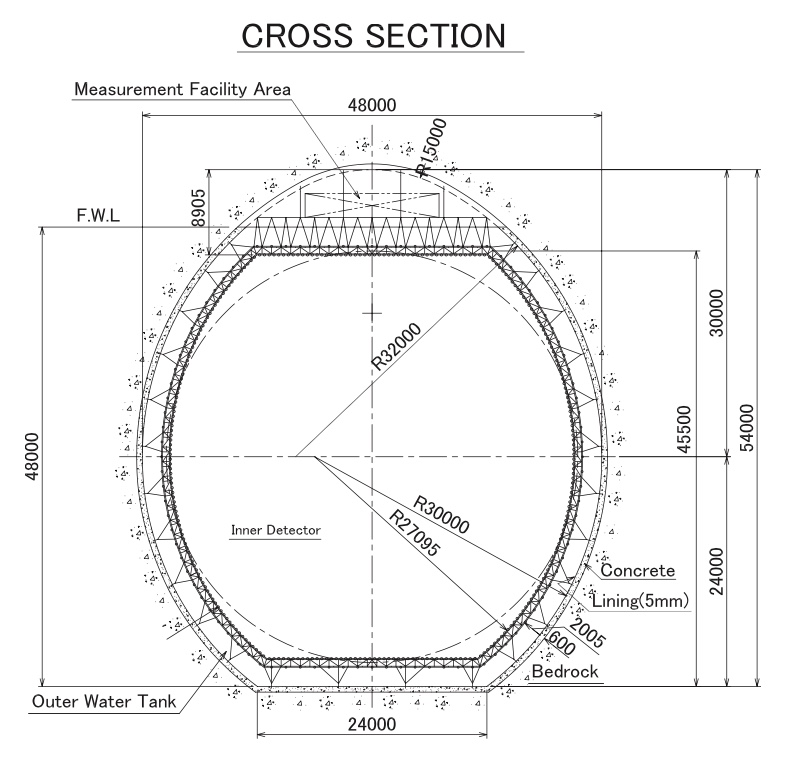
\includegraphics[width=\textwidth]{figures/hyper1.jpeg}
    \vspace{2mm}
    \caption{Cross section view of the Hyper-Kamiokande detector~\cite{24HyperK}.}
    \label{fig:hyper1}
  \end{minipage}
  \hfill
  \begin{minipage}[b]{0.39\textwidth}
    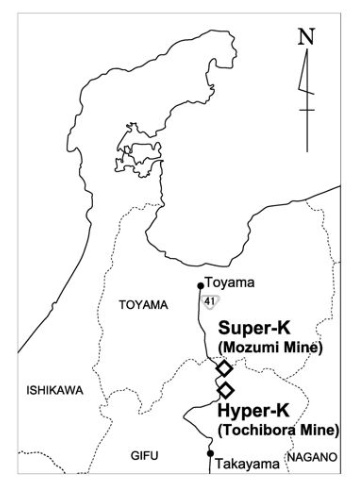
\includegraphics[width=\textwidth]{figures/hyperk2.jpeg}
       \vspace{2mm}
    \caption{A map showing the proposed candidate site~\cite{24HyperK}.}
     \label{fig:hyper2}
  \end{minipage}
\end{figure}

\section{Neutrino Factory}\label{subsec:nuFACT}
The Neutrino Factory (NuFACT) is a novel concept for a neutrino accelerator which will produce a high intensity (1000 higher than previously) and high energy beam (up to 15 GeV~\cite{Fix7}). Compared to other previous experiments it will produce a two flavour, electron and muon, neutrino beam through a muon decay ring. The neutrino factory has the capacity to improve the precision of neutrino oscillation measurements, since the neutrino beam from the decay of muons can be determined with high accuracy. The beam produces one bunch of $\mu^+$ and one bunch of $\mu^-$, so the facility can make measurements of $\nu_{\mu}$ and $\bar{\nu_{e}}$ and $\bar{\nu_{\mu}}$ and $\nu_{e}$ simultaneously. Using this $\delta_{cp}$ can be decisively explored, with an expected accuracy of $\Delta \delta_{CP}\sim 5^\circ$~\cite{25NUfact}. A schematic of the facility is shown in figure \ref{fig:nuFact} showing the full accelerator chain. The full chain, starts by producing muons and pions from a proton beam on target. Pions are then captured in a strong solenoid magnetic field surrounding the target. The bunches are sent rhough the so called Front end containing a phase rotation and a ionisation cooling channel before being re-accelerated and entering the muon storage ring. Before entering the ring the muons are charge separated and go into the storage ring in counter-rotating directions. After $\approx 70$ turns of the circuit the muons decay through the following modes with the branching ratio:

%The muon beam is then cooled to focus the beam before further accelerating the muon beam to its final energy and introducing it into the decay ring. 

\begin{align}
\mu^- &\rightarrow e^- + \bar{\nu_e} + \nu_\mu, \approx 100\% \\
\mu^- &\rightarrow e^- + \bar{\nu_e} + \nu_\mu + \gamma, <1\% \\
\mu^- &\rightarrow e^- + \bar{\nu_e} + \nu_\mu + e^+ + e^-, <1\%
\end{align}

From the branching ratio the energy spectrum and composition of the neutrino beam is well known as the decays only produces two different neutrino flavours. It is important to note that a $\mu^+/mu^-$ beam will produce $\bar{\nu_\mu} + \nu_e / \nu_{\mu} + \bar{\nu_e}$. Thus for a $\mu^-$ beam any electron neutrinos or anti-muon neutrinos discovered must have been produced through oscillation. To be able to distinguish muons from anti-muons at a detector, a magnetic field is required motivating the design of any considered detector, described in subsection~\ref{subsec:MINDdetector}. Currently there are proposals for NuFACT to be constructed at CERN~\cite{25NUfact}, ESS~\cite{ESS} and FERMILAB~\cite{NuFACTfermi}, where it is also seen as a step toward a full muon collider experiment.
%Neutrino factory, explain it. MIND detector for nufact.  MIND needed for charge id, wrong sign muons produced from mu neutrino and anti electron neutrino in accelerator, anti electron to anto muon oscillation. Nufact known 0 anti nu mu in generation, only in oscillation. Prob is 0 for nufact for wrong sign at near detector/source.

\begin{figure}[h!]
\centering
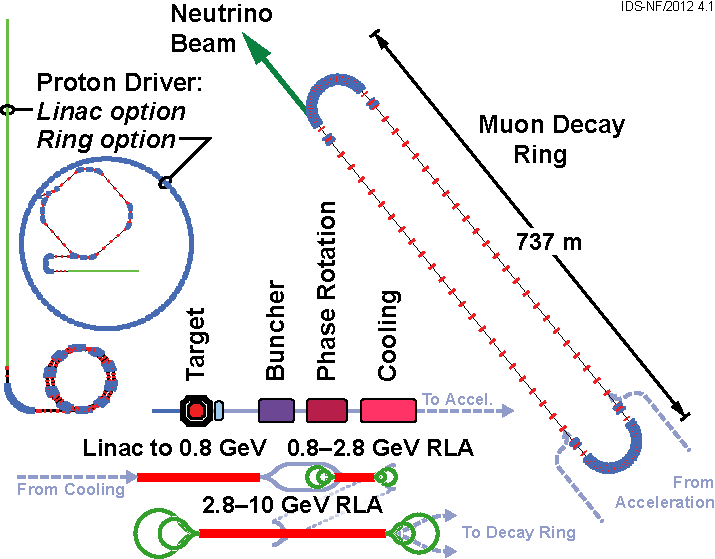
\includegraphics[width=0.9\textwidth]{figures/131112-IDS-NF.pdf}
\caption{Schematic diagram of the Neutrino Factory~\cite{Fix7}.}
\label{fig:nuFact}
\end{figure}

\begin{figure}[h!]
\centering
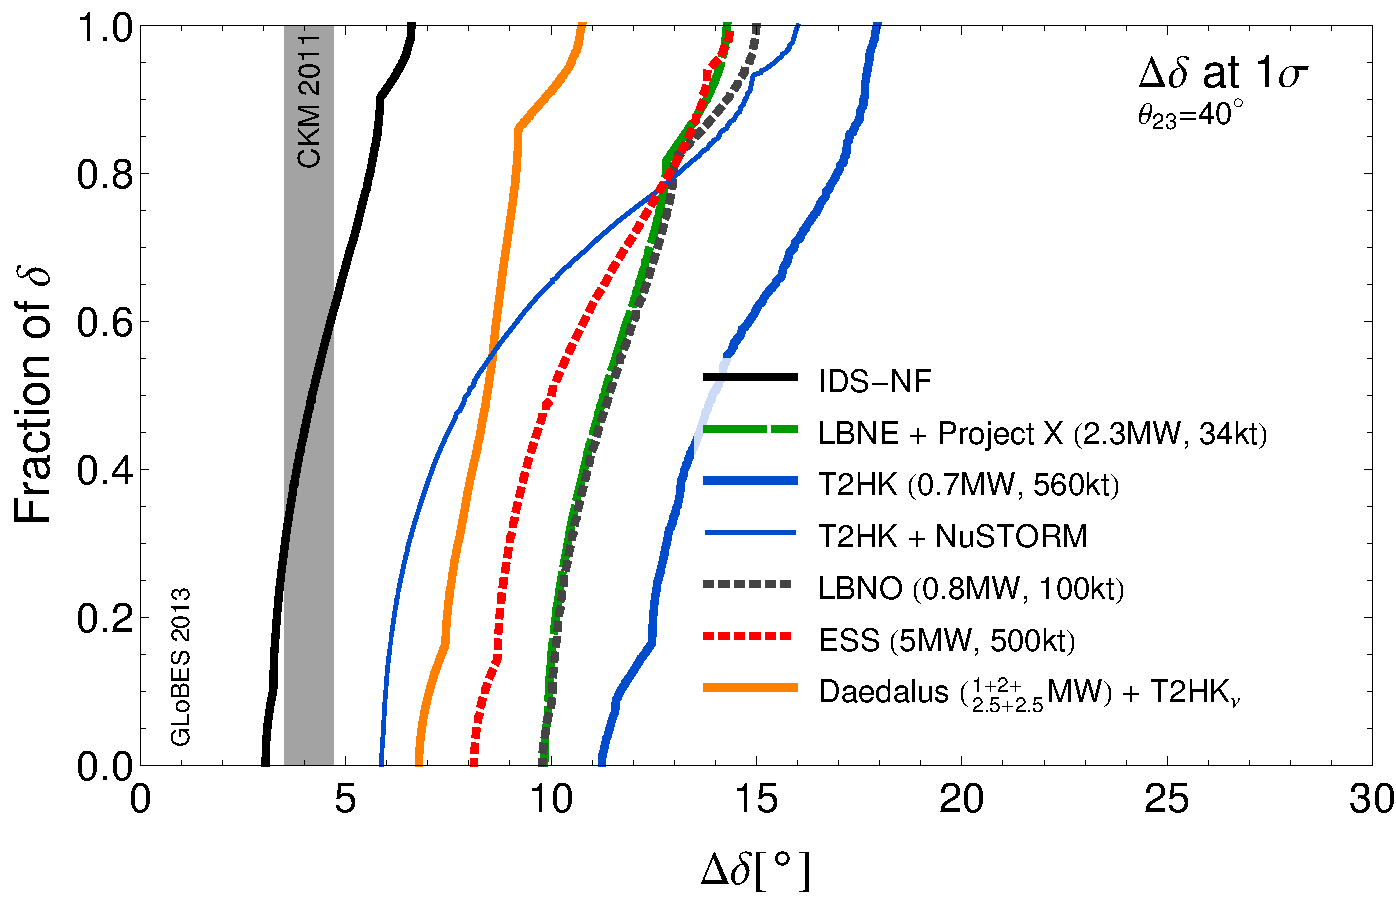
\includegraphics[width=0.9\textwidth]{figures/rdr-cp-precision-comparison-131216.pdf}
\caption{Expected precision for a measurement of the $\delta_{cp}$ at a Neutrino Factory compared to alternate neutrino oscillation facilities~\cite{Fix7}.}
\label{fig:nuFactExp}
\end{figure}


\textbf{Add in different channels and how it requires a charge identification to be able to identify the various challenge.}

\subsection{NuStorm}

The Neutrino Factory is a complex and expensive facility which requires new technology to be realised. To overcome this a staged approach has been suggested, where each stage would be delivering physics~\cite{Fix7}. The first state in this plan is named nuSTORM (Neutrinos from Stored Muons) with a schematic shown in figure~\ref{fig:nuStorm}. The nuSTORM beam is designed to produce 3.8 GeV/c muons which are injected into a muon storage ring. Compared to the full neutrino factory nuSTORM is expected to have some pions and kaons for the first pass in the storage ring providing some contamination in the final beam producing both neutrinos and anti-neutrinos for both muon and anti-muon modes and thus a near detector is required to measure the flux of both. 

\begin{figure}[h!]
\centering
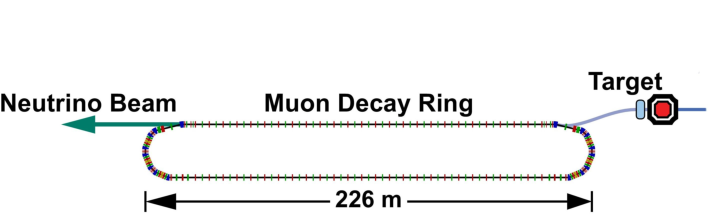
\includegraphics[width=\textwidth]{figures/nuSTORM_schematic.pdf}
\caption{A schematic of a nuSTORM facility~\cite{Fix7}.}
\label{fig:nuStorm}
\end{figure}

For the both NuFACT and nuSTORM the detector type proposed will be a MIND type, similar to the ones used in CDHSW and MINOS~\cite{NuFACTIDS}.

~\cite{77nustorm}.

\section{Magnetized Iron Neutrino Detectors}\label{subsec:MINDdetector}
\textbf{Correct after Pauls comments and add data.}

Magnetized Iron Neutrino Detectors (MINDs) have been operated in several experiments such as CDHSW~\cite{40CDHSW} and MINOS~\cite{MINOS}. This type of detector, with magnetized steel plates and scintillation plates, is well suited to provide large mass for neutrino experiments and is able to provide momentum measurements by using range and curvature calculations as well as providing charge identification. A MIND type detector has been selected as the baseline detector for a neutrino factory~\cite{ISS, 27Bross}, since it is the cheapest and most effective way of producing a large magnetized volume. This has provided the motivation for creating a prototype detector to perform a number of studies.

Since water Cherenkov and liquid argon detectors have been established or actively studied for future very large scale neutrino oscillation experiments, a MIND type detector is not foreseen to be used as the main interaction medium for any planned upcoming experiments.. A MIND type detector can however be used to provide charge identification of muons if positioned downstream of any neutrino target which is not magnetized.


\textbf{OLD}

\subsubsection{IceCube}
The IceCube observatory~\cite{43IceCube} also exploits the fact that particles produced in neutrino interactions emit Cherenkov photons. The low interaction probability of neutrinos require a large interaction volume. The South Pole offers a large interaction volume with very good optical qualities, using this is possible to instrument cubic kilometres of ice with a rather sparse spacing of detectors. The basic detection unit in IceCube is the digital optical module (DOM). The DOM contains, amount other things a PMT encapsulated in a glass pressure sphere to withstand the extreme pressure in the deep ice. In total 5160 DOMS are deployed, instrumenting a volume of one cubic kilometre of ice and allowing detection of astrophysical neutrinos in the energy range of TeV to PeV.

\begin{figure}
\centering
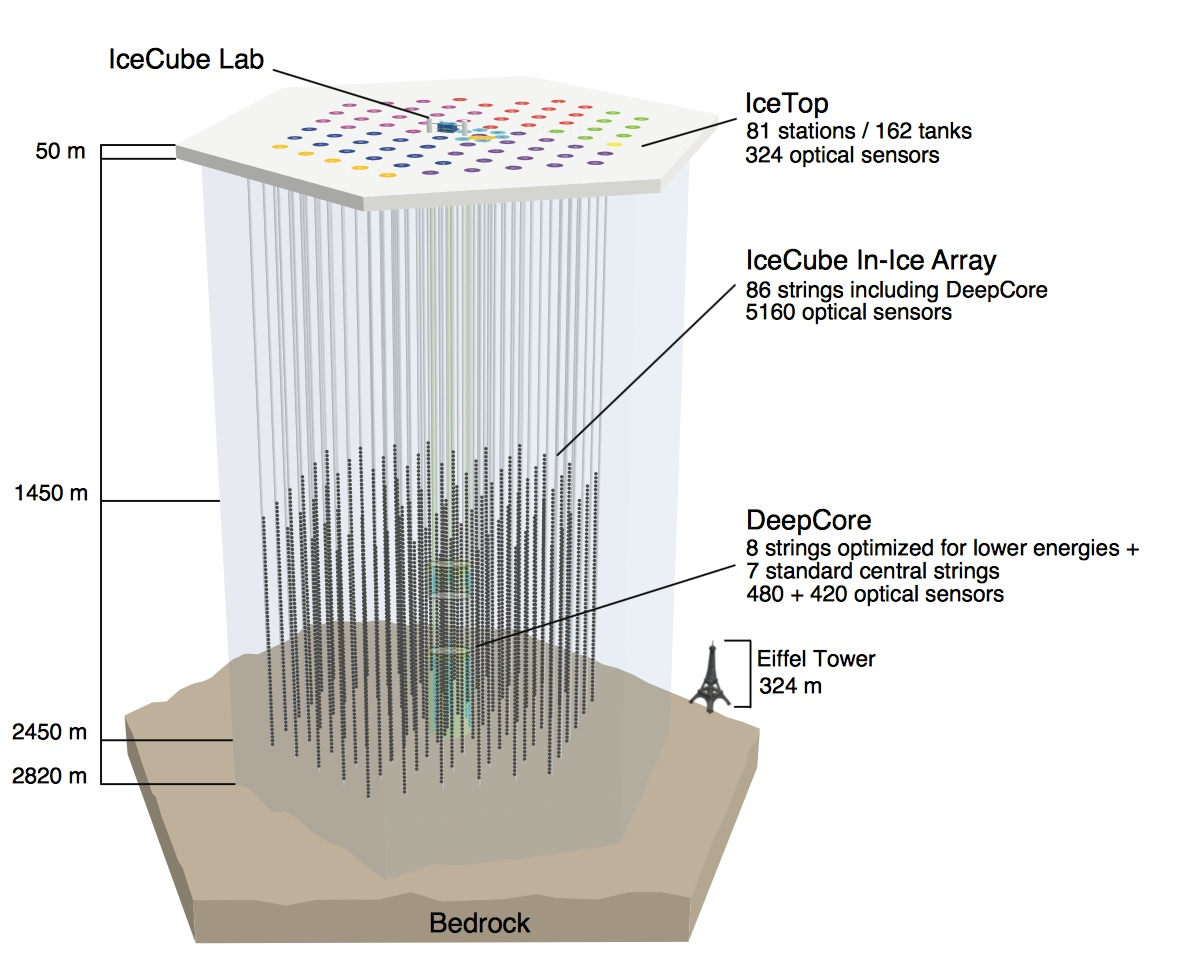
\includegraphics[width=.5\textwidth]{figures/IceCube.jpeg}
\caption{The IceCube Neutrino Observatory}
\end{figure}







%==============================================================================


% -----------------------------------------------------------------------------
% Main stuff.

\chapter{Baby MIND + WAGASCI}
\label{c:WAGASCI}

%Initially MIND prototype for nufact, now low pt can be used as muon spectrometry. Add preface to describe what done by xyz, clarify my contribution.
\section{Baby MIND/NP05}


%http://cds.cern.ch/record/2057587/files/SPSC-P-353.1.pdf

%Magnetized Iron Neutrino Detectors (MIND) have been operated in several experiments spanning 4 or so decades, such as CDHS, MINOS. These structures with magnetized steel plates interleaved with detector mod- ules are particularly well suited to provide large mass for neutrino experiments, and the characterization of the outgoing muon from νμ interactions, providing momentum measurements both by range and curvature, so in a sense self-calibrating, and providing charge identification. For this reason they have been naturally selected as baseline neutrino factory detectors.

%The Baby MIND project was launched as a prototyping activity within the European Commission-funded AIDA project with the principal aim to study muon charge identification efficiencies. The requirements that were set were correct sign background rejection to identify the wrong sign muon signature of a neutrino oscillation event at a Neutrino Factory.

 %In order to extend the neutrino factory capability to wrong- sign electrons, studies were made of totally active scintillator detectors (TASD) immersed in large volume magnetic field, in which sufficient tracking for electrons would allow charge separation. Since the scintillating detectors for the MIND and TASD are the same, the AIDA project foresaw to build a TASD prototype, immerse it in a large magnet available at CERN, and expose it to an electron beam.
 
%A MIND is planned for the recently approved WAGASCI experiment (T-59) at J-PARC on the T2K beamline to improve measurements of the ratio of neutrino interaction cross-sections on water and carbon motivated by the need to reduce systematics due to nuclear effects in water, currently the dominant systematic uncertainty in the T2K neutrino oscillation analyses. The size of the Baby MIND is particularly well suited for the WAGASCI experiment providing excellent acceptance for forward secondaries from interactions in the upstream WAGASCI water and carbon targets, Figure 1. The Baby MIND will be constructed and tested on a charged particle beamline at CERN. Once fully characterized, it will be shipped to J-PARC for operation with the WAGASCI experiment, where it is commonly referred to as the downstream Muon Range Detector (dMRD). Charge identification at much lower muon momenta in the T2K beamline is addressed by increasing the resolution on measurements of particle track angle rather than only providing position information.


%Magnetised Iron Neutrino Detectors (MINDs) have been proposed for Neutrino Factories, since wrong-sign muons are the neutrino oscillation signal. Baby MIND is a prototype detector to study charge identification of muons on a charged particle beamline at CERN. The CERN Neutrino Platform approved Baby MIND as experiment NP05 in December 2015 and construction started in August 2016 and finished in June 2017. 

The prototype Magnetized Iron Neutrino Detector (Baby MIND)~\cite{26babyMIND} was designed with the aim to study muon charge identification efficiencies in order to get estimates for a future Neutrino Factory, discussed in this section. The Baby MIND project was launched as a prototyping activity within the European Commission-funded AIDA-2020 project. The particle charge is essential for their oscillation measurements since wrong-sign muons are the neutrino oscillation signal. During the design process a secondary aim was added, to measure the momentum and charge of muons from neutrino interactions in water and hydrocarbon targets at the J-PARC T59 WAter-Grid-SCIntilator-detector (WAGASCI) experiment, further discussed in section~\ref{sec:WAGASCI}

The Baby MIND collaboration is comprised of around 46 scientists from 10 different institutions, and is part of the CERN Neutrino Platform as experiment NP05~\cite{Fix2} and is as of 2018 fully integrated into WAGASCI and in turn T2K.

\subsection{Motivation}

The Baby MIND aims to show that MIND type detectors are viable to use for muon charge identification at low momenta ($<1$GeV/c) and also to show how well the charge can be identified from a Neutrino Factory~\cite{25NUfact} beam. A secondary motivation is to act as a platform to test new electronics, scintillation fibres and data acquisition for future experiments. Additionally the experiment aims to compare simulations from GEANT4~\cite{Geant4} to data taken from the detector to be able to verify the properties of muon interactions at momentum ranges of 0.5 to 10 GeV/c. Separating and identifying particles of different charges requires a magnetic field, and to perform identification at low momenta a high uniform field has to be created in a large volume and preferably without fully stopping the particles which are being identified. 
The main difficulty that arises is to magnetise the volume in an inexpensive and simple manner.

In essence one has to balance having a large magnetized volume over for instance gas, which will not stop particles but it will not be strong/cheap/large or uniform over the other option of magnetising a large iron block which is cheap and uniform but stops particles.

For the Baby MIND a novel approach was chosen to use thin high quality magnetised ARMCO steel plates in an arrangement to optimize charge identification while minimizing the amount of steel plates interspersed with scintillator modules. The optimal design has been slightly shifted due to limiting constraints such as construction time, size of the ND280 shaft~\cite{21T2K} and design costs. An added advantage of this approach is the addition of a fully modular design leading to the Baby MIND being able to be set in any configuration with an appropriate support frame. The use of magnetised steel modules instead of requiring the use of an all encompassing magnet, simplifies the magnetic design, lowers the cost and allows for a more uniform field. The direct disadvantages of this is the momentum resolution which is limited by multiple Coulomb scattering and difficulty of performing track reconstruction, discussed further in section~\ref{sec:reconstruction}.

The CERN Neutrino Platform approved Baby MIND as experiment NP05 in December 2015 and construction started in August 2016 and finished in June 2017. 

During the development of the detector it was proposed to use Baby MIND as a muon spectrometer downstream of the WAGASCI experiment (T59) at J-PARC, using neutrinos from the T2K beamline, to provide charge and momentum of outgoing muons from neutrino charged current interactions. Baby MIND was installed in the ND280 pit at J-PARC in early 2018.

 %the bending of the magnetic field to improve charge identification while using as few steel plates as possible.


%The Baby MIND spectrometer is designed to measure the momentum and charge of muons from neutrino interactions in water and hydrocarbon targets at the J-PARC T59 (WAGASCI) experiment. The WAGASCI experiment will measure the ratio of neutrino charged current interaction cross-sections on water and hydrocarbon aiming at reducing systematic errors in neutrino oscillation analyses at T2K. Construction of the Baby MIND detector within the CERN Neutrino Platform framework was completed in June 2017, where it underwent full commissioning and characterization on a charged particle beam line at the Proton Synchrotron experimental hall.

%The prototype is currently being built at CERN, where it will be provided with a charged particle test beam to fully understand the characteristics of the detector. Once the detector has been characterised, the plan is to integrate it into the WAGASCI experiment in Japan to improve measurements of the ratio of neutrino interaction cross-sections on water and carbon and also to place it downstream to provide improved charge identification. The main way of improving these measurements is by reducing systematic errors that arrive from the nuclear effects in water~\cite{26babyMIND}.

%History and use as low momentum spectrometer

\subsection{Magnet modules}

The magnetised volume for the Baby MIND has been chosen as a total of 33 steel modules both to have a simple magnetic field as well as being modular and cheaper than the alternatives. An overview of the magnetic field is seen in \FigRef{fig:mField} with two open slots in order to cover the entire plate with coils with currents in opposite directions. This improves the flux return, contains the stray fields and reduces power dissipation outside of the plates compared to a single conducting coil wound on the surface of each individual plate. Each module consists of ARMCO steel with two slits to allow aluminium coils to be wrapped around the steel (25 turns) and two side caps to allow for the magnetic flux return. The field is split into 3 parts where the field is 1.5 T but with opposite orientation as can be seen in \FigRef{fig:mField}. Because of this simple design, the field lines are contained in the steel and have negligible stray fields of less than 15 mT, with a good uniformity in the area of interest (seen as red in the \FigRef{fig:mField}). This provides a bending direction either up or down depending where the particle passes and its charge. The magnet module dimensions are $3500 \times 2000 \times 30$ mm$^3$, with the field oriented along the $x$−direction (right) and bending with respect to the bend in $z$−axis (into the figure). Simulations show the magnet field map to be very uniform over this central tracking region covering an area of $2800 \times 2000$ mm$^2$, where the field component in the $x$−direction dominates with respect to the field in the other orthogonal directions. The magnet modules were constructed at CERN through the CERN Neutrino Platform~\cite{50MagnetMIND}.

Test results on the 33 modules show all to achieve the required field of 1.5 T for a current of 140 A, with a total power consumption of 11.5 kW.

%The Baby MIND is built from sheets of iron interleaved with scintillator detector modules. The 33 Baby MIND iron magnet modules are all individually magnetised, unlike traditional layouts for magnetised iron neutrino detectors (e.g. MINOS) which tend to be monolithic blocks with a unique pitch between consecutive iron segments and large conductor coils threaded around the whole magnet volume. This allows for far greater flexibility in the setting of the pitch between segments, and in the layouts that these detectors can take.

\begin{figure}[h!]
\centering
%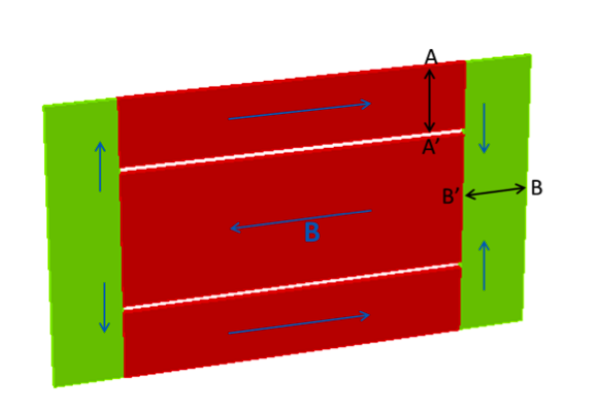
\includegraphics[width=0.45\textwidth]{figures/magnet.png}
%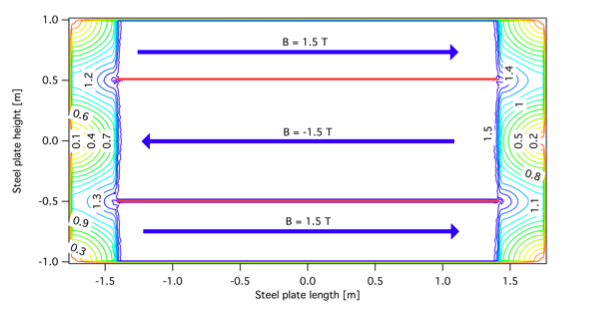
\includegraphics[width=0.45\textwidth]{figures/magnet2.png}
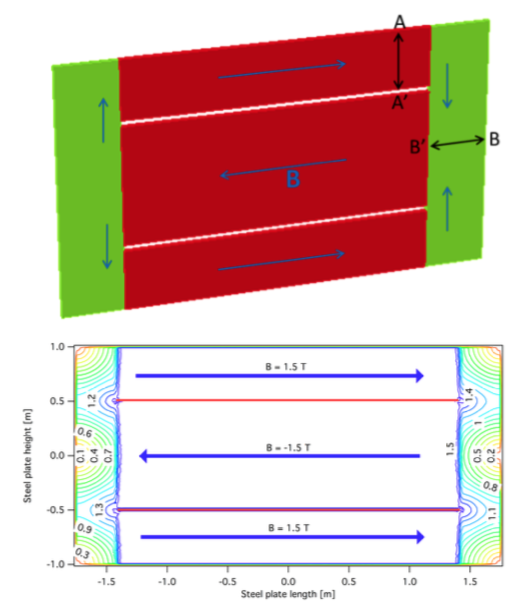
\includegraphics[width=\textwidth]{figures/Mfield.png}
%\caption{(Left) Schematic view of the magnet module. (Right) A contour plot of the magnet module, with the fiducial areas of interest showing magnetic field uniformity.}
\caption{(Top) Schematic view of the magnet module. (Bottom) A contour plot of the magnet module, with the fiducial areas of interest showing magnetic field uniformity.}
\label{fig:mField}
\end{figure}

%\textbf{Field, credit in preface of CERN.}
\subsection{Scintillator modules}
In the Baby MIND, particle hits are detected by scintillating bars which provide both horizontal and vertical position information. There are a total of 18 scintillator modules, where each scintillator module is constructed from 95 horizontal bars for each of the two horizontal planes, $3000 \times 31 \times 7.5$ mm$^3$, and 16 vertical bars, $1950 \times 210 \times 7.5$ mm$^3$ for two planes of vertical bars each providing a total size of the scintillator module as $3000 \times 1950 \times 30$ mm$^3$. Since the vertical information is important for curvature, smaller bars are used to provide a better position resolution. The bars are arranged in 4 planes, of horizontal, vertical, vertical, horizontal, with an overlap between planes to achieve close to 100\% hit efficiency for minimum ionizing muons~\cite{51Saba}. INR Moscow built and designed the scintillator bars, providing a good light yield, figure~\ref{fig:horizontal}~\ref{fig:vertical}, regardless of where the bar is hit. The bars are polystyrene based, 1.5\%PTP, 0.01\% POPOP and held together mechanically within an aluminium support frame  The bars contain Kuraray WLS fibers (200 ppm, S-type, diameter 1.0 mm) and contain a reflective coating 30 to 100 $\mu$m from chemical etching of the surface. The connectors are custom made using Eljen EJ-500 optical cement. A schematic view of the horizontal bars can be seen in \FigRef{fig:horizontal} and the vertical bars in \FigRef{fig:vertical}. 


%Overlap plot?

%The scintillating elements, seen in \FigRef{fig:Vbar}, have been chosen as 18 scintillating modules consisting of four planes per module, two oriented along the horizontal direction with and two oriented in the vertical direction, each to produce good horizontal and vertical resolution of the particle interactions 

\begin{figure}[h!]
\centering
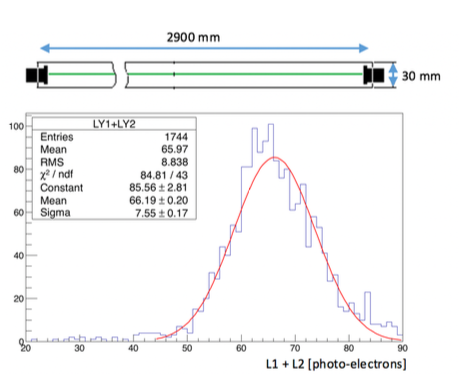
\includegraphics[width=\textwidth]{figures/horizontal.png}
\caption{Schematic view of the horizontal bar and light yield curves.}
\label{fig:horizontal}
\end{figure}


\begin{figure}[h!]
\centering
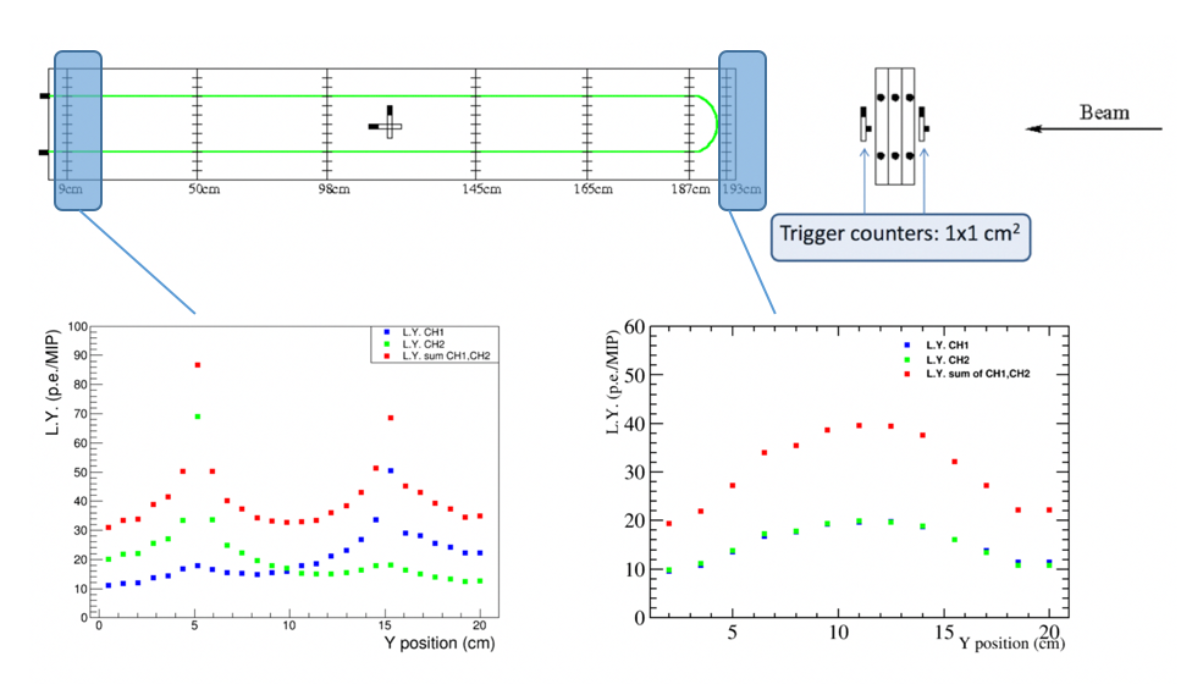
\includegraphics[width=\textwidth]{figures/vertical.png}
\caption{Schematic view of the vertical bar and light yield curves performed for hits at the near and far end of the bar.}
\label{fig:vertical}
\end{figure}


%\begin{figure}[h!]
%\centering
%\includegraphics[width=0.5\textwidth]{figures/Vbar.png}
%\caption{One of the vertical scintillator bars.}
%\label{fig:Vbar}
%\end{figure}

\subsection{Layout}
Design constraints came from the need the need for Baby MIND to operate at both CERN and J-PARC on a relatively short time scale. The installation at J-PARC has driven the overall design with the requirement to lower segments of detector elements through a narrow shaft down to the lowest floor of the ND280 building pit at J-PARC. The magnetisation scheme for the Baby MIND developed within the CERN Neutrino Platform framework is a direct result of this constraint.

Previous magnetised iron detector, discussed in chapter~\ref{c:expIntro}, have been in the kiloton range, Baby MIND is comparatively small weighing only 65 t. A schematic overview of the detector can be seen in \FigRef{fig:design}, showing the full detector composed of 18 scintillator modules, and 33 magnetised ARMCO steel plates, referred to as magnet modules. The full detector is around 4 meters in length with a height of around 2 meters and width of 3.5 meters. The chosen layout of the detector for the test beam is divided into four blocks with first block, block 1, containing 3 sub-blocks and the last block, block 4, containing 2 sub-blocks. The gaps between sub-blocks in block 1 have been added to improve the low momentum reconstruction using a lever-arm approach, discussed further in section~\ref{sec:reconstruction}.

%\textbf{Describe the current J-PARC design as well.}


%As discussed in \SubSectionRef{subsec:MINDdetector}, a MIND type detector requires a magnetized volume as well as interaction medium to deflect the particle tracks and scintillating elements to detect the particle hits. A schematic overview of the detector can be seen in \FigRef{fig:design}. 
\begin{figure}[h!]
\centering
%\includegraphics[width=\textwidth]{figures/design.png}
\includegraphics[width=\textwidth]{figures/MIND.jpeg}
\caption{The test beam Baby MIND design, in yellow the magnet modules and in blue the scintillator modules.}
\label{fig:design}
\end{figure}

%Last layout
%\textbf{iterations, highlight flexibility of design?}

\subsection{Electronics}
The scintillating fibres, present in the bars are read out using Hamamatsu MPPC (Multi Pixel Photon Counters). Compared to PMTs these use a lower voltage, less current and are compatible with magnetic fields. This provides a small size, and simple electronics for the modules. The MPPCs are custom made S12571-025C (and derived S10943-5796), a size of $1\times1$ mm$^2$ (65\% fill factor) and 25 μm cell size. The operating voltage is $\approx 67.5$ V with photon detection efficiency (PDE) ≈ 35\%, gain $5 \times 10^5$ and dark counts of typically 100 kcps. The MPPC signals, sampled at 400 MHz, are powered (HV/LV) and read out by custom made Front End Boards (FEBs), seen in \FigRef{fig:FEB}, designed for 96 channels using CITIROC ASICs~\cite{78EASIROC}. The MPPC signals are connected through a 5 m extension coaxial cable bundle containing up to 32 photosensors signals. The purpose is to decouple the FEBs from the scintillator modules, which improves accessibility to FEBs and their long term maintainability. These rack mounted FEBs have been designed by Geneva University containing $3 \times 32$ channel connectors, 3 CITIROC ASICs with 32 channels each. The FEBs are installed in mini-crates which can connect up to 7 FEBs via readout/slow control on USB3 and/or Gigabit using a backplane seen in~\FigRef{fig:crate}. 
Data is sent from the mini-crates to DAQ computers via USB3 and passed on to a final computer located in a control room. The full readout chain can be seen in the block diagram in \FigRef{fig:daqChain}.

%with a platform independent readout, Windows/Linux. There is also an analog readout, 8 μs for 96-channel low gain and high gain with a 12-bits, 8 channel, 40 MSam- ples/s per channel ADC based on the Altera ARIA5 FPGA. \textbf{Cite Etams paper?}

%with the readout electronics installed in 8 mini-crates on top of the detector. Each mini-crate can accommodate up to 7 Front-End Boards (FEB) (fig. 2). Each FEB can read-out up to 96 detector channels. The data is transferred to the Data Acquisition System (DAQ) via USB 3 interface. The FEBs can work either in standalone mode, in which every FEB is connected to the readout computer via a USB3 connection, or in time division multiplexing (TDM) mode in which all FEBs of a mini-crate are chained and the data is passed to a single USB3 master FEB which sends it to the DAQ. This allows sharing the available data bandwidth and reducing the amount of required cables. There also is a possibility, while in TDM mode, to assign the full USB bandwidth to any selected FEB in the chain.


\begin{figure}[h!]
	\centering
\includegraphics[width=0.48\textwidth]{figures/FEB.png}
\includegraphics[width=0.48\textwidth]{figures/FEB2.png}
\caption{(Left) Schematic view of FEB layout. (Right) An image of the FEB in one of the racks.}
\label{fig:FEB}
\end{figure}

\begin{figure}[h!]
\centering
\includegraphics[width=0.48\textwidth]{figures/crateInstalled.png}
\includegraphics[width=0.48\textwidth]{figures/backplane.png}
\caption{(Left) Front end electronics mini-crate installed on the detector. (Right) Block diagram representing the backplane. Figures from \cite{52Georgi}}
\label{fig:crate}
\end{figure}

\begin{figure}[h!]
\centering
\includegraphics[width=\textwidth]{figures/fullDAQ.png}
\caption{Readout block for the Baby MIND. Figure from \cite{52Georgi}}
\label{fig:daqChain}
\end{figure}



%The Baby MIND electronic readout scheme includes several custom-designed boards [12].  At the heart of the system is the electronics Front End Board (FEB), developed by the University of Geneva, Figure 5. The readout system includes two ancillary boards, the Backplane, and the Master Clock Board (MCB) whose development has been managed by INRNE (Bulgarian Academy of Sciences) collaborators.
%One critical element in the photosensor readout path is the cable bundle, a 5 m extension coaxial cable RG174U that connects the photosensor to the FEB. Each bundle connects up to 32 photosensors. The purpose is to decouple the FEBs from the scintillator modules, which improves accessibility to FEBs and their long term maintainability. The module end of the bundle hosts some electronics that manages the application of the high voltage to the SiPMs, enabling faulty SiPMs to be switched off at that level. This feature was added after the summer 2016 beam tests, where a short circuit on a single channel would disable a bank of 96 channels.

%The FEBv2 hosts 3 CITIROC chips that can each read in signals from 32 SiPMs [13]. Each signal input is processed by a high gain, and a separate low gain, signal path. Both paths comprise independent pre-amplification and "slow" shaping stages with tuneable gain and shaping time con- stant, respectively. The outputs from the slow shapers can be sampled using one of two modes: a mode with an externally applied delay, and a peak detector mode. A faster shaper can be switched to either HG or LG paths, followed by discriminators with adjustable thresholds providing 32 individ- ual trigger outputs and one OR32 trigger output. An Altera ARIA5 FPGA on the FEBv2 samples these trigger outputs at 400 MHz, recording rising and falling times for the individual triggers and assigning time stamps to these. Time-over-threshold from the difference between falling and rising times gives some measure of signal amplitude, used in addition to charge information and useful if there is more than one hit per bar within the deadtime due to the readout of the multiplexed charge output of $\approx$ 9 μs. The ARIA5 also manages the digitization of the sampled CITIROC multiplexed HG and LG outputs via a 12-bit 8-ch ADC.

%The FEBv2 is designed to fit into a slot in a minicrate as shown in Figure 5. The front face receives the SiPMs cable bundles, the rear end plugs into the backplane. Up to 6 FEBv2 can be housed in each minicrate. Eight minicrates are distributed either side of the Baby MIND.
%The internal 400 MHz clock on the FEBv2 can be synchronised to a common 100 MHz clock. The synchronisation subsystem combines input signals from the beam line into a digital synchro- nisation signal (SYNC) and produces a common detector clock (CLK) which can eventually be synchronised to an external experiment clock [14]. Both SYNC and CLK signals are distributed to the FEBs. Tests show the FEB-to-FEB CLK(SYNC) delay difference to be 50 ps (70 ps). Signals from the beam line at WAGASCI include two separate timing signals, arriving 100 ms and 30 μs before the neutrino beam at the near detectors [15]. The spill number is available as a 16-bit signal.

\subsection{Construction and test beam}

The CERN Neutrino Platform approved Baby MIND as experiment NP05 in December 2015 and construction started in August 2016 and finished in June 2017. During the development of the detector it was proposed to use Baby MIND as a muon spectrometer downstream of the WAGASCI experiment (T59) at J-PARC, using neutrinos from the T2K beamline, to provide charge and momentum of outgoing muons from neutrino charged current interactions. The installation and commissioning of the detector in J-PARC will took place in the beginning of 2018, with commissioning in the summer and started to take beam at J-PARC in October 2018.

%\textbf{Discussion what was in the test beam, results in chap 5?}

\newpage
\clearpage

\section{WAGASCI/T59}\label{sec:WAGASCI}

The new WAter-Grid-SCIintilator-detector (WAGASCI) at the J-PARC neutrino beam line will measure the difference in cross sections from neutrinos interacting with a water and scintillator targets, in order to constrain neutrino cross sections in oxygen and carbon, essential for the T2K neutrino oscillation measurements. It follows a similar approach to the one used for iron scintillator cross-sections in the INGRID detector~\cite{21T2K}.

Baby MIND will act as a magnetic spectrometer behind the main WAGASCI target. Baby MIND was installed inside the WAGASCI cavern at J-PARC in the beginning of 2018 to measure the charge and momentum of the outgoing muon from neutrino charged current interactions, to enable full neutrino event reconstruction in WAGASCI.

\subsection{Motivation}
The WAGASCI experiment (T-59) at J-PARC on the T2K beamline aims to improve measurements of the ratio of neutrino interaction cross-sections on water and carbon. This is required to reduce systematics due to nuclear effects in water, currently the dominant systematic uncertainty in the T2K neutrino oscillation analyses~\cite{21T2K} With planned upgrades to the T2K and a planned follow-up project HyperK~\cite{24HyperK}, there is a strong motivation to reduce the systematic uncertainties. The aim is for T2K to improve the level of systematic precision to 4\%. 

%The main goals of the proposed detector are to improve the charge current cross section ratio between water and scintillator targets and to perform high-precision measurement of different charged current neutrino interaction channels.

WAGASCI proposes to test a new 3-D grid-type detector, composed of plastic scintillator and water, to improve on the current understanding of nuclear effects in neutrino interactions. The WAGASCI collaboration states that the detector will be able to measure this cross-section to a level of 3\% systematic uncertainties in the $1 GeV/c$ energy region with a generic MIND~\cite{30WAGASCI}. %\textbf{however no evidence has been given for this claim}. 
Using WAGASCI as a near detector, in the ND280 building, combined with the far Cherenkov detector provides knowledge of the ratio of neutrino interaction cross-sections in water and plastic scintillator. Due to the design of the WAGASCI being both small and not including any magnets, it is impossible to reconstruct charge or momentum for incoming particles. By including the Baby MIND to provide reconstruction downstream, this obstacle is overcome. The size of the Baby MIND is particularly well suited for the WAGASCI experiment providing excellent acceptance for forward secondaries from interactions in the upstream WAGASCI water and carbon targets. During operation with the WAGASCI experiment, Baby MIND is referred to as the Muon Range Detector (MRD). The layout can be seen in \FigRef{fig:WAGASCI}.

%Long baseline neutrino oscillation experiments, amongst others, have confirmed the neutrino sector requires physics beyond the Standard Model. T2K (Tokai-to-Kamioka) discovered electron neutrino appearance in 2013 from a muon neutrino beam with a significance of 7.3σ with a frac- tion of the approved 7.8 × 1020 protons-on-target (POT) [1], using the Super-Kamiokande water Cherenkov located 295 km from the neutrino production site at the J-PARC. Results excluding zero CP violation at 90\% confidence level were announced by T2K in 2016, with data from 20\% of the approved POT. With upgrades to the proton beam, reaching 420 kW in 2016, and projected to reach 800 kW in 2019 and 1.3 MW beyond 2020, there is a strong motivation not to be systematics- limited for future runs at T2K and its follow-up project HyperK \cite{24HyperK}


%The T2K experiment requested an increase in exposure to 20 × 1020 POT, aiming to improve the level of systematic precision to 4\%. The J-PARC T59 experiment [3], referred to as "WAGASCI", will address one of the dominant uncertainties, the knowledge of the ratio of neutrino interaction cross-sections in water (far detector) and plastic scintillator (near detector).
%WAGASCI proposes to test a new 3-D grid-type detector, to improve on the current under- standing of multi-body nuclear effects of neutrino interactions in the 1 GeV energy region, possibly reaching a level of 3\% systematic uncertainties. 

%The 3-D modules have higher target fraction (80\%), and wider angular acceptance (4π) compared with the ND280 near detectors [4]. They are located on the B2 floor of the ND280 building, where different neutrino spectra are available from different off-axis positions. Measurements with different but fractionally overlapping beam spectra will help resolve contributions from different neutrino energies, important for oscillation analyses given the neutrino beam spectrum at a 2.5◦ off-axis angle is not monochromatic.

\begin{figure}[h!]
\centering
\includegraphics[width=\textwidth]{figures/WAGASCI.png}
\caption{The basic structure of the WAGASCI detector including one of the possible designs for the MIND plates. The MIND detector is denoted as Downstream MRD~\cite{30WAGASCI}.}
\label{fig:WAGASCI}
\end{figure}

\subsection{Layout}

%Currently WAGASCI is horizontal or vertical bars with 3D grid submersed in water. Layout is H 3D V 3D H etc etc. \textbf{What is it actually?} 

There are two main elements of the WAGASCI, the central part is a neutrino interaction target which contains water and hydrocarbon, the target is surrounded by muon range detectors (MRDs). The target it self has scintillator bars in different orientation. The current layout is horizontally stacked bars, 3D grid, vertically stacked bars, 3D grid repeated twice providing a total of 8 planes. The 3D grid, seen in~\FigRef{fig:StrucWAGASCI}, is made of thin scintillator bars of $1000\times25\times3$ mm$^3$ put together to form a grid with small pieces cut out to form a full grid, seen in The 3D structure is currently submerged in water to provide the water in which to study neutrino interactions. This design maximizes the fraction of the target material and also provides good particle tracking capabilities allowing to reconstruct tracks emerging at large angles w.r.t. neutrino beam direction. The WAGASCI detector will collect data with both polarities of T2K focusing horn system. The WAGASCI modules are mainly composed of 1280 plastic scintillator bars and a surrounding stainless steel tank. One WAGASCI module consists of 16 scintillator tracking planes, where each plane is an array of 80 scintillator bars fixed within a frame.
The 40 bars, called parallel scintillators, are placed perpendicularly to the beam, and the other 40 bars, called lattice scintillators, are placed in parallel to the beam with hollow cuboid lattice.

WAGASCI has the possibility of being operated both with water-in and water-out providing either a fiducial volume of the module of 188 kg and the mass ratio of scintillator bars to water as 1 : 4 or a fiducial volume of 47 kg and the mass fraction of scintillator bars as 100 \%.

In conjunction with WAGASCI there is also the INGRID proton module and INGRID module. The main MRD, downstream of the target it the Baby MIND. It can all be seen in~\FigRef{fig:WAGASCI} and in \FigRef{fig:StrucWAGASCI}. 

\begin{figure}[h!]
  \centering
  \begin{minipage}[b]{0.59\textwidth}
    \includegraphics[width=\textwidth]{figures/B2Top.jpeg}
    \vspace{2mm}
    \caption{An image showing the B2 environment with (From left) INGRID proton module, WAGASCI, INGRID module and Baby MIND. The side MRDs are in gray.}
    \label{fig:B2environ}
  \end{minipage}
  \hfill
  \begin{minipage}[b]{0.39\textwidth}
    \includegraphics[width=\textwidth]{figures/B2SideUp.jpeg}
       \vspace{2mm}
    \caption{B2 environment seen slightly from the side.}
     \label{fig:B2environ2}
  \end{minipage}
\end{figure}

\begin{figure}[h!]
\centering
\includegraphics[width=\textwidth]{figures/structure2.jpeg}
\caption{The structure of the WAGASCI detector with scintillator bars either horizontally or vertically with a structure to support each the boxes.}
\label{fig:StrucWAGASCI}
\end{figure}

\subsection{Electronics}

Scintillator bars are used as active elements in the WAGASCI detector. The bars are similar to the Baby MIND as they also use WLS fibres to transport light to Hamamatsu MPPCs. The performance of the scintillator bars was measured with a 600 MeV positron beam. The average light yield was found to be 10-18 p.e. and the detection efficiency was better than 99\% for the whole region of scintillator with a threshold set to 1.5 p.e.  The detector performance of the water-in WAGASCI module was checked during the beam operation in 2017.

As front-end electronics of the WAGASCI modules, a Silicon PM Integrated Read-Out Chip (SPIROC) is adopted.
SPIROC is a 36-channel auto-triggered front-end ASIC, and is produced by OMEGA/ IN2P3. 
It not only contains an analog signal processing part such as amplification and shaping of the waveform, but contains a digital signal processing parts such as auto-trigger and timing measurement.
Charge of MPPC signal is sampled by track-and-hold circuit.
A Front-end electronics board, Active Sensor Unit (ASU), has been developed with the SPIROC2D chip, which is the latest version of SPIROC. 
Each readout board is designed to control a 32-channel arrayed MPPC, and 40 of the ASU boards are aligned on the module surface. 
The data acquisition system used for this detector, including back-end boards, has been developed for prototypes of ultra-granular calorimeters for the International Linear Collider (ILC), and independent of the T2K DAQ system.
To synchronize the DAQ system to J- PARC neutrino beam, pre-beam trigger and beam trigger are sent to the clock control card.
The beam trigger signals are converted from optical signals to NIM signals at NIM module on the B2 floor.
In addition, the information of spill number are delivered with 16-bit ECL level signals, and converted to an Ethernet frame by an FPGA evaluation board to be directly sent to the DAQ PC.

\subsection{MRD and Baby MIND}
The WAGASCI detector requires a muon range detector to measure the momentum and charge of outgoing muons to identify the neutrino event and calculate the neutrino cross-section. As mentioned above, Baby MIND provides this role placed after the main target. There are also two much smaller MRDs on either side of the target to measure background muons from other sources or which have been produced from the neutrino beam but will miss the target or Baby MIND. These side MRDs will not be able to provide any momentum or charge information and will only be used as an extra veto plane for acceptance measurements. The layout can be seen in As seen in \FigRef{fig:WAGASCI}. The main event requirements are that the neutrinos decay somewhere in the target and produces a muon within a suitable angle to traverse four scintillator planes of the Baby MIND.

\section{Summary}
In this chapter the Baby MIND and WAGASCI detectors and collaboration has been presented as well as a description of the current status.

\if{0}
\subsection{Sample events}

We successfully observed some neutrino candidate events. Figure \ref{fig:fNU_evt} shows the first event observed by the WAGASCI module. An event display for reconstructed tracks is shown in chapter~\ref{chapter5}.


\subsection{Construction}

\textbf{OLD subsection, relevant?}

WAGASCI, INGRID moduels etc placed in B2 floar when? Build when?

Baby MIND added in March 2018.

Built, unclear when and how.
Unknown, is it built? No information given or public.

Preface, who did what?

%\section{Joining the two detectors}
%Mention event building using the two detectors? Based on spill number given from the beam.

\fi

\if{0}
\section{OLD}
\subsection{Timeline}
The current timeline for the construction of Baby MIND can be seen in \FigRef{fig:timeline}.
These are the following milestones expected to be met by the Baby MIND project:
\begin{itemize}
\item Beam tests characterization at CERN in May 2017.
\item Shipment to Japan in July 2017.
\item Installation in Japan,WAGASCI pit, in September for operation in October 2017.
\end{itemize}

\begin{figure}[h!]
\centering
\includegraphics[width=\textwidth]{figures/timeline.png}
\caption{The current Baby MIND timeline}
\label{fig:timeline}
\end{figure}


\subsection{Collaboration}

\begin{figure}[h!]
\centering
\frame{\includegraphics[width=\textwidth]{figures/Baby_MIND.png}}
\caption{The current Baby MIND collaboration}
\label{fig:collaboration}
\end{figure}

The 3000 Multi-Pixel Photon Counters (MPPC, also known as Silicon Photomultipliers, SiPM) were provided by the University of Glasgow. Glasgow is also responsible for the simulation software.
\subsection{Layout}

%\subsection{Motivation}
%In the white paper? LOI.

\section{WAGASCI/T59}


\subsection{Collaboration}

The current WAGASCI collaboration is given in figure~\ref{fig:collaborationW}.
\begin{figure}[h!]
\centering
\frame{\includegraphics[width=\textwidth]{figures/T59_collaboration_18April2017.pdf}}
\caption{The current WAGASCI collaboration}
\label{fig:collaborationW}
\end{figure}

\subsection{Layout}
A new water-scintillator detector, WAGASCI (WAter- Grid-SCIintilator-Detector) seen in figure~\ref{fig:WAGASCI}, is proposed to reduce the systematic error in the T2K neutrino experiment.

\begin{figure}[h!]
\centering
\includegraphics[width=\textwidth]{figures/WAGASCI.png}
\caption{The basic structure of the WAGASCI detector including one of the possible designs for the MIND plates.~\cite{30WAGASCI}.}
\label{fig:WAGASCI}
\end{figure}

\subsection{Motivation}
The main goals of the proposed detector are to improve the charge current cross section ratio between water and scintillator targets and to perform high-precision measurement of different charged current neutrino interaction channels.

\fi


\chapter{SaRoMaN simulation and software}
%\chapter{Software development}
\label{c:software}

\section{Introduction}

The software environment used for Baby MIND is the Simulation and Reconstruction of Muons and Neutrinos (SaRoMaN) software suite which is a comprehensive software for MIND/nuSTORM detectors and has been developed at the University of Glasgow over several iterations~\cite{27Bross,  53Laing, 54NUFACT2016Hallsjo}. The software has been expanded to be able to model and simulate a generic detector with limitations in the current implementation of the reconstruction. It includes a complete range of functionality for simulating single particle beams through GEANT4~\cite{Geant4}, or neutrino beams, through GENIE~\cite{Genie}, including geometry design, digitisation and reconstruction through RecPack~\cite{RecPack}. The software suite is also shipped with several analysis code examples written in ROOT~\cite{Root}. It has been created exploiting software engineering and object-oriented techniques and implemented in the C++ and Python programming languages. The software is accessible on request from \url{https://lspace.ppe.gla.ac.uk}. 

\section{General structure}
The SaRoMaN software's main design goals have been to promote modularity, provide a single point of entry for the design and input variables and to simplify usage. With this in mind, the SaRoMaN software is split into four main parts which can be replaced or altered independently of the others as long as the input/output flow is conserved. The parts are denoted, wrapper, simulation, digitisation and reconstruction with the main flow regulated by the wrapper seen in \FigRef{fig:codeFlow} and a more detailed view in \FigRef{fig:structure}. Each part will be discussed further below.

\begin{figure}[h!]
\centering
\includegraphics[width=\textwidth]{figures/codeFlow.png}
\caption{Code flow of the SaRoMaN software suite all controlled and handled through a wrapper.}
\label{fig:codeFlow}
\end{figure}

\begin{figure}[h!]
\centering
\includegraphics[width=\textwidth]{figures/Software_structure.pdf}
\caption{Code structure of the SaRoMaN software suite all controlled and handled through a wrapper.}
\label{fig:structure}
\end{figure}

%The second simulation etc etc.
%Add diagram of code, structure etc. Perhaps some code and or file structures in the appendix.
%Plot the overlaying idea and structure. Stress modularity, charge, momentum and particle type

\section{Wrapper}
To simplify the installation, compilation and usage of the other parts in the SaRoMaN suite, a wrapper has been developed in the Python programming language. This wrapper, aside from the above, handles all input variables, file names, writing of configuration files, standardisation of magnetic field maps and geometry, and data flow between the other parts. 

To simplify operation for the user, all of the installation, compilation and running are handled through simple command line inputs with the option of more advanced commands being issued through the use of the Python wrapper class. After installation, SaRoMaN can be run with some default parameters, a full run diagram can be seen in \FigRef{fig:block}.

\begin{figure}[h!]
\centering
\includegraphics[width=\textwidth]{figures/block.pdf}
\caption{Example of how to run a default simulation.}
\label{fig:block}
\end{figure}

\pagebreak
\section{Simulation}
Simulations are used to test and model how particles will interact with a detector model and what scintillator hits can be expected. The outputs from the simulation include the position of the hit on a bar, the location of a bar, the time of the hit and the amount of energy that was deposited. For the studies performed in SaRoMaN, well tested physics models are used in GEANT4; however, the option exists to add new physics and to test new theoretical models.

The simulation comes with two different modes, neutrino or ``single particle''. For neutrino mode, GENIE is first run to generate the neutrino events. The data from these events are run through GEANT4, which includes details of the detector geometry and materials, to create the response of the detector to the particle hits. In the single particle mode, GENIE is not invoked, and one can choose to run with a beam of charged particles of a single species, which are also passed onto GEANT4 that simulates the response of the detector.

%These events are later populated and the detector constructed through GEANT4. In a single particle mode a beam of a single particle type is assumed, GENIE is not called and the simulation and detector construction are handled through GEANT4.

A unique feature is that SaRoMaN uses a single geometry definition for the whole framework, written in the Geometry Description Markup Language (GDML)~\cite{GDML} which is interpreted in GEANT4 and is passed as a simplified .txt file to the reconstruction, which simplifies any changes of the geometry. This GDML file can be used to describe simple detectors, such as a monolithic scintillator module, as well as the full Baby MIND and even any combination of several of these put together in any layout. It is also possible to generate a GDML file from computer-aided design (CAD) software to get all of the constructional details from the detector.

%\pagebreak
\section{Digitisation}
Digitisation is the emulation of the signals expected to be produced by the detector hardware. It needs to handle the response of the electronics and describe the expected output signals, based on input hits in the detector. Any electrical system can be described as providing an output based on the response function of the system and the input signal. The digitisation is based on a description of the response function of the detector for the simulated input.

This is currently done in a simplified way by smearing data with different Poisson or Gaussian distributions to take into account the stochastic nature of the production of the expected signals, as well as handling events which are distinguished by a large time difference. For the Baby MIND detector the algorithms take the horizontal and vertical bar hits and clusters them together to construct $x$, $y$ and $z$ positions along with the energy deposition and time to produce physical hit points. The full program flow can be seen in \FigRef{fig:digi}.

As a way to simplify the integration and implementation, the data acquisition (DAQ) used for the different test beams have been implemented in the digitisation as well. In this mode, real data is given as input and only the clustering takes place. Due to the usage of a single geometry, a token simulation has to be run in this mode as well to properly construct the geometry.

To ensure that all further analysis is performed properly, the output of the digitisation is identical, whether it was simulated or read out through the DAQ.
%there is no way to distinguish data coming out of the digitisation as being simulated or read in through the DAQ.

One of the most difficult design features of Baby MIND is combining hits from both vertical and horizontal bars. It is possible to get hits which cannot be combined without ambiguity. Figure~\ref{fig:BarAmbi} contains an illustration of two sets of simultaneous hits in the vertical and horizontal bars. Think of two separate events, the first one producing the green hits and the second the red hits. Given that the bars only return that they were hit, not the actual position on the bar that was hit it is not possible to distinguish the green hits from the red hits, they would produce the same data. The current method is for the digitisation to create both hits at all times and these hits are then handled by the reconstruction where they can be distinguished by looking at the pattern recognition and the track reconstruction.

\begin{figure}[h!]
\centering
\includegraphics[width=\textwidth]{figures/Digitisation.jpg}
\caption{Program flow for the digitisation.}
\label{fig:digi}
\end{figure}

\begin{figure}[h!]
\centering
\includegraphics[width=0.5\textwidth]{figures/BarsAmbi.jpg}
\caption{Illustration of the difficulty in combining hits in vertical and horizontal bars when there are two or more hits in each bar.}
\label{fig:BarAmbi}
\end{figure}

\subsection{Simulated data}

The digitisation is provided with a .root file~\cite{Root} containing all of the information from the simulation. Given that the data is assumed to be analysed offline, the first task is to separate any hits into event time windows, where hits can be seen as coming from the same particle. The main difficulty is to allow for the particle to fully traverse the detector and to allow a delay in electronics response within the time window. This provides a number of hits in several time bins, denoted as events, without being able to filter the events by using the position information.
%without having any filter by use the position.

After the timing clustering, so-called 3D space points are created by combining the vertical and horizontal bar hits for a specific module. These 3D points are combined to provide an $x$, $y$ and $z$ coordinate. For each bar, coincidence and overlaps are taken into account, as mentioned previously, by creating all of the possible space points allowed by the combination of hits. A clustering algorithm is used to combine the energy, position and hit time of multiple hits, to create one or several clusters each with a discrete position.% based on bar overlap, deposited energy and hit time.

The final step in the digitisation is to smear the value of the deposited energy and hit time based on measured values of propagation time through the scintillator bars, given the simulated hit position and not only the bar position.

\subsection{Data acquisition}
%\textbf{Here or test beam?}

The current data acquisition (DAQ) framework for the Baby MIND detector is based on the event building being carried out offline,  meaning it is processed both after and away from the acquisition to combine the information from multiple FEBs and to create full events offline.

For simplicity, the DAQ converts the acquired data into the same format as expected from a simulation so that the digitisation can be used in the same way. The main difference is that the smearing is only used for simulated data.

%The main difference is that the smearing used for simulated data is turned off. 

In this simplified version of the data acquisition system written for the Baby MIND test beam, the data is stored in different data files specific for each FEB. In the future, the DAQ shall be adapted to merge the data from each FEB, but this was not possible for the test beams. The data from each FEB has channel number, hit time and hit amplitude. The first step is to convert the data into space-positions, using either the vertical or horizontal bar position information and $z-$position. This is carried out by using a database which correlates the FEB and channel number with the knowledge of the physical layout of the detector. The second step is to ensure that each hit position has a corresponding time and amplitude. Step three is to cluster all of the hits in specific time slots, which are equivalent to the event time windows. When this is achieved, several low level filters are performed, to ensure that an event has enough hits to produce at least four 3D space positions in a time slot. After these steps, the data is equivalent to the data produced by a simulation and is processed in the same manner by the reconstruction.%to be passed onto the reconstruction.

%\pagebreak
\section{Reconstruction}\label{sec:reconstruction}
The reconstruction takes the digitised hit data and assembles tracks and vertices. The main physics parameters are the momentum as well as the charge of the particle. The main problems occur when there are overlapping hits with multiple occupancy per bar. In this situation, it is difficult to distinguish between valid hits and to extract the momentum of the track and its charge.
The first problem is handled by removing and adding hits and using a $\chi^2$ analysis through a Kalman fitter package, RecPack~\cite{RecPack}, to find the best trajectory that fits all hits. The second problem is solved through various algorithms to estimate the charge and momentum using different fits.

For simplicity, the reconstruction currently contains a mode denoted as  `` test beam" where it does nothing more than writes out the input data into a final .root file.

\subsection{Structure}
The reconstruction software has been structured to ensure that the software is as modular as possible. It is currently based on the Kalman fitter package known as RecPack~\cite{RecPack} to provide both a framework and back bone for handling track objects. It is still used since it was the first Kalman filter implementation, however, SaRoMaN would benefit from using a bespoke Kalman fitter implementation to ensure its maintenance and reliability, as RecPack is no longer maintained and its documentation is lacking. 
%It is used for historical reasons, however SaRoMaN would benefit from using a Kalman fitter implementation which is still maintained, development, with few and understood bugs and has documentation.

A Kalman fitter is given an underlying model of the trajectory, in our case knowing that particles travel as helices, and a model of the detector as well as other known inputs to the system to form an estimate of the different possible states of the system in a way that is better than using only a single measurement. This is particularly well suited in particle physics where random noise is given through multiple scattering. It can also take into account the energy loss through different materials and keeps track of the varying magnetic field. The measurements can be used in different parts of the detector to estimate both how the particle has and will continue its propagation. Compared to other models, a Kalman fitter has no underlying assumption about the errors being Gaussian.

In high energy physics one frequently faces the problem of modeling the evolution of a dynamic system from a set of experimental measurements. Most reconstruction programs use similar methods. However, in general they are reimplemented for each specific experimental setup. Some examples are fitting algorithms (i.e. Kalman Filter), equations for propagation, random noise estimation (i.e. multiple scattering), model corrections (i.e. energy loss, inhomogeneous magnetic field, and physics measurements.), model conversion, etc. Similarly, the data structure (measurements, tracks, vertices, etc.), which can be generalised as well, depends on the particular implementation. The motivation for using RecPack is due to the combination of these properties into a simple software package.

SaRoMaN has been split into a number of phases: it first initialises the fitter and then it uses an initial pattern classification to choose reconstruction mode. Currently particles and showers are identified, but only muon-like particles are reconstructed. In this identification, a track is produced along with any off-track hits. Finally, the fitter performs a final charge and momentum estimate on the track and tries to fit more tracks to the off-track hits. If this is a neutrino sample, proton/neutron tracks are only built if it finds an initial muon track.

The test beam mode ignores the event classification and uses the fitter to pass information from input through to the final root file.

The reconstruction has been split into several minor tasks.
\begin{itemize}
\item Handling data: Pushing the input data into a final root file.
\item Track building / pattern recognition, given an event, (a time window) can we build a track from this?
\item Fitting, with a candidate track, is it possible to add more hits to the track and make it longer? Is it possible to find secondary tracks? Also, is it possible to estimate the momentum and charge of the track?
\end{itemize}

%How does the code work? When does the split happen? FitTrack in example Event by event. Goes on into fitter. split test beam or normal mode. Test beam only passes on the data with some minor calculations, straight line fit etc. Build planes. Fill planes with hits. After this, into classifier. In classifier, try to build trajectories. Find single "paths/tracks" if not, handle occupancy. Make a plot of this! Have all of the different modes here. Handle low and normal mode. Use or don't use recpack. Chi square analysis, add hits etc etc.  After classifier do a final fitter and write all of the data into a root file. For neutrinos handle short secondary tracks, atleast check for them. In the current implementation all parts use some part of RecPack. Stress modularity. Plot with flow through reconstruction.

\subsection{Pattern recognition}
The pattern recognition tries to estimate if the event is muon-like or not. It starts by looking at the number of hits for a given event. There are currently two main limitations to a track being fitted in SaRoMaN:
\begin{itemize}
\item At least 4 hit modules are required to do any form of charge estimation or track building.
\item At least 10 hit modules are required to perform a Kalman fit.
\end{itemize}
Outside of these limitations, currently only muon track fitting has been implemented. The general assumption is that each event will contain at least one muon track followed by other secondary tracks. If this is not the case the event is discarded. The event filtering is performed very simply by assuming anything that is not a shower is a muon. Single hits here refer to separable space points, meaning that for each $z-$position there is only one unique hit. The aim of the pattern recognition is to find as many tracks with single hits as possible. In the pattern recognition, tracks are built up from so-called track stubs of at least four single hits. As soon as a track stub is created other hits can be added onto the track stub to create a final track using a $\chi^2$ fit as a metric for evaluating which hits to add. This $\chi^2$ analysis is run through the Kalman fitter and requires an initial charge and momentum guess. This means that the best suitable hits are added to the track stub with the remaining hits saved for use in finding secondary tracks. This initial Kalman fitter produces a track with an estimate of the momentum and charge which is further used in the final fitting.

The program flow can be seen as taking in an event consisting of a number of hits and returning a number of tracks along with hits which could not be fitted into any track. Each returned track contains only single hits as well as a momentum and charge estimate. The latter two are then improved by the fitter.

%Given an event, a time selection which can be seen as part of a accelerator spill cycle. Is it possible from the ensemble of hits to find a track or several tracks. Currently makes the assumption that tracks will be separable in space for at least 4 points or that there are 4 planes with single track points as to have an initial track to later add more points into.

\subsection{Fitting}
The fitter's main job is to build tracks and to estimate the momentum and charge of that track. There are two modes, one main mode for events with more than nine hits are passed into the Kalman fitter RecPack. When it is not possible to perform a helical fit and for any track with more than three hits, a self implemented lever-arm approach is used. In both cases RecPack is used to build the tracks, however the momentum and charge reconstruction has to be split depending on the possibility of a helical fit or not. The full helix equation (equations 4.1-4.3 and 4.4-4.6) has a total of nine parameters and takes ten measurements to be fully fitted.  
\begin{align}
x(t) &= a\cos(bt+c)+d\\
y(t) &= e\sin(ft+g) + h\\
z(t) &= kt
\end{align}

The helix can be related to physical quantities as:
%This can also be written in a more helpful way as.
%http://www-jlc.kek.jp/subg/offl/lib/docs/helix_manip/main.html

\begin{align}
x(\phi) &= x_0 + d_p \cos \phi_0 + \frac{\alpha}{\kappa}(\cos \phi_0 - \cos(\phi_0 + \phi))\\ 
y(\phi) &= y_0 + d_p \sin \phi_0 + \frac{\alpha}{\kappa}(\sin \phi_0 - \cos(\phi_0 + \phi))\\
z(\phi) &= z_0 + d_z - \frac{\alpha}{\kappa} \tan \lambda \phi
\end{align}
where $\vec{X} = (x_0, y_0, z_0)$ is the arbitrary helix pivot point, $d_p$ is the distance from the helix to the pivot point in the $xy$ plane, $\phi_0$ is the azimuthal angle from the pivot point with respect to the helix center, $\kappa$ is the signed reciprocal transverse momentum, $d_z$ is the distance of the helix from the pivot point in the z direction, and $\tan\lambda$ is the dip angle. The deflection angle $\phi$ is measured from the pivot point and specifies the position of the charged particle on the helical track. The variable $\kappa$ can be used to relate to the transverse particle momentum, $p_T$ to the magnetic field as 
\begin{align}
 \kappa &=  Q/p_T \\  
 \rho &=  \alpha/\kappa
 \end{align}
where Q is the particle charge, $\rho$ being the signed radius of the helix, and $\alpha \equiv 1/c B$ being a magnetic-field-dependent constant with $c$ as a constant and $B$ the magnetic field strength. The full particle momentum can be obtained as: 
\begin{equation}
\vec{p} = - \frac{Q}{\alpha} \frac{d\vec{X}}{d\phi} = \frac{1}{|\kappa |} 
 \begin{pmatrix}
 -\sin(\phi_0 + \phi)\\
 cos(\phi_0 + \phi)\\
 tan\lambda
 \end{pmatrix}.
\end{equation}

In practice, this fit also takes both energy loss in the detector and multiple scattering into account when calculating the $\chi^2$ values used to fit the parameters. This motivates the requirement for two different modes. If a helical fit is possible RecPack performs the fitting and returns a final fitted helix, within provided measurement errors, with a momentum and charge estimate.

If a helical fit is not possible, denoted as the low momentum case, several different algorithms are used, as discussed in subsection~\ref{ss:lma}.

The fitting is performed using the Kalman filter algorithm, by using this underlying equation and assuming each measurement point has some error. Each measurement point $\vec{X}$ is related to the next through extrapolation of the helical equation and assuming an error: $\vec{X}_{k+1} = \vec{F}_{k+1,k}\vec{X}_k + \vec{w}_k$. It is in this error term where multiple scattering and energy loss is taken into account. The output is then given as: $\vec{Y}_{k} = \vec{H}_{k}\vec{X}_k + \vec{v}_k$. The helical equation goes into forming the matrix $F$ and $H$.

It should be noted that, in Baby MIND, a helix model is an approximation given that there is no fully encompassing magnetic field and various different materials, iron and scintillator, in the detector. A more correct, but much more complex model would be a helix in the iron with straight line segments in between the non-magnetised air gaps and scintillator modules.

\subsection{Low momentum algorithms}\label{ss:lma}
The force applied to a particle travelling through a magnetic field is given by the Lorentz force:
\begin{equation}
\vec{F}=q\frac{\vec{v}\times\vec{B}}{c}
\end{equation}
where $c$ is the speed of light in vacuum, $\vec{v}$ is the velocity, $q$ the charge and $\vec{B}$ the magnetic field vector.

Using Newton's second law one produces the following differential vector equation.
\begin{equation}
\vec{F}=m\vec{a}=m\dot{\vec{v}}=q\frac{\vec{v}\times\vec{B}}{c}
\end{equation}
The solution to this equation is given by:
\begin{equation}
\vec{p}=m\vec{v}=q\frac{\vec{l}\times\vec{B}}{c}
\end{equation} 
where $\vec{p}$ is the momentum of the particle and $\vec{l}=\vec{X}-\vec{X_0}$ is a vector containing the lengths traversed through the magnetic field.

Using the definition of the cross-product, writing this as a scalar equation, using the small angle approximation and writing using S.I. units produces the normally recognisable equation
\begin{equation}
p = 0.3 QB_\bot \frac{|\vec{l}|}{\theta}=0.3 QB_\bot R
\end{equation}
where $p$ is the momentum in MeV/c, the charge $Q$ is in units of $e$, the electron charge, the magnetic field strength $B$ is in Tesla and the radius of curvature $R$ is in m. This is one of the main equations used for momentum reconstruction in SaRoMaN. The charge is then reconstructed using $p/|p|$. 

\begin{figure}[h!]
\centering
\includegraphics[width=0.5\textwidth]{figures/lowP/scattering.jpeg}
\caption{Track bending inside a magnetised iron plate, measured by four scintillator detectors~\cite{117SABA}.}
\label{fig:Scattering}
\end{figure}

A previous study performed in the collaboration showed that the best best way of evaluating the charge using this method comes from comparing both the first and second bending in the detector, seen in~\FigRef{fig:Scattering}, using two different distributions to handle the scattering.

\begin{figure}[h!]
\centering
%\includegraphics[width=0.5\textwidth]{figures/lowP/null.jpg}
\includegraphics[width=0.8\textwidth]{figures/equationFix2.jpg}

\includegraphics[width=0.8\textwidth]{figures/equationFix1.jpg}
\caption{Illustration of the angular distributions and criteria for selecting charge.}
\label{fig:NullHyp}
\end{figure}

Assuming the distribution of multiple scattering angles and the notation in \FigRef{fig:NullHyp}, such as $f(\Delta_1 | \mu )$ representing the distribution of the measured angle $\Delta_1$ given an assumed charge, the choice of charge is given by the ratio of probabilities.

The algorithm returns a $\mu^-$ if 
\begin{equation}
\frac{f_{\mu^-}(\Delta_1)}{f_{\mu^+}(\Delta_1)} > \frac{f_{\mu^+}(\Delta_2)}{f_{\mu^-}(\Delta_2)}
\end{equation}
and it returns a $\mu^+$ if
\begin{equation}
\frac{f_{\mu^+}(\Delta_1)}{f_{\mu^-}(\Delta_1)} > \frac{f_{\mu^-}(\Delta_2)}{f_{\mu^+}(\Delta_2)}
\end{equation}

%link from http://pdg.lbl.gov/2000/passagerpp.pdf
%Also, look at mind_rec/detector.c


The bending angles are calculated from both measurement planes, (or only one if not possible) and tested against a null-hypothesis of having deflection from only multiple scattering~\cite{13PDG} given by:

\begin{equation}
\theta_0 = \frac{13.6 MeV}{\beta cp} z \sqrt{x/X_0}[1+0.038\ln(x/X_0)]
\end{equation}
where $\beta c$ is the velocity, $z$ is the number of elemetary charges of the incident particle and $x/X_0$ is the thickness of the scattering medium in radiation lengths.

The probability, using this notation, is given in equation~\ref{eq:probScatt}:
\begin{equation}
P_{\mu^\pm} = \frac{1}{2\pi} e^{-(\theta\pm\Delta)^2 / 2\theta_0^2}
\label{eq:probScatt}
\end{equation}

Another goal of the reconstruction is to estimate the momentum. Many different methods using the scattering width or fits have been studied to reconstruct this value in a low momentum region, however the current best approach is to use the continuous slowing down approximation (CSDA). CSDA is based on knowledge of the energy loss in the material before a certain measurement in the detector, assuming the particle deposits an average energy in all materials which it passes. The modular nature of Baby MIND and the varying distance between iron and scintillator planes implies that it has a non-uniform material description. The range of a particle in the detector can be used to extract an initial estimate of the momentum of the particle, and the uncertainty associated with this estimate depends on the number of iron plates between specific scintillator modules. For example, if there are three iron modules between scintillators the error on the momentum is estimated to be approximately $\sqrt{2} \times 90 MeV/c$. Combining information from the CSDA and the angle produces the final momentum and charge estimate.

%This method cannot be used for tracks which pass through the full detector as then the error is impossible to estimate. 

%If the angular estimate does not work due to multiple scattering a final estimate is used by using a quadratic fit for the few hits provided.

At low momentum, when tracks do not penetrate into Baby MIND very much, a quadratic fit for the first four hits can be carried out to estimate the momentum.

\if{0}
Use the angles to and probability to calculate the charge. Momentum currently from range. Seems better.
Probability of angle from multiple scattering, or from magnetic field. 
Momentum comes from the range calculation, see detector layout. Major gaps in monument,  Potentially could and perhaps should use range momentum as long as tracks stop in detector. Problem with steps, helix better.
We have steps in the tracking detectors.
This seems to be the best approach. If this for some reason fails it goes on to a final attempt.
Quadratic fit, given few hits, try to fit to return charge. Use this only for charge. Momentum from range momentum.
\fi

\subsection{Performance}

%\textbf{Add event display! also for testbeam in next chapter}

During development of SaRoMaN two main metrics were used to evaluate performance, track reconstruction efficiency and charge reconstruction efficiency. These metrics are evaluated by determining how many simulated tracks can be reconstructed compared to the total number of simulated tracks and how many of those reconstructed tracks have the correct charge. This is done for muons of both charges and different momentum values.

Performance will be shown for the initially proposed layout of Baby MIND, for which the software algorithms were designed, the layout implemented for the CERN test beam, and a final study based on the layout used for the WAGASCI detector. The main difference between the initial and test beam layout was to remove the initial measurement plane d0, restructuring a few of the blocks and adding gaps between each of the blocks, as seen in \FigRef{fig:oldMIND}. %This was done from a constructional not a physics motivation.

The charge identification is however improved when utilizing a measurement point from a neutrino target, the WAGASCI module upstream of Baby MIND; however, this will reduce the lower energy limit of reconstruction since the muons must traverse the material of the WAGASCI. 

\begin{figure}[h!]
\centering
\includegraphics[width=0.75\textwidth]{figures/oldStudies/oldMIND.png}

\includegraphics[width=0.75\textwidth]{figures/MIND.jpeg}
%\includegraphics[width=0.48\textwidth]{figures/oldStudies/MINDetam.jpeg}
\caption{(Top) Image of the initial Baby MIND layout. (Bottom) The current Baby MIND layout. The main differences consist of removing the first scintillator plane, a different configuration layout in the middle blocks and removing the final scintillator plane. This was done for constructional reasons to be able to transport the detector from CERN to J-PARC.}
\label{fig:oldMIND}
\end{figure}

In \FigRef{fig:oldMIND2} results for the initially proposed geometry can be seen. The plots have been generated by simulating negative and positive muons in the SaRoMaN framework. The results for the slightly changed test beam geometry layout can be seen in  \FigRef{fig:TestBeamMIND2}. 

The main difference between the results are both below 1~$GeV/c$ and in the region above 1~$GeV/c$ and below 2~$GeV/c$. Below 1~$GeV/c$ the charge reconstruction is slightly worse for the test beam geometry, which can be attributed to the removal of the first scintillating plate d0. There is also a slight change in the shape of the reconstruction efficiency above 1~$GeV/c$ and below 2~$GeV/c$, related to the change of the structure of the detector and additions of gaps providing some drift between measurement positions. For both of the layouts the reconstruction efficiency $> 95\%$ above 0.7~$GeV/c$ and its charge identification efficiency is $> 95\%$ above 0.7~$GeV/c$. For the full region both reconstruction and charge identification efficiencies are $> 80\% $. 

\begin{figure}[h!]
\centering
\includegraphics[width=0.8\textwidth]{figures/oldStudies/oldRecEff.png}

\includegraphics[width=0.8\textwidth]{figures/oldStudies/oldChargeID.png}
\caption{Reconstruction efficiency and charge identification efficiency of the initial Baby MIND layout using the SaRoMaN simulation and reconstruction package. The low momentum points in the top figure are based on a different algorithm and definition as they do not require the identification of tracks. Also note that in both figures the points sit on top of each other with red covering blue.}
\label{fig:oldMIND2}
\end{figure}

\begin{figure}[h!]
\centering
\includegraphics[width=0.8\textwidth]{figures/oldStudies/FullFitted.pdf}

\includegraphics[width=0.8\textwidth]{figures/oldStudies/FullChargeID.pdf}
\caption{Reconstruction efficiency and charge identification efficiency of simulated events for the Baby MIND layout configured for the CERN test beam, using the SaRoMaN simulation and reconstruction package. The dip in the top figure represents the boundary as tracks leave the detector where the algorithm.}
\label{fig:TestBeamMIND2}
\end{figure}

%\textbf{Perhaps momentum rec plots as well? Look at old material/collaboration meeting 2 with pull and residuals.}
%\textbf{One plot comparing all of these? Can we compare them? Lower momentum due to TASD?}
\if{0}
Give for different layouts. The initial, well worked. Then work down to the test beam layout and perhaps the latest J-parc layout? 
Charge id, fitting id, momentum pulls and so on.
Look at muons/pions. pure beams with and without TASD/WAGASCI. Especially test beam layout and J-Parc.
Add in the new layout studies?
Quite good, add that charge ID is about x for range y and so on.  Could be improved by changing layout, perhaps even tweaking algorithms etc etc but want to keep generic algorithms to handle different designs.
Momentum pulls and comparisons? Large RMS from RecPack and difficult geometry. Room for improvement.
\textbf{Perhaps cite my Uppsala proceedings?} ~\cite{82Uppsala}.
\fi

\subsection{Unpacking of data}

%\textbf{Based on the FEB readoutprotocol v2.6.}

Currently data has to be recorded by the front-end board and handled by a test beam computer system. The full data contained in the spills has to be written to disk and then it can be processed off-line after the data taking.

The format consists of a time slot, with a time-division multiplexing index (TDM), containing a spill with several triggers. Each global trigger (GTRIG) contains all of the hit data from the various channels at all the times inside the trigger. Hit data contains amplitude and time measurements with the channel information.
Each time measurement comes in steps of 2.5 ns so the system can only distinguish hits on a channel if they happen more than 2.5 ns apart. The triggers come in blocks of 10 $\mu$s resulting in at most 4000 events per channel per trigger. The format can be seen in \FigRef{fig:FEBstructure}.


\begin{figure}[h!]
\centering
\includegraphics[width=\textwidth]{figures/febstructure.jpeg}
\caption{TDM, GTRIG, spill and data structure for the FEB readout communication. Figure, courtesy of Yannick Favre}
\label{fig:FEBstructure}
\end{figure}

%Add data plots perhaps? Not sure what goes here.
%Should I add details about the data format?
%Explain how the unpacking works, the main data structure assumed in the electronics. The main problem with the data structure, how it is not aimed to work online. 
%Read and use documentation from Yordan Ivanov Karadzhov. Also look at what Aleksander/Sascha has done and what is in the code.


\subsection{Particle identification}
Machine learning algorithms are used through the Toolkit for Multivariate Data Analysis with ROOT (TMVA)~\cite{TMVA} for particle identification. The main goal of the particle identification is to identify muon tracks from other background events with high efficiency. There are several filters trying to perform particle identification; however, TMVA is needed to further improve this identification. This will be described in chapter~\ref{c:Testbeam}.

%\subsection{Analysis software}
%Start by combining, if needed, several root files. Continue by choosing interesting root branches, with or without filtering/cutting the data.
%add analysis flows. What is a normal data flow? Add parts to appendix, more data etc etc etc.

%Final root file, read in trees, filter out bad events, if any. Compare apples to apples. 

%\pagebreak
\section{Future development}
Based on the main principles of easily shareable code, using the latest versions and simplicity, a further development of SaRoMaN has already commenced by creating a fully new version based on newer versions of the third party software packages such as GEANT4, GENIE and ROOT. By moving to the latest versions and ensuring that they will be easy to maintain the software becomes ``future proof'' which is very important for ensuring that the results are making use of the latest physics software. The new framework, following the Lord of the Rings theme~\cite{79tolkien2012lord}, has been named SAURON (Simulation And Universal Reconstruction Of Neutrino-like events). SAURON also makes sure to only use open source software and has thus moved from the RecPack Kalman filter to use a Runge-Kutta and Kalman open source fitter known as GENFIT~\cite{81Genfit}. The change of fitter significantly improved the track reconstruction and momentum reconstruction.
The software environment and code can be found in a docker environment at: \url{https://hub.docker.com/r/patha325/science/}. The code is hosted at : \url{https://github.com/patha325/NewSaRoMaN}.

The simulation is based on a generic GEANT4 simulation, which takes in neutrino data simulated with the GENIE open source code used by many. The reconstruction package  GENFIT~\cite{81Genfit}, used by several different experiments, takes generic points and uses a Runge-Kutta method to fit the points and calculate the track momentum and charge.

In a similar way to SaRoMaN, the running is handled by a very simple python script which ensures that all software runs coherently with each other. The geometry is handled in a GDML file and read through all different parts to provide one single point of entry for the geometry. To ensure that the code can be used by anyone on different machines without a difficult installation process, the full software is provided in a docker container which means that the code can be run on any operating system. 

To be compatible with the DAQ unpacking software developed for Baby MIND, a secondary docker container has been created to handle the specific root version requirement as well as some other minor software requirements which all clash with the SAURON container.

SAURON is currently in a state were it can be seen as a simplified and novel version of SaRoMaN. Bar representation, clustering and pattern recognition is not currently implemented in the reconstruction, these are all handled by using truth information from the simulation or provided as extra information. None of these are seen to have a major impact on the results, but should be implemented in a future version. In a similar way, the DAQ unpacking is not included, instead the data is assumed to have been processed through it before being passed into the reconstruction. There are currently discussions regarding a unification of the DAQ unpacking and SAURON.

\subsection{Containers}
One of the main issues with scientific software is that they are developed by small teams, often not made publicly available and often the knowledge is only spread through scientific papers. This means that there are many great software solutions and packages which are not used by scientific collaborations, or are misused due to a lack of communication. One could argue that code should be easy to read and that the purpose of a piece of software should be easy to understand, however this assumes that all developers follow some form of coding standard and has/takes the time to develop their code properly which is often not the case. The clear solution to this problem would be to spend more time documenting and cleaning up code as well as sharing it publicly. One problem which may arise is the use of specific third party software versions which make installation quite difficult especially in a climate where documentation is not prioritised and where software is constantly in development.

One proposed solution which solves the problem would be to provide a full runnable coding platform such as a virtual machine. The benefits are numerous, however most of these are further improved by moving to a new software technique known as a container.

\subsubsection{Container vs Virtual machine}

A container is similar to a Virtual machine (VM) but without requiring any abstraction of hardware, they also run on the OS kernel not requiring an added layer. In essence, a container includes an application with the code and all its dependencies without also requiring a full copy of an operating system. This reduces the size of a container compared to a VM and decreases boot time.
%n handle more applications and require fewer VMs and Operating systems.

\subsubsection{Container for particle physics simulations}
There exist several containers which can be combined for various particle physics simulations. There is currently an official version of the root software in a container \url{https://root.cern.ch/root-docker-container-alpha-version} as well as various unofficial containers for software such as GEANT4.

During the development of SAURON, early versions of the container provide good tools for running particle physics simulations, without providing the SAURON framework or the neutrino specific parts. There are also early versions which provide the GENIE neutrino generator which provides a good starting point for running neutrino simulations.

\if{0}
\subsection{Machine learning in particle physics}

There has been some development of using machine learning techniques for various physics analysis as well as in event selection or particle identification for events in detectors. Focusing on the neutrino physics field, there have been a lot of interesting articles relating to how to identify neutrino events in Argon detectors using machine learning~\cite{83Radovic2018, 84Adams}. 

%In the field of neutrino physics machine learning is not often used, some plots for dune etc etc. This was used in this collaboration using TMVA for particle identification/particle selections to chose muons in a background sample for the test beam.
%For the reconstruction, kalman filtering and cellular automaton for few hit events, are used as well.
%Outside of this novel software frameworks such as virtual machines, docker containers and continuous integration techniques have been used.

%What is machine learning? How is it used today? Techniques for particle physics etc. novel ML techniques.

%\subsubsection{Machine learning in particle physics}

%\subsubsection{Machine learning applied to event identification}

%Show TMVA plots, comparing normal likelihood techniques to machine learning, different applications and different methods. Explain the different methods.

%Relating more to data science than expected results from physics.

%Already been done, needs improvement.

\subsection{Other good practises}

\subsubsection{Versioning}
Currently the software is provided as is without any main release or naming convention. It would be beneficial to adapt a good versioning convention by tagging the software on gitlab. The container used has been provided with version numbers in an adhoc manor which should be tied into the software version number.

\subsubsection{Continuous integration}
For the SaRoMaN software a continuous integration platform was provided to ensure that installation of third party software as well as simple test analysis would always work regardless of bad committed code or broken download links. Something similar has been started for SAURON but not implemented fully and it is clear that it could be extended with thorough analysis and more specific test examples.

\subsubsection{Documenting}
Due to the time constraint no documentation exists for either of the software frameworks. The direct recommendation would be to spend time developing some doxygen documentation for the SAURON framework along with an easy how-to guide for new users.
\fi
\section{Summary}
In this chapter the software framework for Baby MIND has been described, as well as future ongoing developments for improving the software framework. The reconstruction and charge identification efficiencies were evaluated for a series of Baby MIND detector configurations, using the SaRoMaN simulation and reconstruction software, showing that it can deliver high efficiencies over a large momentum range from sub-GeV/c to 10 GeV/c muon momenta.
%There has been a short discussion detailing the some of the metrics used for evaluation and discussion on how to continue the software development.


\input{"5-Testbeam/testbeam.tex"}

\chapter{Neutrino interaction studies}
\label{c:neutrino}

The Baby MIND is build to reconstruct muon tracks passing through the detector. This makes it ideal to be used for muon neutrino reconstruction with an appropriate target. As discussed in subsection~\ref{subsection:Neutrino interactions} there are only a few interactions which produce a free muon which can then be reconstructed with the Baby MIND. These are the muon neutrino charge current interactions, quasi-elastic charge current interactions, deep inelastic scattering and resonant interactions each at various energy ranges as can be seen in \FigRef{fig:neutrinoInteractionsFig}

\begin{figure}[h!]
\centering
\includegraphics[width=0.9\textwidth]{figures/figs_zeller-total-numode.png}
\caption{Neutrino cross sections, showing the quasi-elastic, deep inelastic and single pion cross sections in the GeV range. Taken from~\cite{82McFarland} modified from original made by G.P.~Zeller~\cite{13PDG} containing data points from various experiments.}
\label{fig:neutrinoInteractionsFig}
\end{figure}

The signature for each of these interactions are quite different as a charge-current quasi-elastic interaction will produce a clean proton and muon track, compared to a shower like pion track or the less clear DIS signature. Baby MIND is designed to operate at a lower energy spectrum, below 5 GeV, meaning that the contribution will be mostly from CCQE and pion interactions. Results from various simulations with the T2K near detector beam spectrum and data recorded from the commissioning will be showed.

%Lab report again, trying to estimate cross-section of interactions. Why? Need it to improve oscillation measurements. Using simulations of muon neutrinos from simulation. What is done, what cuts? How Do we calculate cross-sections? Angular acceptance, look at what Marc has done, do similar things and further the calculations.Discuss what to expect, what kind of interactions could happen in the TASD/WAGASCI? What could be seen? What information? Baby MIND can also have interactions, which ones would be visible? Can reconstruct muons in Baby MIND, electrons and pions visible and potentially reconstructable, but not now. Charge id, momentum. Identifying muons comming of the neutrino interaction with a specific beam and interaction area. Describe the fiducial volume like in my talk for NuFACT.

\section{Muon charge current quasi-elastic}

CCQE interactions produce a clear muon track for both neutrinos and anti-neutrinos, however the interaction only produces a proton track for neutrino interactions as seen below:
\begin{align}
\nu_\mu + n &\rightarrow \mu^- + p\\
 \bar{\nu_\mu} + p &\rightarrow \mu^+ + n
\end{align}

For the neutrino interactions, this becomes a very clear signature in a fully active target where both a muon and proton track can be identified. For anti-neutrinos this is not possible since neutron tracks are usually not detectable for most detector types. However the main goal is to identify muon tracks from pion tracks which is simply identifying a shower from a track. There have been a lot of interesting articles relating to how to identify neutrino events in Argon detectors using machine learning~\cite{83Radovic2018}~\cite{84Adams}. In a non active target it becomes very difficult to identify neutrino interactions as pions may decay to muons and become indistinguishable from directly produced muons.

%Direct simulations with CCQE and different geometries. Use data from specifically Baby MIND in B2 beam line. Explain the beam line etc etc.

%CCQE from muon neutrino produces a muon. Clear production and easy to identify in TASD, not possible in MIND due to the design. 

%Acceptance study, detector layout. Beam settings? Add charge reconstruction, momentum reconstruction. Particle ID? also need interaction ID from TMVA.

%Different size gap, different detector layout both early/testbeam and new at Japan. Cross-section studies. Look at what Marc has done!  Discuss with paul what and how to do cross-section measurements.

\pagebreak
\subsection{Interactions in TASD + Baby MIND}

During the construction of Baby MIND, it was proposed to potentially fully instrument the whole TASD, used during the first beam test, and use it as a fully active target to be combined with Baby MIND, illustrated in~\FigRef{fig:TASDandMIND}.

\begin{figure}[h!]
\centering
\includegraphics[width=0.9\textwidth]{figures/MINDAida.jpeg}
\caption{An illustrative sketch of the detector setup with the TASD detector in front of Baby MIND.}
\label{fig:TASDandMIND}
\end{figure}

For all analysis the TASD is used as a CCQE identification and neutrino veto, expecting two tracks (neutrino) or atleast start of muon track. The dimentions are the same as mentioned under the test beam section, with a distance of 368mm between the two detectors. Neutrinos are simulated using the T2K near detector spectrum in reverse horn current mode (RHC), seen in~\FigRef{fig:T2KndSpectrum} in the SAURON framework. 



In the framework several figures of merit are produced, the muon energy spectrum, reconstructed muon energy spectrum, reconstructability of tracks vs energy and charge reconstruction vs energy. All of these figures of merit are shown in~\FigRef{fig:T2KTASDfitted} and~\FigRef{fig:T2KTASDfittedcharge}.

\begin{figure}[h!]
\centering
\includegraphics[width=0.9\textwidth]{figures/WAGASCIflux.jpeg}
\caption{The energy spectrum for muon neutrinos and muon anti-neutrinos in the T2K near detector RHC beam.}
\label{fig:T2KndSpectrum}
\end{figure}

\begin{figure}[h!]
\centering
\includegraphics[width=.9\textwidth]{figures/NeutrinoChap/data260618/T2K/FittedT2KNeutrinoBeamMIND.pdf}
\caption{The efficiency plot of how well the algorithm can reconstruct neutrino tracks vs muon momenta for simulated tracks interacting in the TASD.}
\label{fig:T2KTASDfitted}
\end{figure}

\begin{figure}[h!]
\centering
\includegraphics[width=.9\textwidth]{figures/NeutrinoChap/data260618/T2K/ChargeIDT2KNeutrinoBeamMIND.pdf}
\caption{The efficiency plot of how well the algorithm can reconstruct muon charge vs muon momenta for tracks fitted in the algorithm.}
\label{fig:T2KTASDfittedcharge}
\end{figure}





Similarly to the simulated muon beam, and data the charge reconstruction efficiency is very good for the reconstructable tracks. The difference comes from the fact that the neutrinos are produced at angles instead of straight on the center of the detector (with some beam size).Muons from neutrinos are produced at all angles depending on the kinematics of the neutrino interaction and neutrino energy. 


Reshow the muon beam? Discussion about angle etc...



Have simulations both for T2K and NuSTORM beamline, describe both.
Full analysis in MIND, only TASD as veto.
 Shown at NuSTORM talk, fix momentum slightly.
 
\pagebreak
\subsection{Neutrino interactions in Iron in Baby MIND}
Simulations for a  T2K like beam, explain the details and event selection, (None for simulation but easy enough with data). Use the specific fiducial volume. Set up at J-PARC, all the details with that.

To compare simulations with data taken for the commissioning run interactions had to be simulated in the IRON of the Baby MIND due to the fact that the WAGASCI data taking can as of yet not be joined with the Baby MIND data.

\begin{figure}[h!]
\centering
\includegraphics[width=.9\textwidth]{figures/NeutrinoChap/Neutrino/T2KIronRecEff.pdf}
\caption{The efficiency plot of how well the algorithm can reconstruct neutrino tracks vs muon momenta for simulated tracks interacting in the Iron.}
\label{fig:IronMINDfitted}
\end{figure}

\begin{figure}[h!]
\centering
\includegraphics[width=.9\textwidth]{figures/NeutrinoChap/Neutrino/T2KIronChargeEff.pdf}
\caption{The efficiency plot of how well the algorithm can reconstruct muon charge vs muon momenta for tracks fitted in the algorithm.}
\label{fig:IronMINDfittedcharge}
\end{figure}

\pagebreak
\subsubsection{Simulations vs data}
Show same as for nuFact, explain in detail what was done. Show the data.

\pagebreak
\section{Future studies}

\subsection{Neutrino interactions in WAGASCI + Baby MIND}

Using WAGASCI as a CCQE identification,

\subsubsection{Interactions in the full WAGASCI}

Discuss future data taking, interactions everywhere etc etc.

%\subsection{GAr + BabyMIND}
%\subsubsection{Analysis Simulations}
%\subsection{TASD + BabyMIND}
%\subsubsection{Analysis Simulations}
%\subsection{Full WAGASCI}
%\subsubsection{Analysis with Simulations}
%\subsubsection{Simulations vs data}

%\section{Electron charge current quasi-elastic}



\input{"7-NSI/NSI.tex"}

\chapter{Conclusions and Outlook}
\label{c:conclusion}

\section{Baby MIND}

\section{Software}



%\input{"2-main/babyMINDintro.tex"}

%\input{"2-main/babyMINDdata.tex"}

%\input{"2-main/Phenom.tex"}


% -----------------------------------------------------------------------------
\appendix

\chapter{An Appendix}
\label{a:appendix}

This is an appendix.


% -----------------------------------------------------------------------------
\newpage

\input{"footer.tex"}

